\newpage
\section{DBM experiments}
\subsection{Experiments on MNIST}
\subsubsection{Before sparsity targets, AIS}
Architecture and hyperparameters initially were similar to those of \cite{dbm_code}, however, I observe that learning rate should be smaller (eventually I used exactly 1 order of magnitude smaller starting learning rate).
\clearpage

\begin{figure}[h]
\begin{mdframed}
\centering
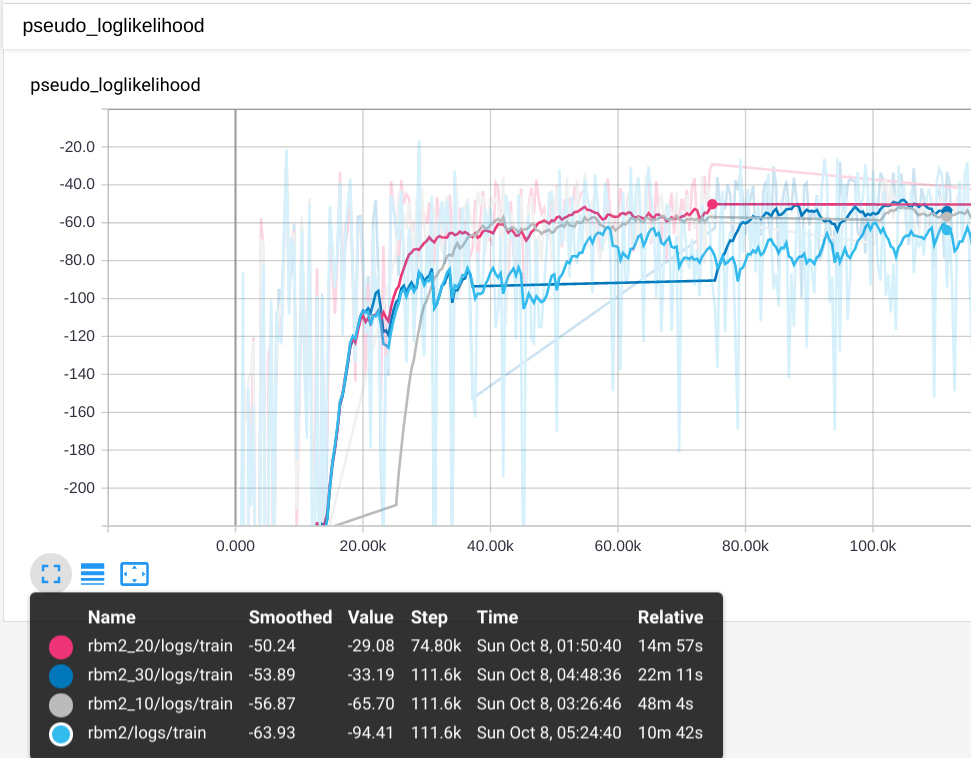
\includegraphics[width=4.2in]{dbm-mnist/rbm2_pll.png}
\\[1em]
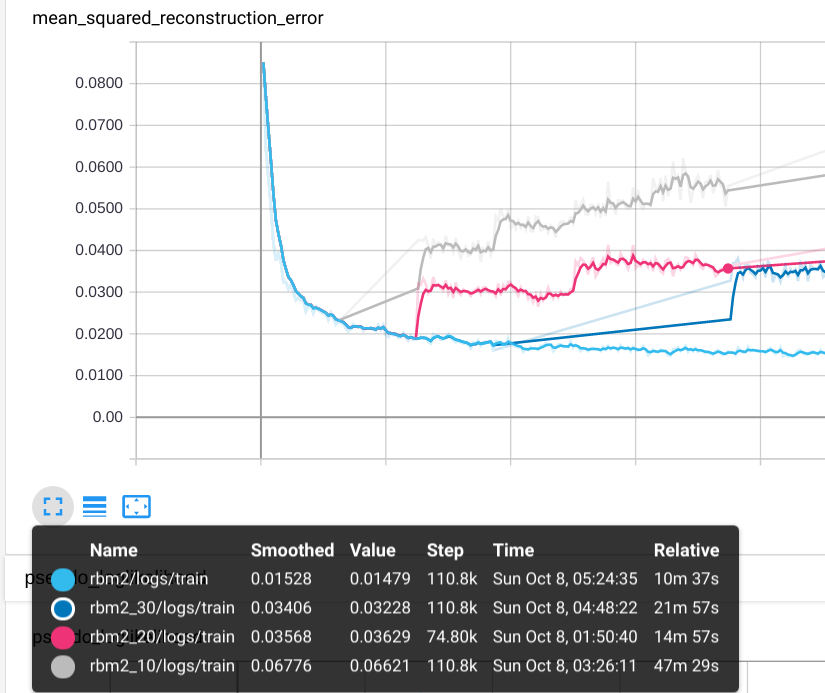
\includegraphics[width=4.2in]{dbm-mnist/rbm2_msre.png}
\caption{PLL and reconstruction error for RBM \#2 trained on extracted features $\mb{q}_i=p(\mb{h}|\mb{v}=\mb{x}_i; \bs{\psi})$ using RBM \#1 trained on MNIST. $\texttt{rbm\_n}$ means every $n$ epochs number of Gibbs sampling increased by 1, and learning rate $\alpha_t\leftarrow \frac{\alpha_0}{n}$. This approach \cite{dbm_code, salakhutdinov2007restricted} has quite noticeably higher PLL compared to CD-k with constant $k$ (both 1 or higher).}
\end{mdframed}
\end{figure}

\clearpage

\begin{figure}[h]
\begin{mdframed}
\centering
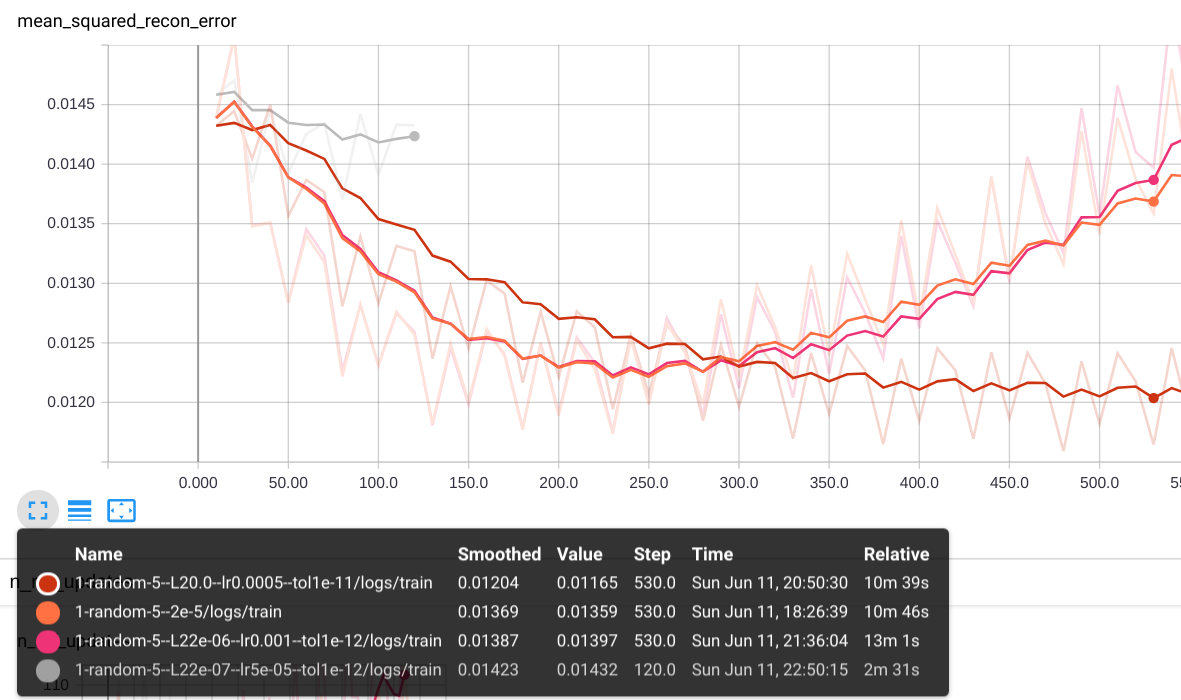
\includegraphics[width=6in]{dbm-mnist/L2_5k.png}
\caption{This illustrates how the use of L2 weight decay harms joint training of DBM in terms of MSRE (no matter how small $\lambda$ is). \u{The intuition} here is when weights are not trained well enough for them to be useful for modeling the data, the weight decay term will drive them to become very small, and they will never have an opportunity to recover. In \cite{goodfellow2013joint} and \cite{goodfellow2013multi} the authors had the same issue and suggested to use \emph{maxnorm} regularization instead. Trained on random subset of 5k images.}
\end{mdframed}
\end{figure}

\clearpage

\begin{figure}[h]
\begin{mdframed}
\centering
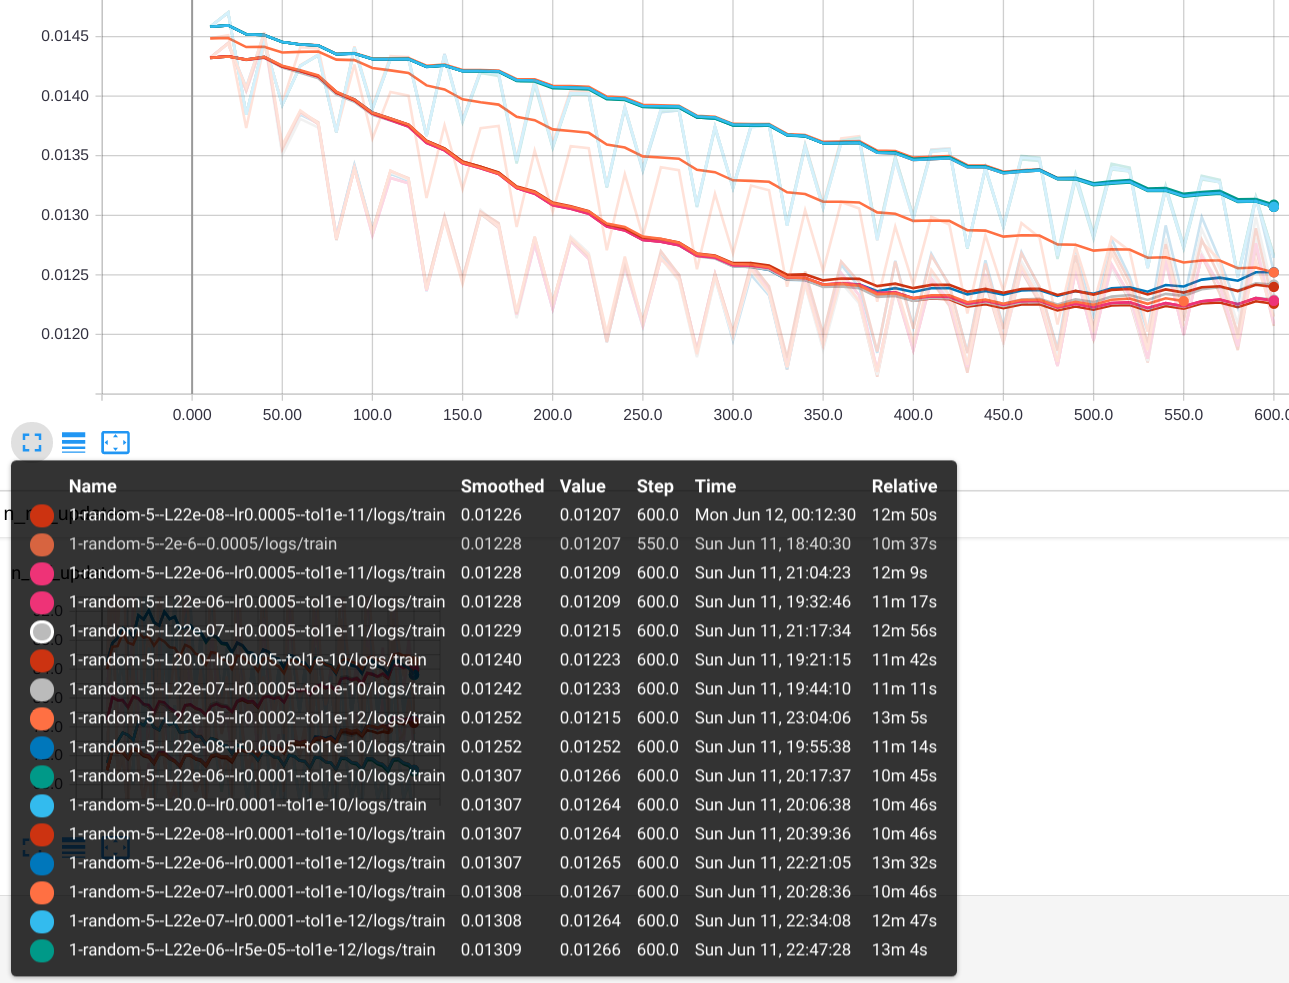
\includegraphics[width=4.6in]{dbm-mnist/L2_lr_tol_5k.png}
\\[2em]
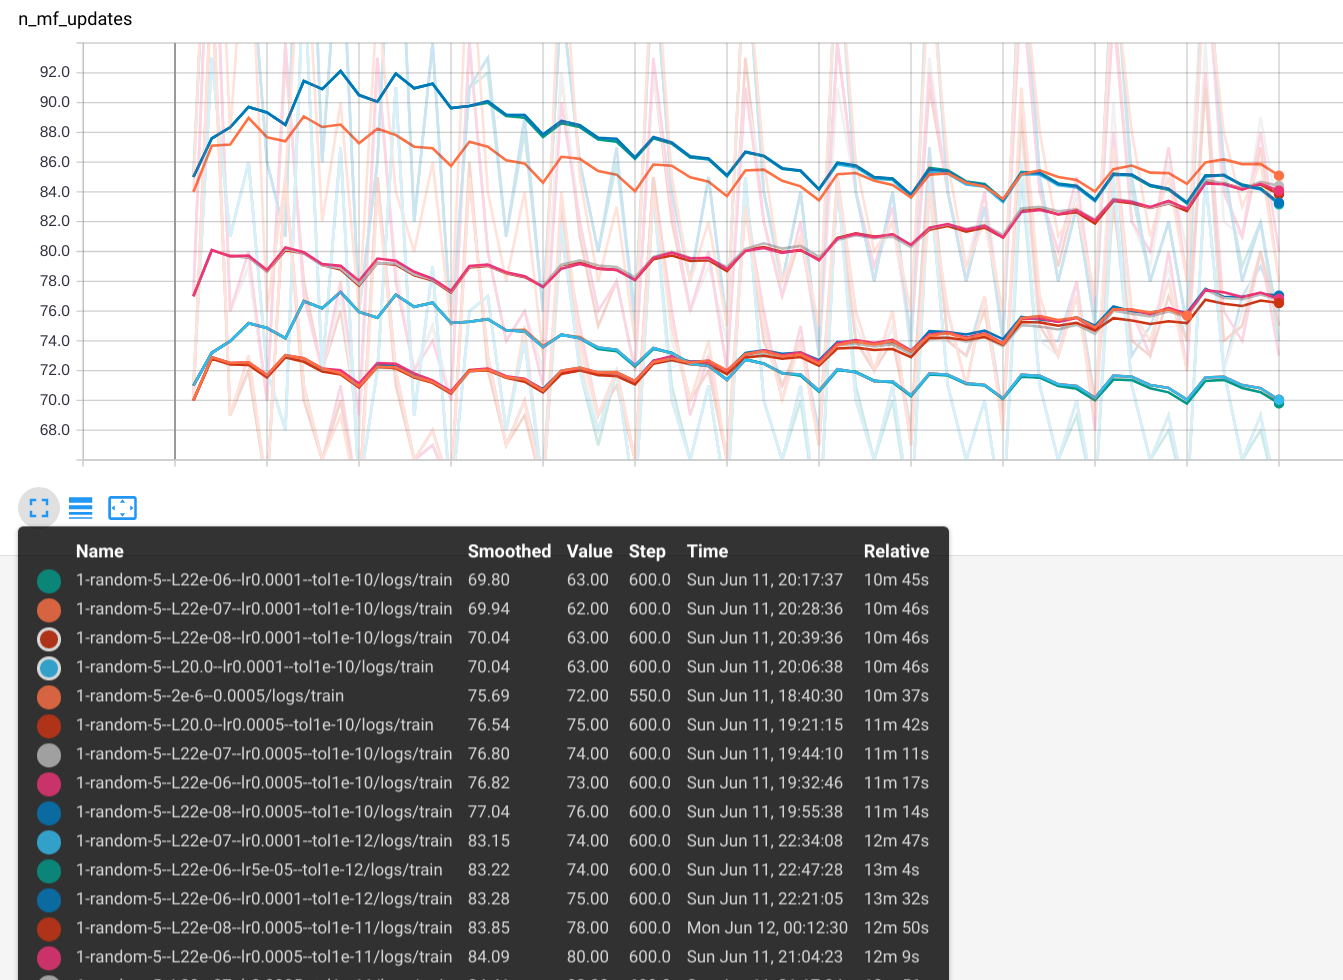
\includegraphics[width=4.6in]{dbm-mnist/n_mf_upd_5k.png}
\caption{The effect of various choices of L2 weight decay coefficient, learning rate and desired mean field tolerance in terms of reconstruction error and number of mean-filed updates to achieve desired tolerance on random subset of 5k images.}
\end{mdframed}
\end{figure}

\clearpage

\begin{figure}[h]
\begin{mdframed}
\centering
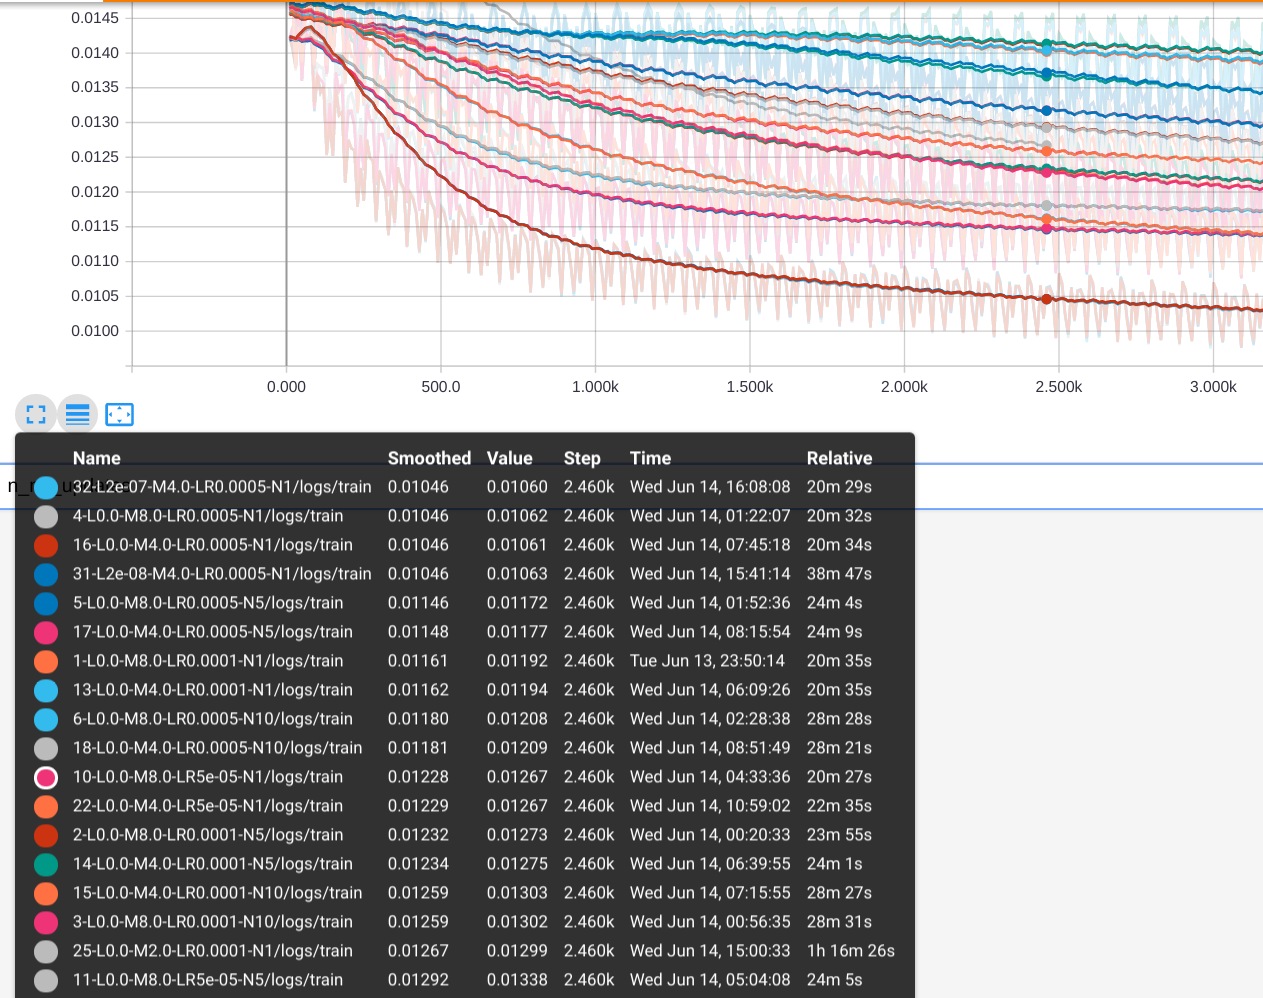
\includegraphics[width=4.6in]{dbm-mnist/lr_l2_maxnorm_10k.png}
\\[0.5em]
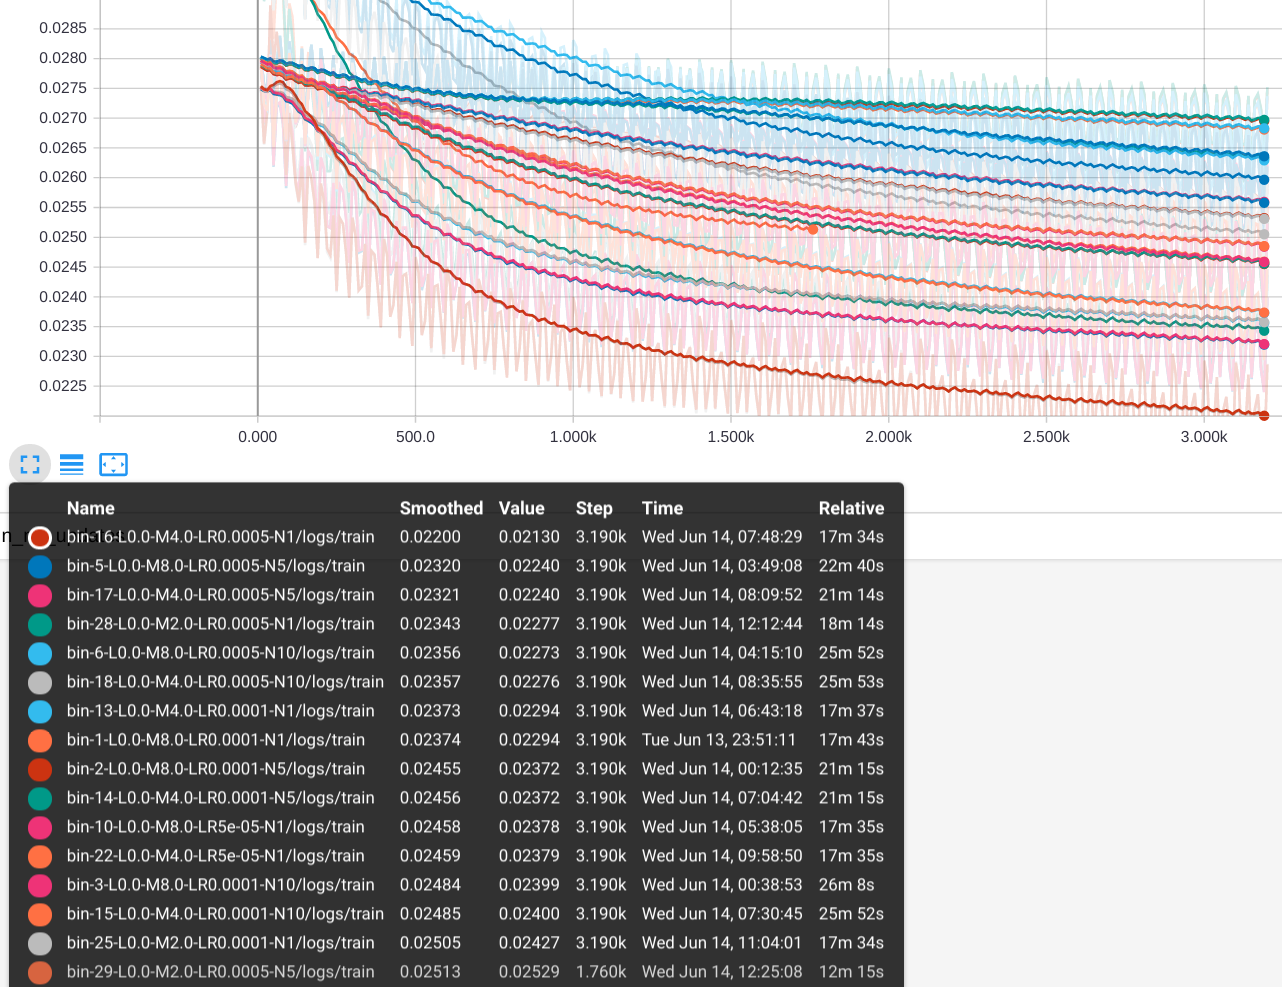
\includegraphics[width=4.6in]{dbm-mnist/l2_m_lr_n_bin_10k.png}
\caption{\emph{Top}: the effect of various choices of L2 weight decay coefficient, learning rate, maxnorm constraint and number of Gibbs steps on reconstruction error on random subset of 10k images from MNIST; 20 mean-filed updates, 100 particles, momentum $0.5\rightarrow 0.9$. \emph{Bottom}: the same, but on \u{binarized} version of MNIST, as suggested in \cite{goodfellow2012joint}.}
\end{mdframed}
\end{figure}

\clearpage

\begin{figure}[h]
\begin{mdframed}
\centering
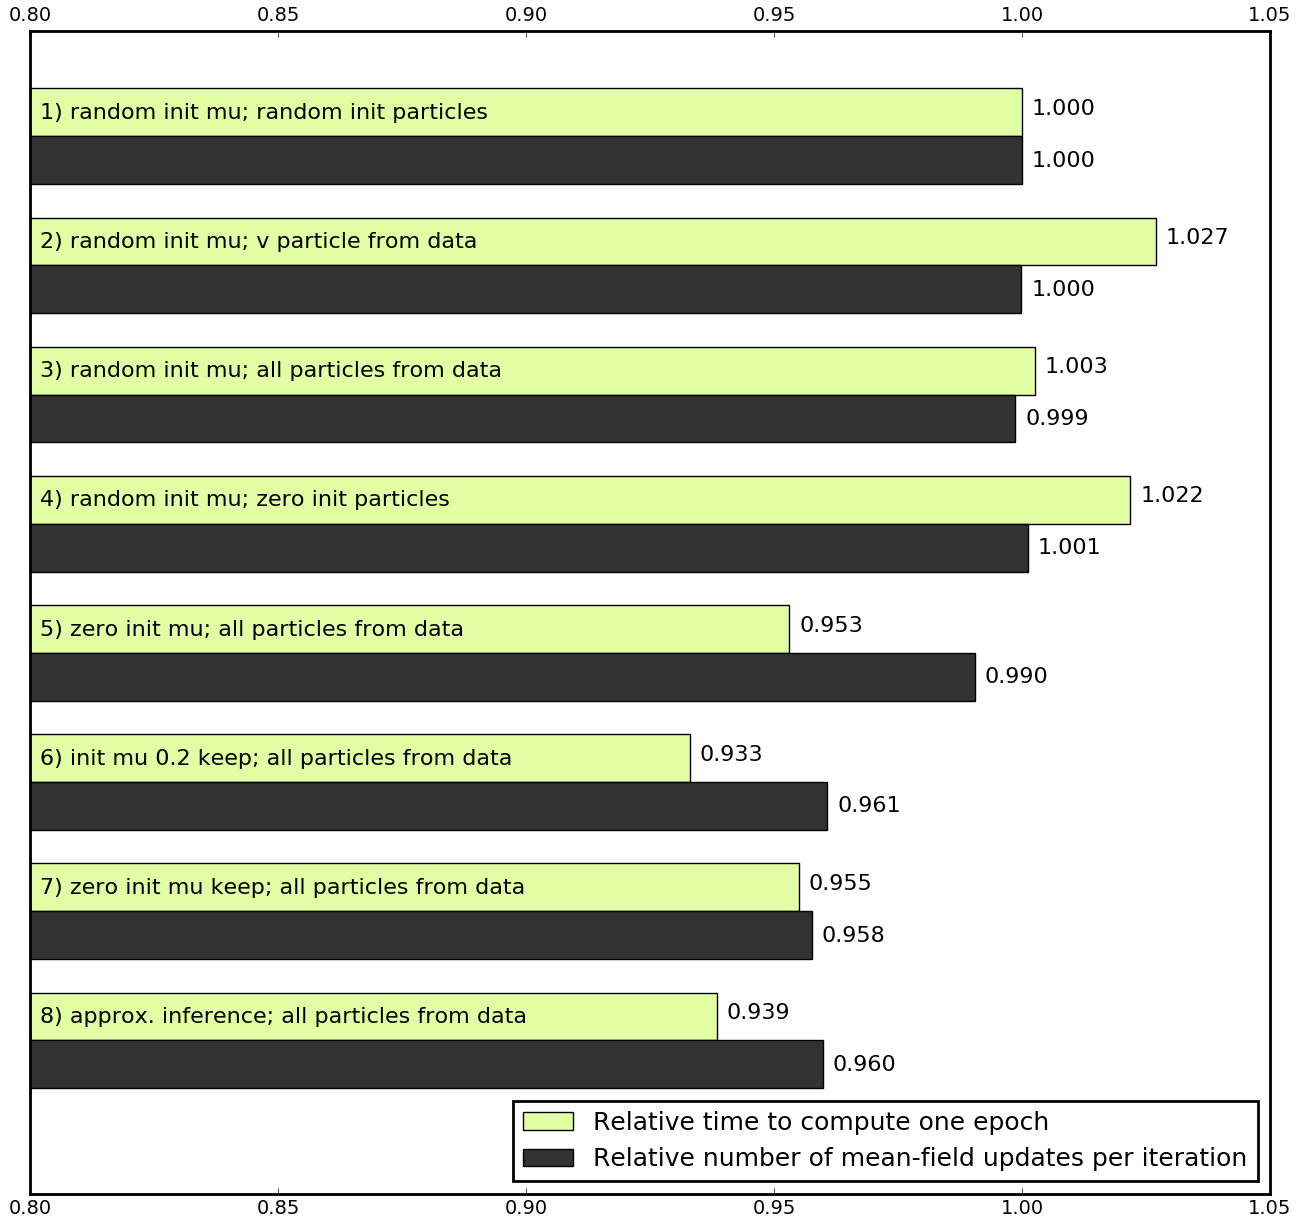
\includegraphics[width=3in]{dbm-mnist/mf_approaches.png}
\quad
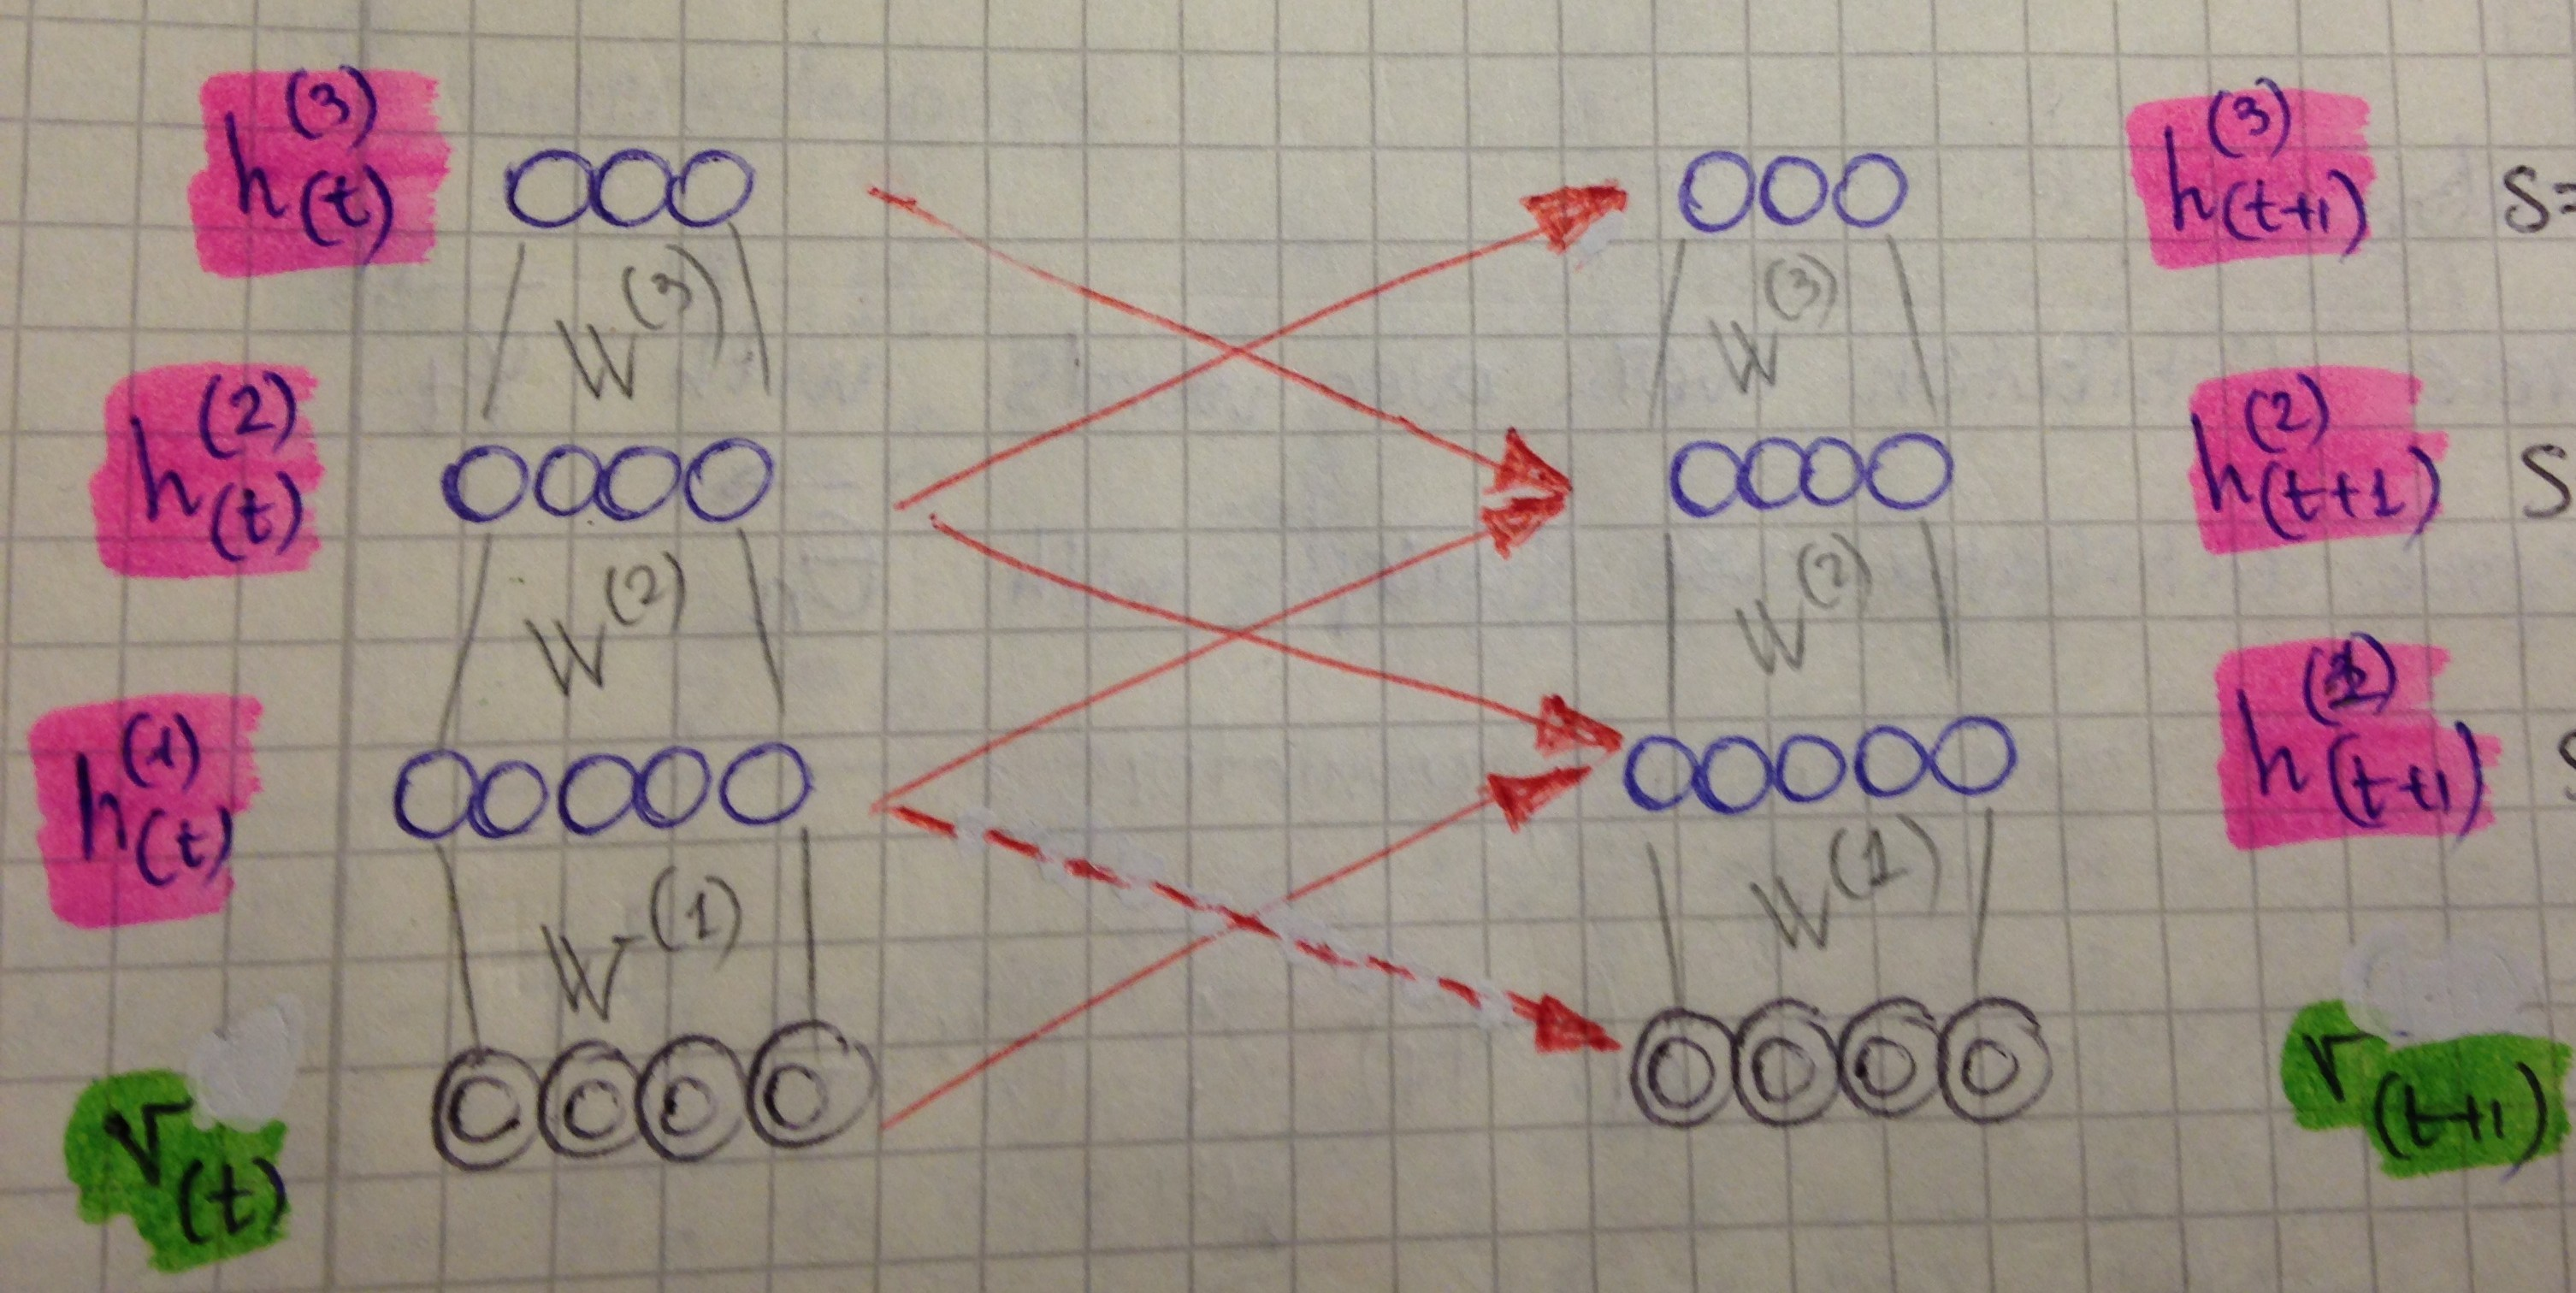
\includegraphics[width=2.5in]{dbm-mnist/parallel_gibbs.jpg}
\\[2em]
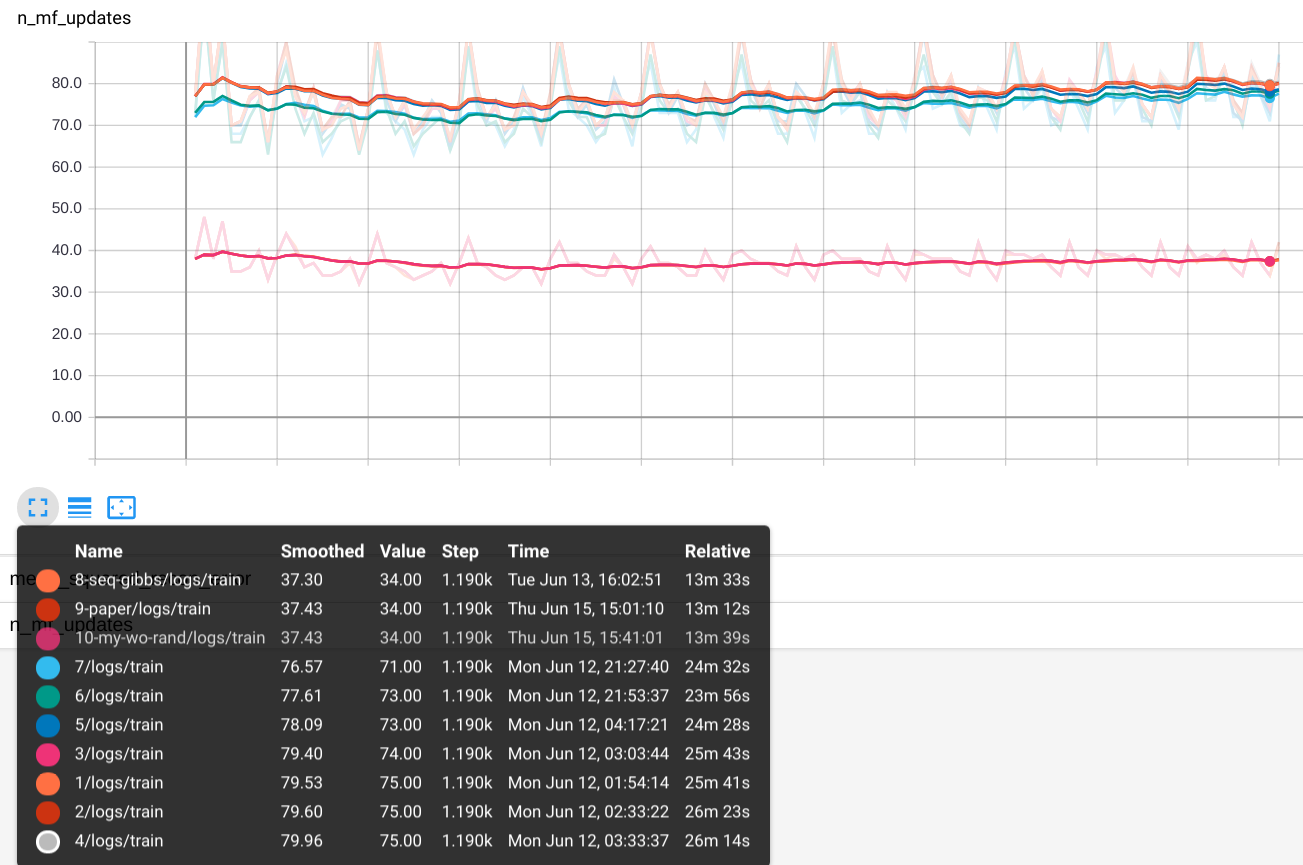
\includegraphics[width=4.5in]{dbm-mnist/n_mf_approaches.png}
\caption{\emph{Top left}: Various approaches on particles and variational parameters initialization to speedup mean-field convergence I've tried. Numbers of mean-filed updates are meant to achieve $10^{-11}$ tolerance. \tb{In sum}: it is always better to initialize \u{all} particles (including hidden ones) from the training data (hidden particles on the first level, for instance, should be initialized from the extracted fratures $\mb{q}_i=p(\mb{h}|\mb{v}=\mb{x}_i;\bs{\psi})$ from the first pre-trained RBM. Not resetting variation parameters between different gibbs updates is also slightly faster than bottom-up approximate inference described in \cite{salakhutdinov2009deep, salakhutdinov2010efficient}. It is thus a combination of these two best approaches (approx. inference + not resetting) is implemented in \texttt{DBM} class. Notwithstanding, the results (in terms of reconstruction error) were pretty robust to the exact number of mean-field updates: similar when used 10 or 25 mean-field updates. \emph{Top right}: I also tried "parallel" version of Gibbs sampling. One mean-field update was faster ($\approx 1.1-1.2$) but the total number of them was nearly twice as many. \emph{Bottom}: dynamics of mean field updates for various approaches. See also excel table. Experiments were tried on random subset 10k images.}
\end{mdframed}
\end{figure}

\clearpage

\begin{figure}[h]
\begin{mdframed}
\centering
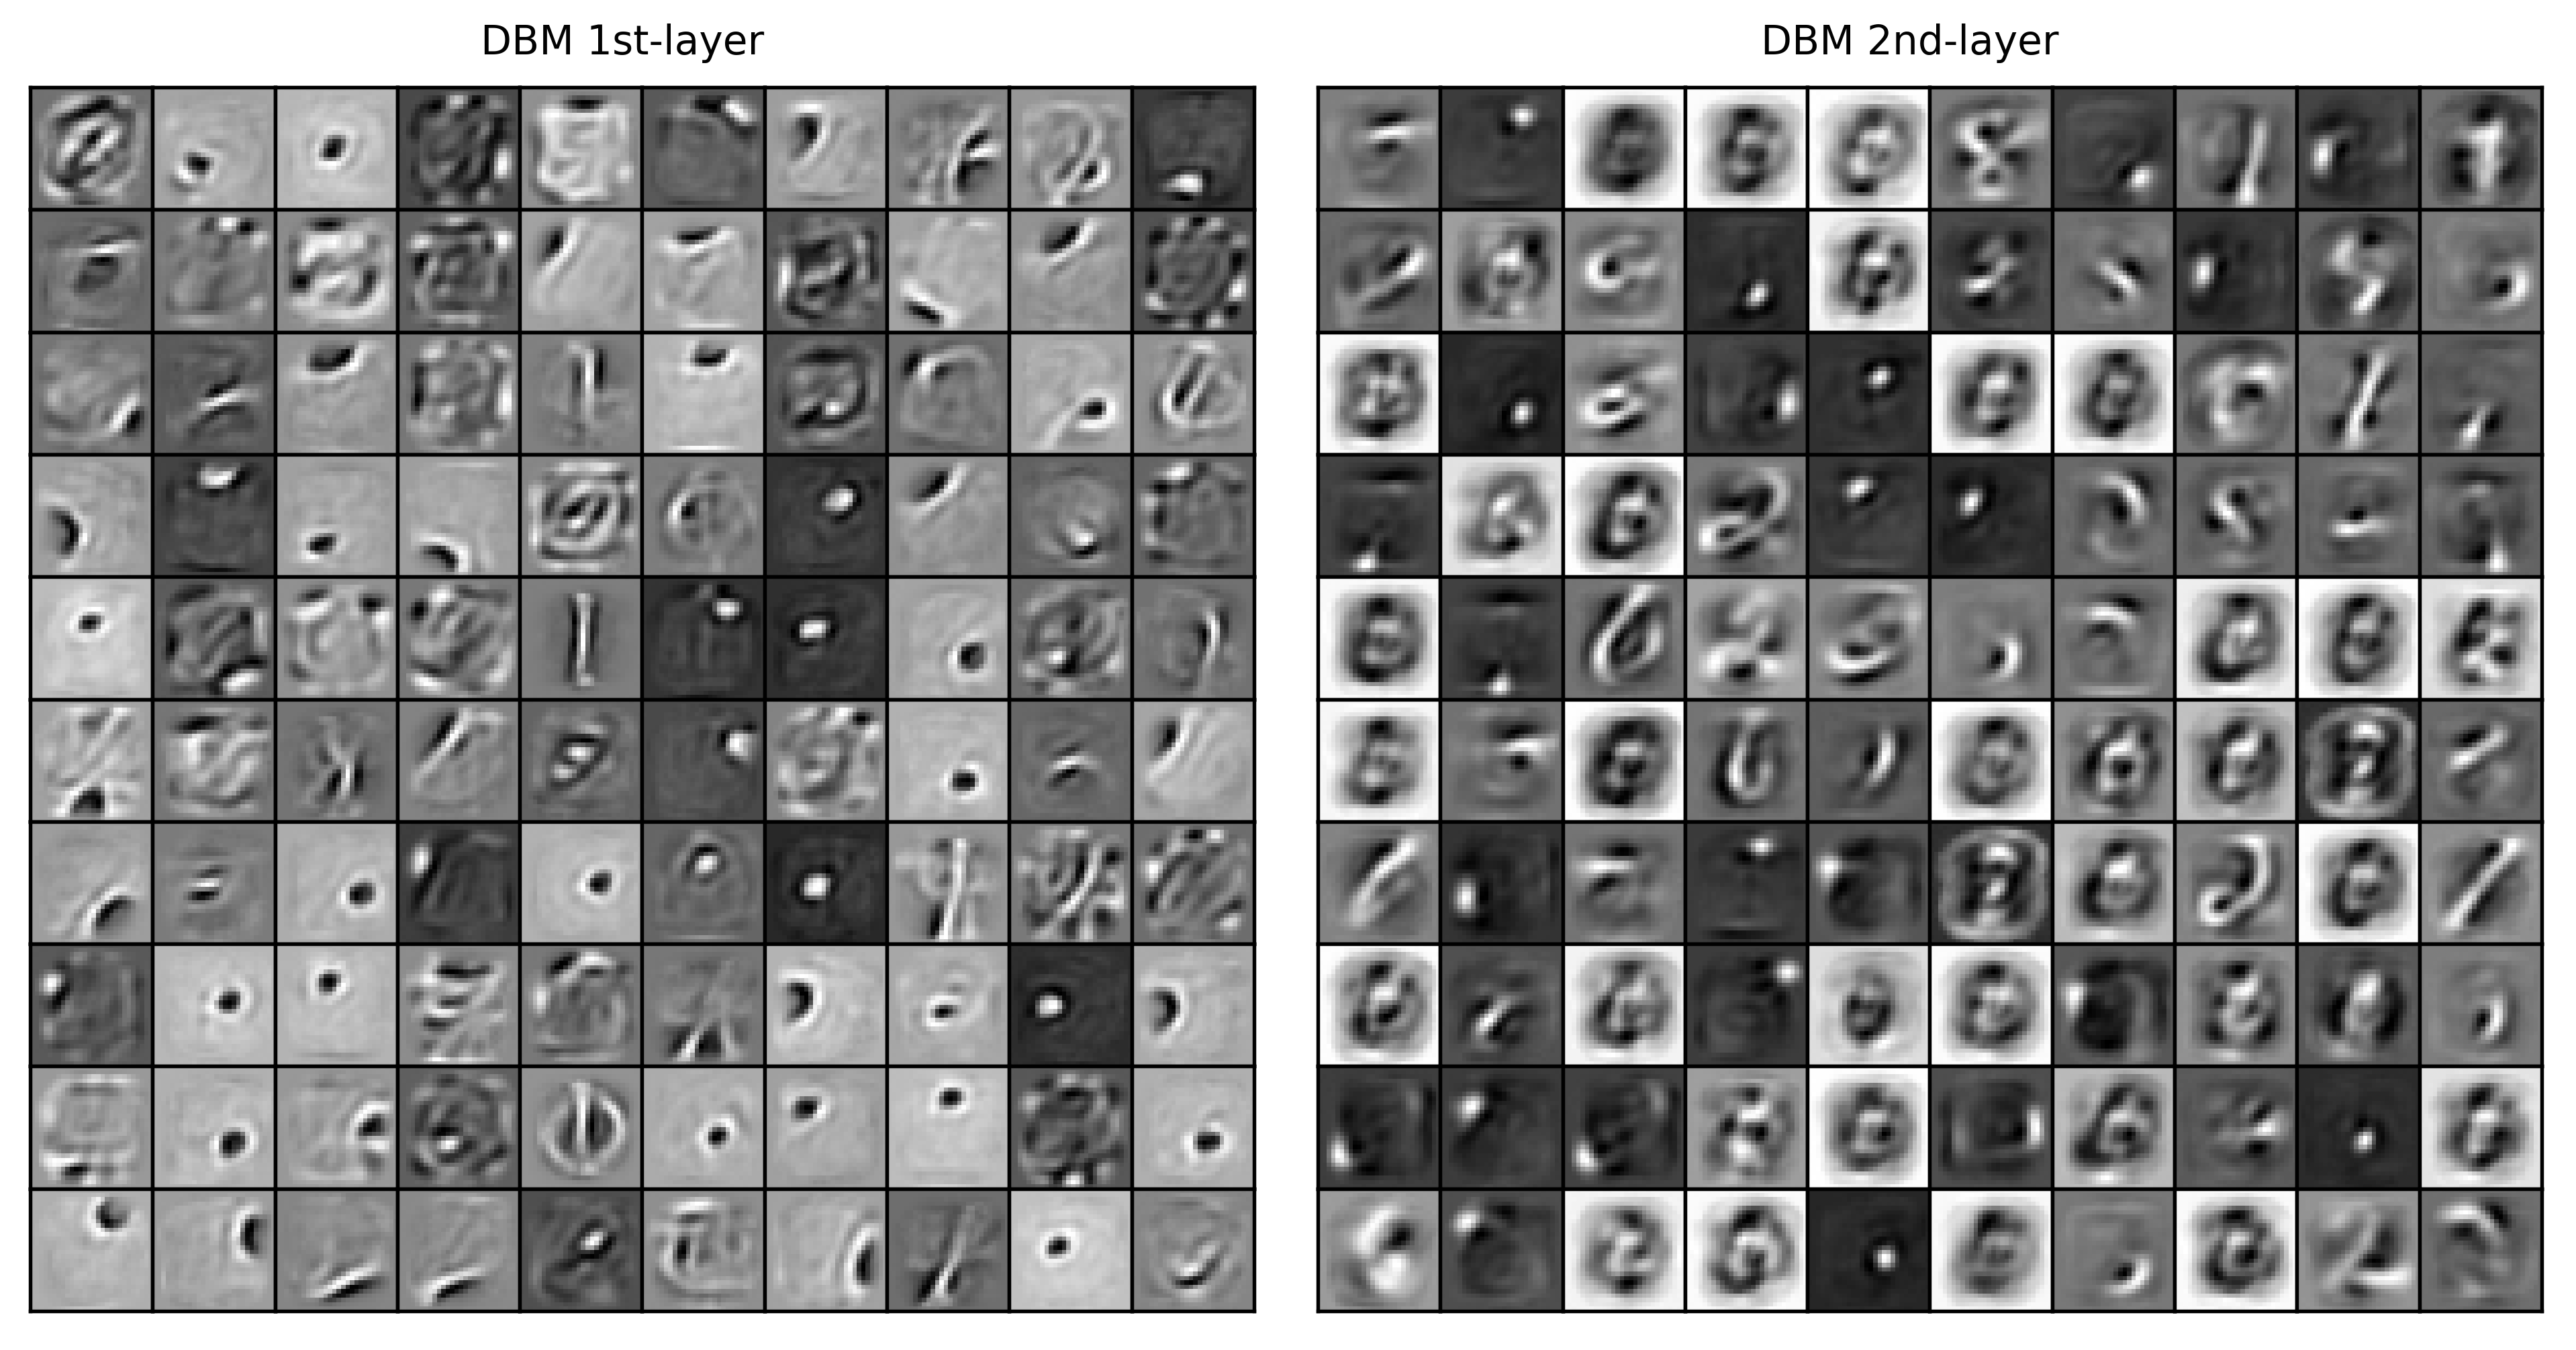
\includegraphics[width=5.6in]{dbm-mnist/filters.png}
\\[2em]
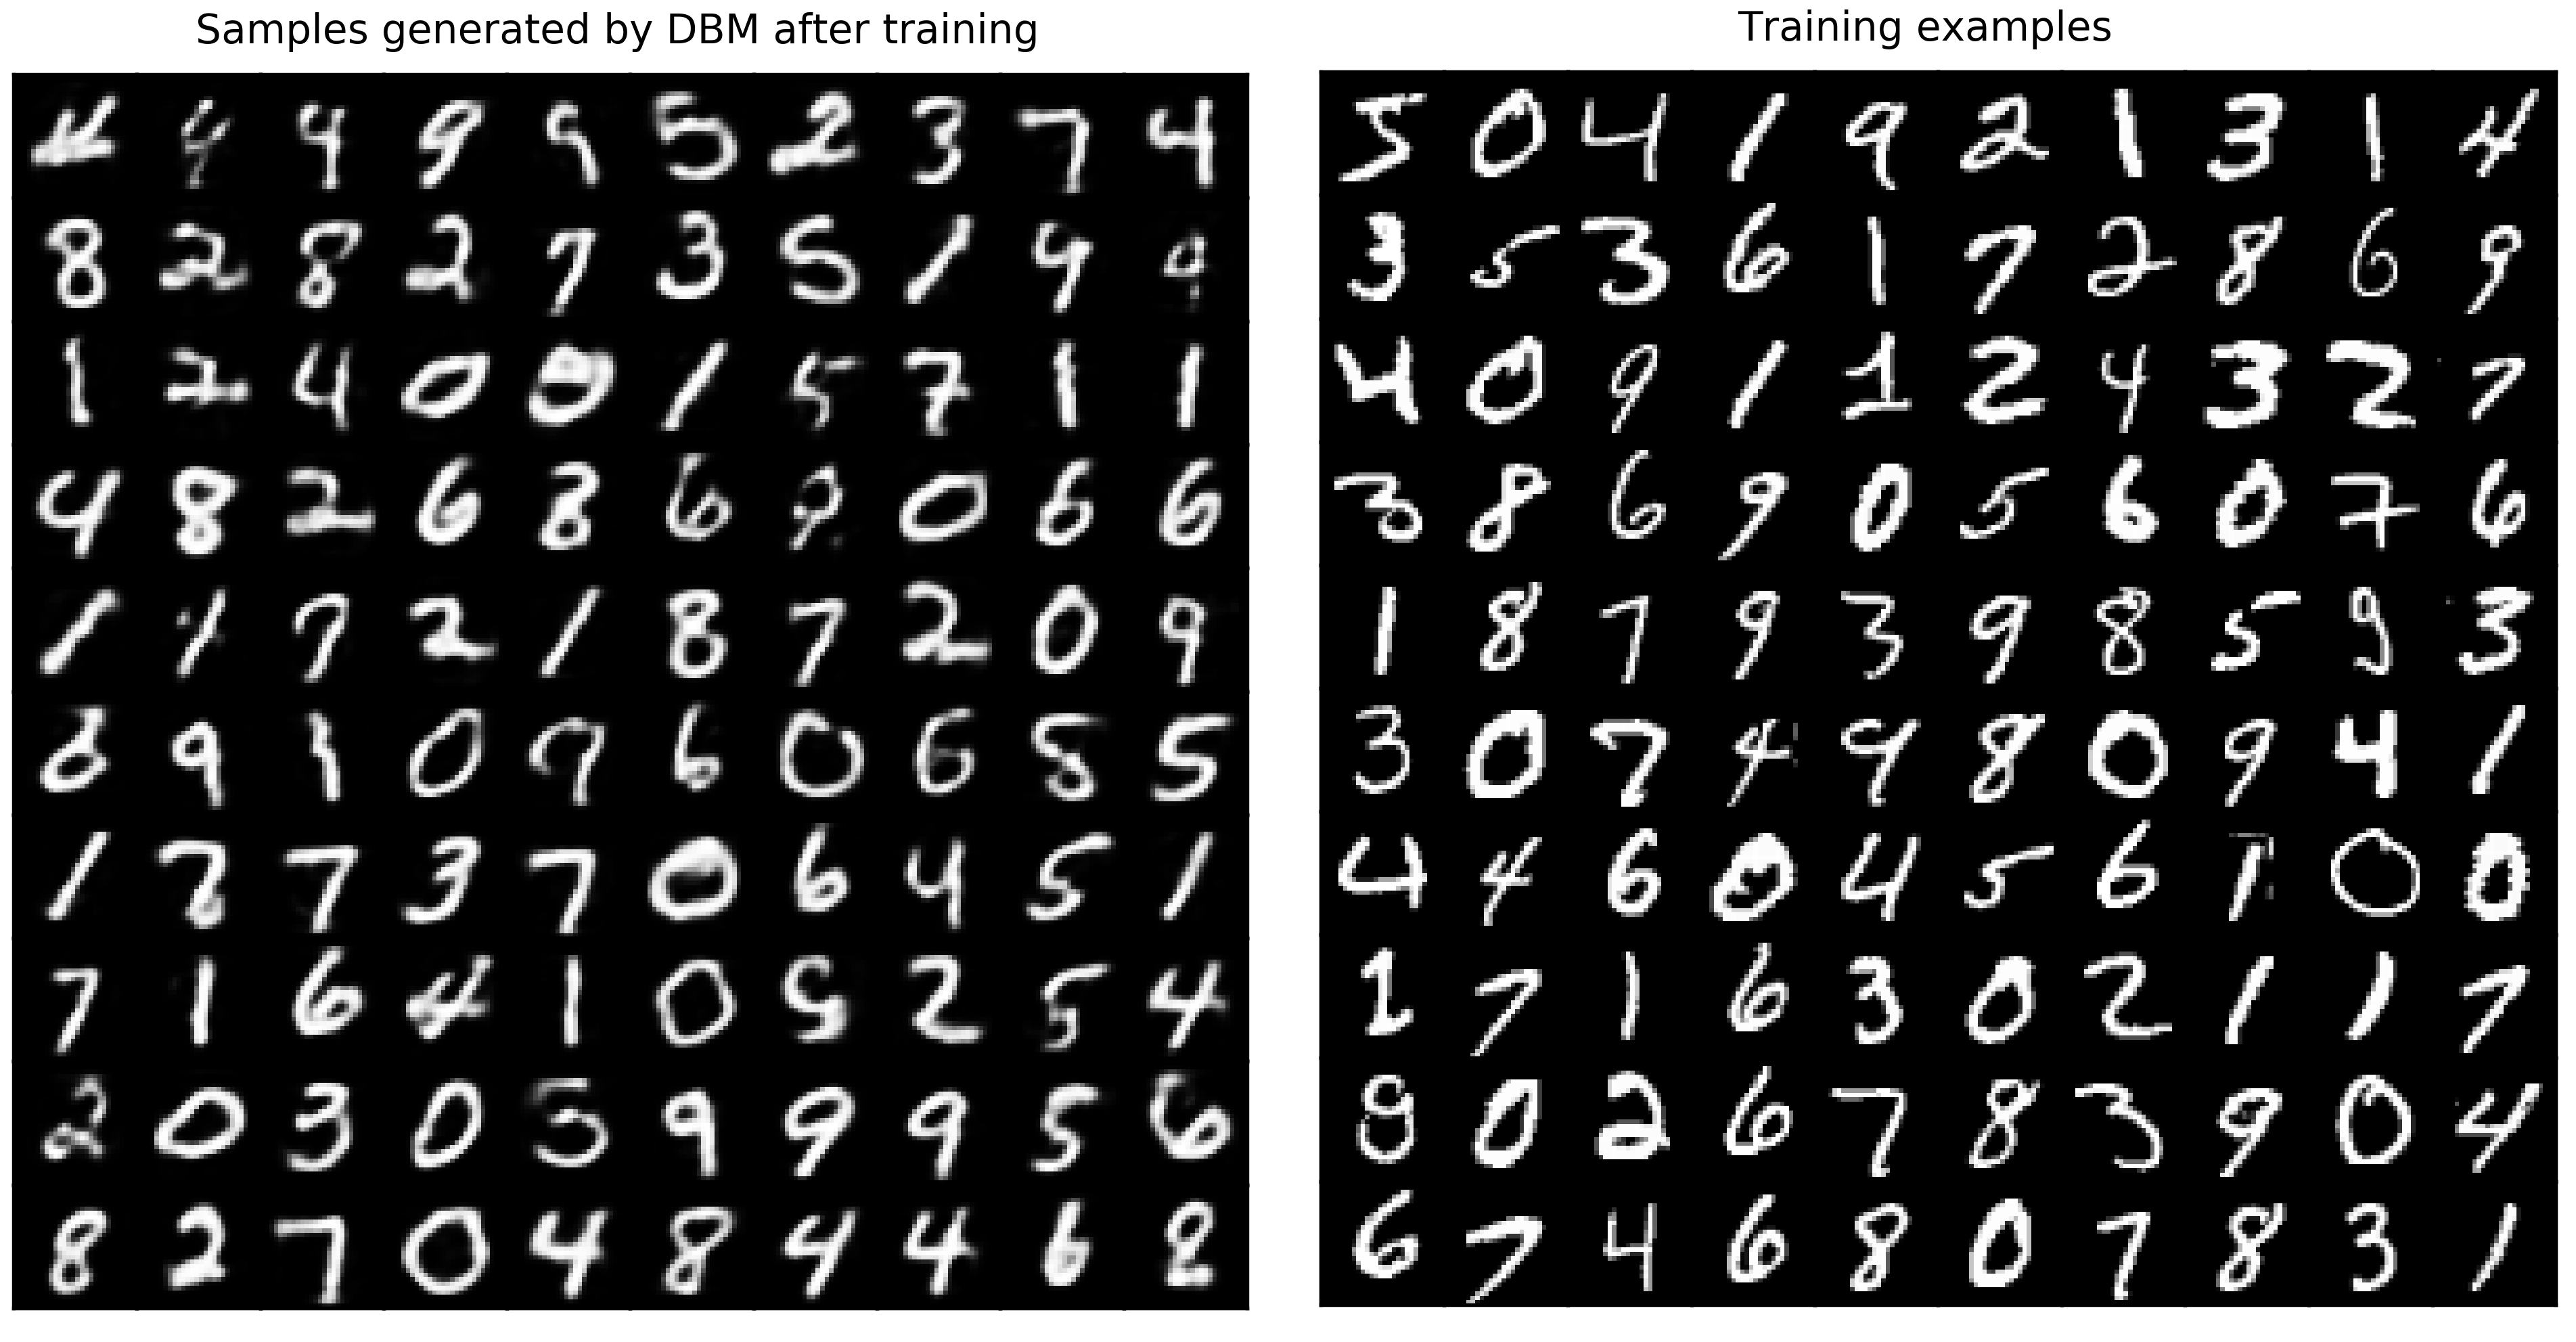
\includegraphics[width=5.6in]{dbm-mnist/samples.png}
\caption{Best model trained on full MNIST in this phase in terms of the generated samples quality. 2nd layer filters are visualized using method of \emph{weighted linear combinations} \cite{erhan2009visualizing}. \tb{\emph{Hyperparams}}: 100 particles, 25 mean-filed updates, 1 Gibbs step per iter, mean-field tolerance $10^{-7}$, momentum $0.5\rightarrow 0.9$, learning rate $5\cdot10^{-4}\rightarrow 10^{-5}$ by dividing by $(1.000015)^{600}$ each epoch, 200 epochs, batch-size 100, L2 $=10^{-7}$, maxnorm $=4$; sample all visible and hidden states.
}
\end{mdframed}
\end{figure}

\clearpage

\begin{figure}[h]
\begin{mdframed}
\centering
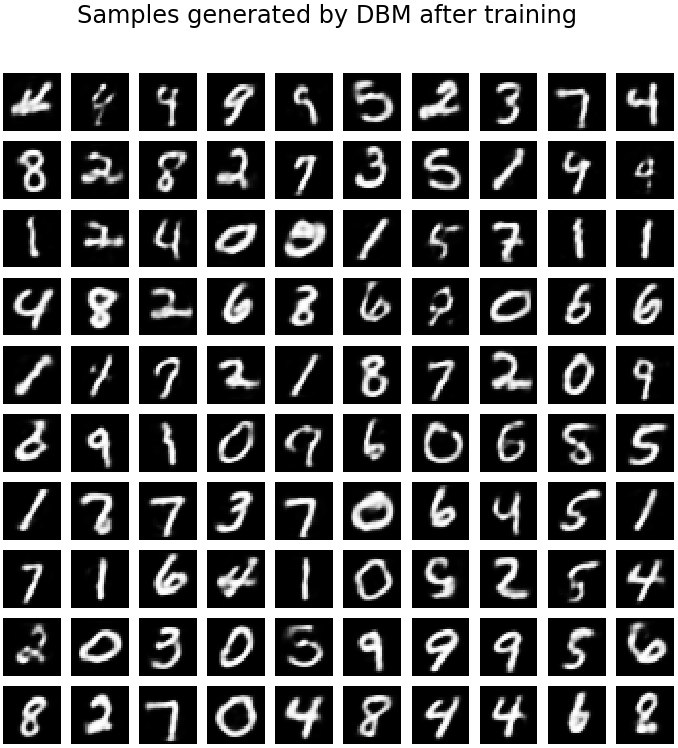
\includegraphics[width=2in]{dbm-mnist/samples_0k.png}
\quad
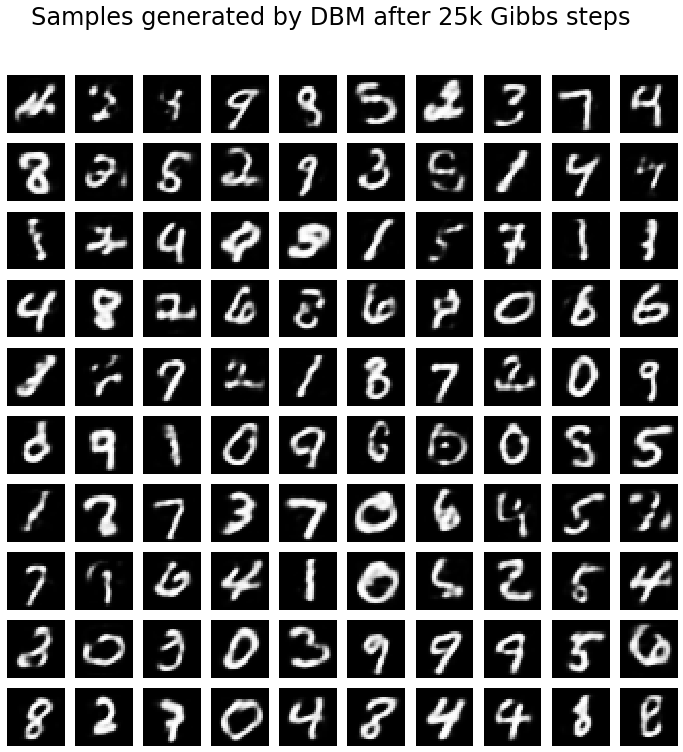
\includegraphics[width=2in]{dbm-mnist/samples_25k.png}
\quad
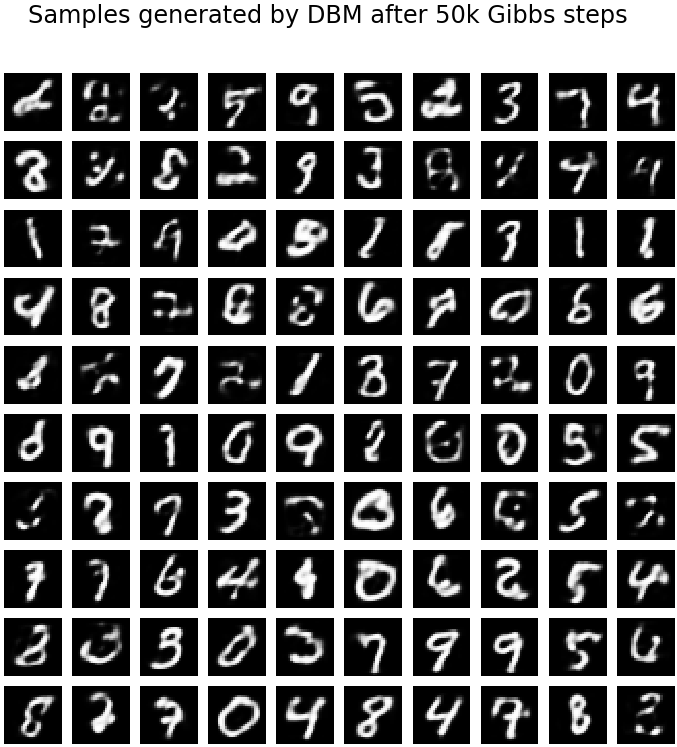
\includegraphics[width=2in]{dbm-mnist/samples_50k.png}
\\[2em]
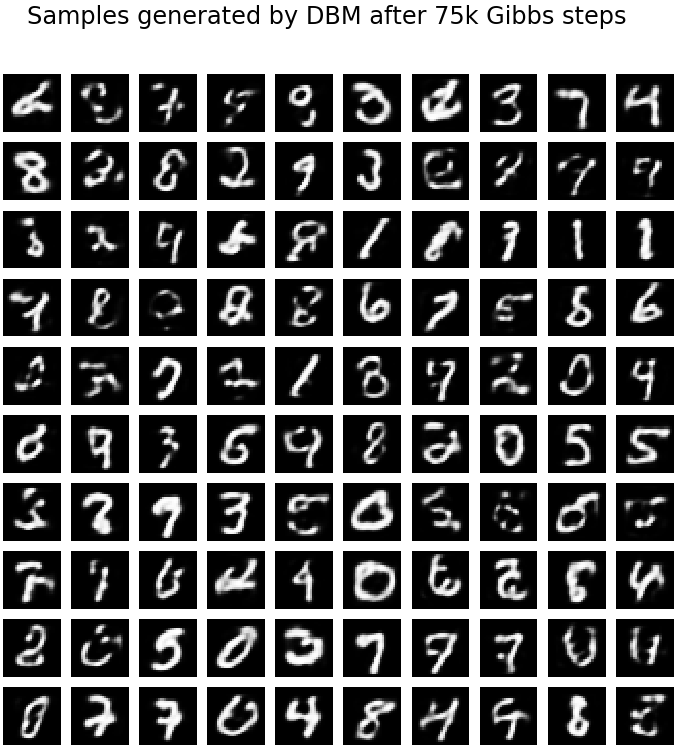
\includegraphics[width=2in]{dbm-mnist/samples_75k.png}
\quad
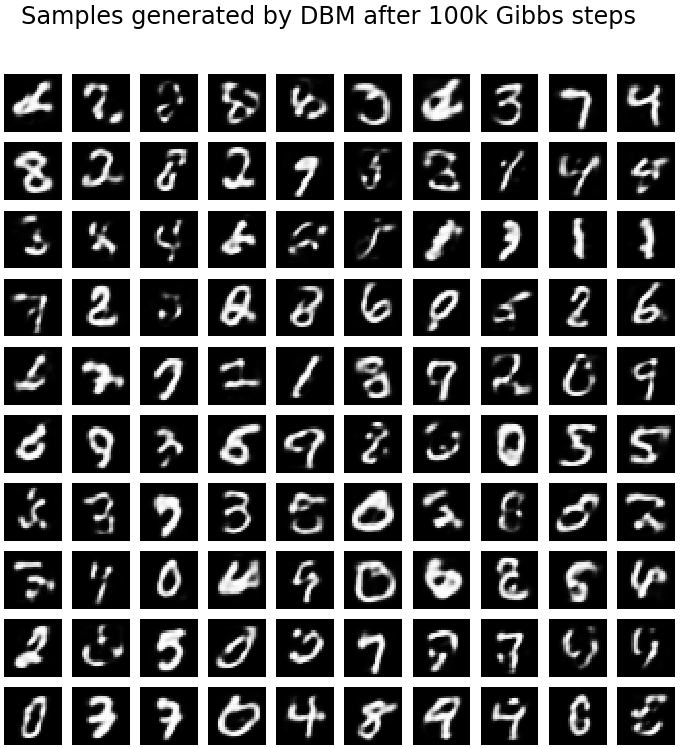
\includegraphics[width=2in]{dbm-mnist/samples_100k.png}
\quad
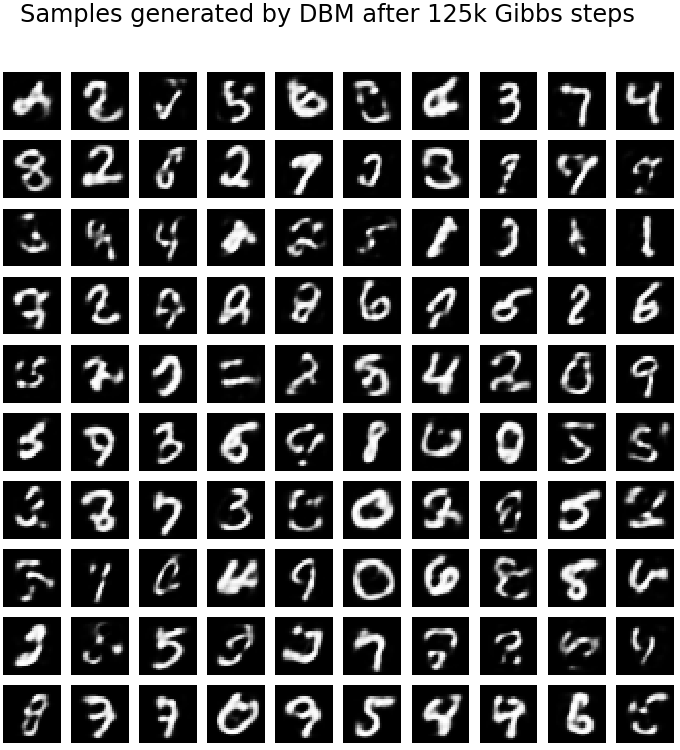
\includegraphics[width=2in]{dbm-mnist/samples_125k.png}
\\[2em]
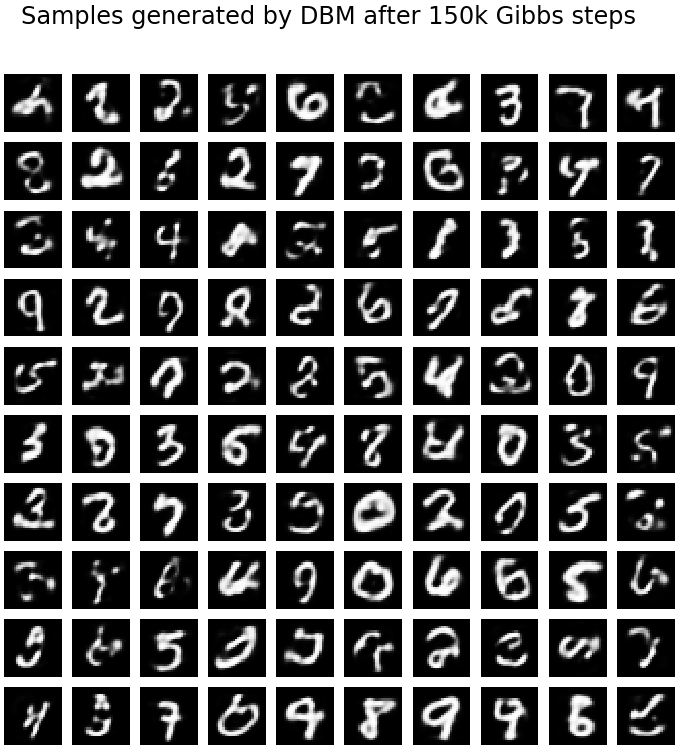
\includegraphics[width=2in]{dbm-mnist/samples_150k.png}
\quad
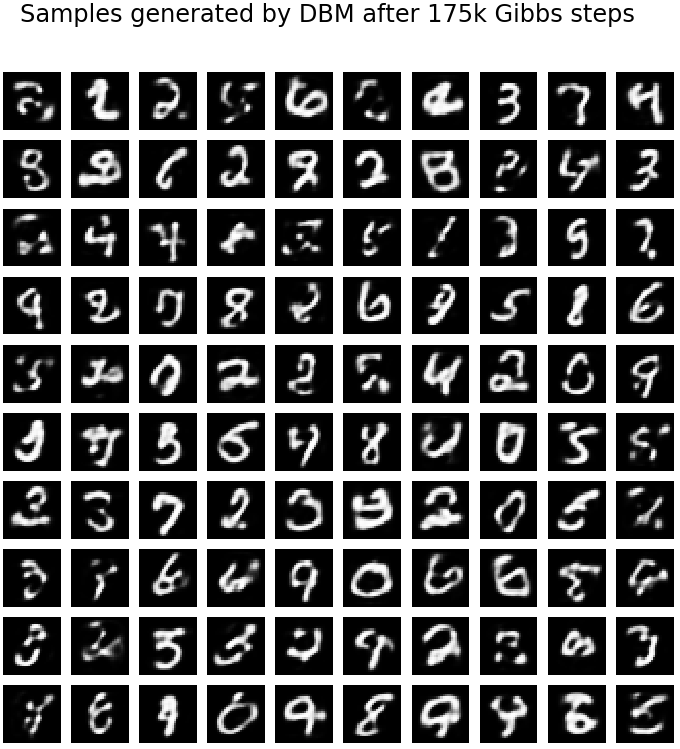
\includegraphics[width=2in]{dbm-mnist/samples_175k.png}
\quad
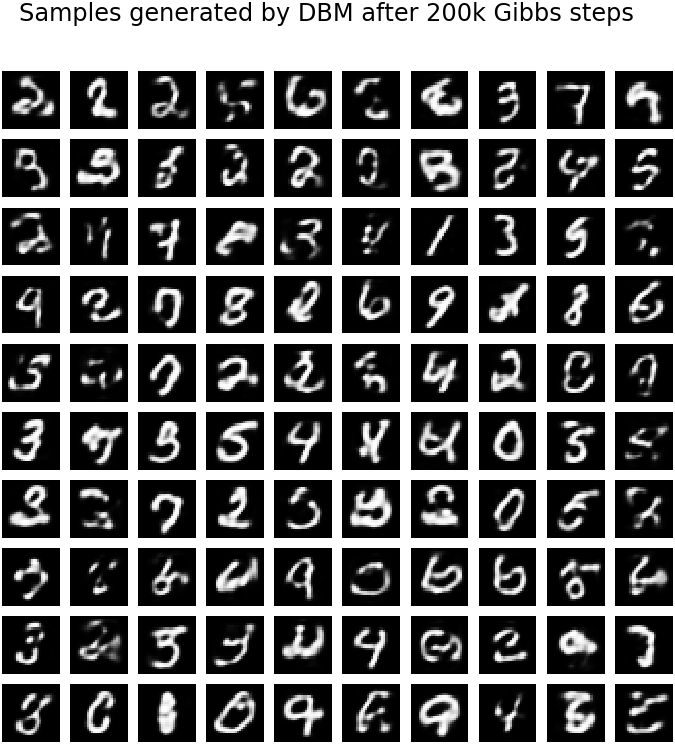
\includegraphics[width=2in]{dbm-mnist/samples_200k.png}
\caption{This illustrates how correlated generated samples are between one another because the approach used to generate them is MCMC-based one}.
\end{mdframed}
\end{figure}

\clearpage
\subsubsection{After sparsity targets, AIS are implemented}
After AIS is implemented, now it is possible to quantitatively evaluate DBM performance. To do this, I cross-validated 216 models with various hyperparameters on small held-out validation set $\rightarrow$ chose best values of hyperparameters based on ELBO estimation and quality of samples $\rightarrow$ repeated for 54 models with larger validation set $\rightarrow$ 4 $\rightarrow$ 1.
\\
\tb{Interesting observation}: AIS is (much) more accurate for better models and which are trained longer.
Results:

\begin{figure}[h]
\begin{mdframed}
\centering
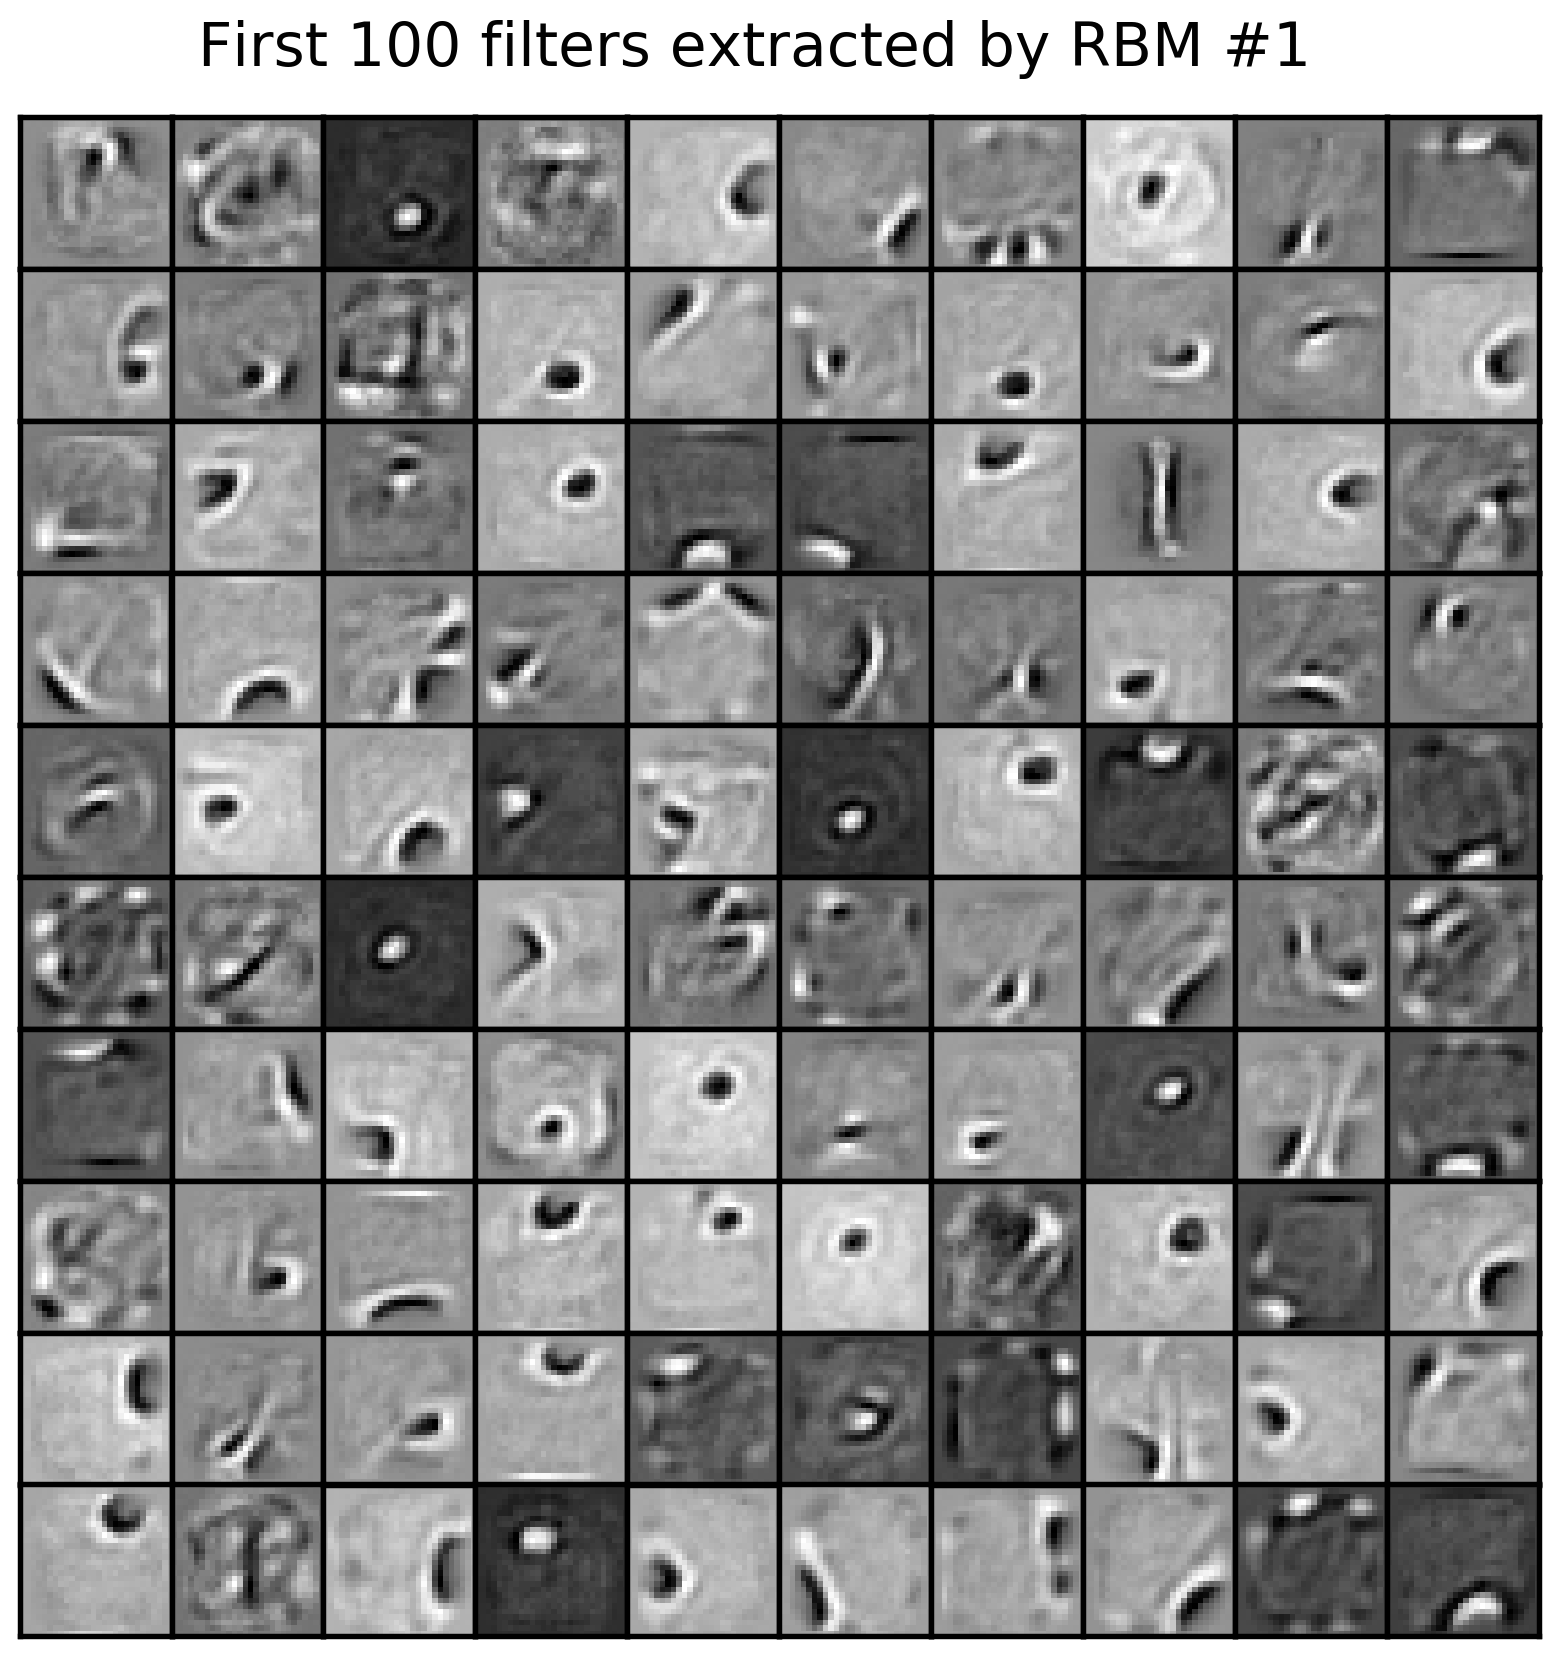
\includegraphics[width=2.5in]{dbm-mnist-latest/rbm1.png}
\quad
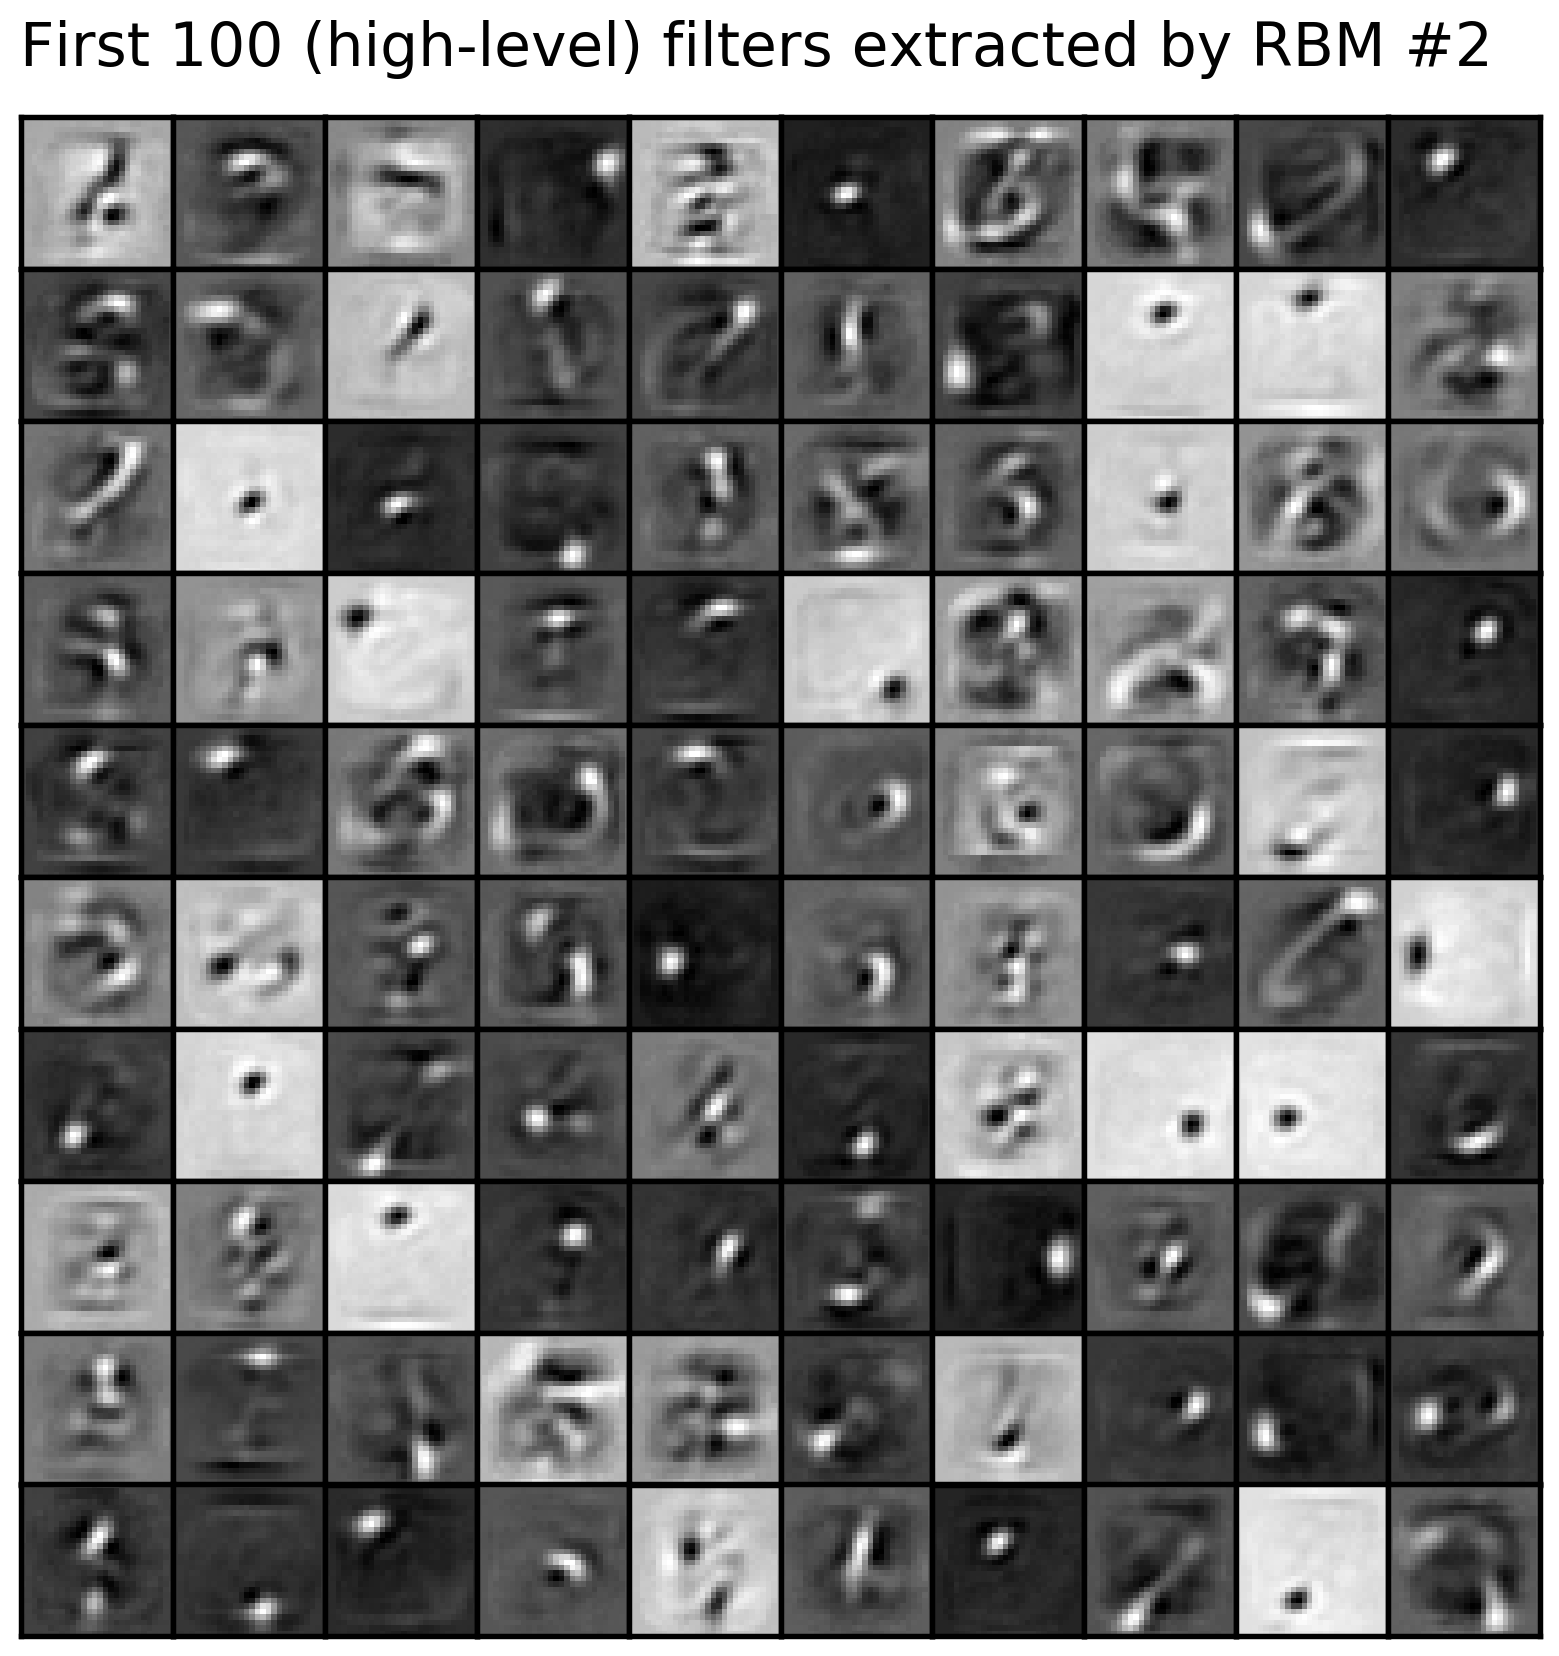
\includegraphics[width=2.5in]{dbm-mnist-latest/rbm2.png}
\\[2em]
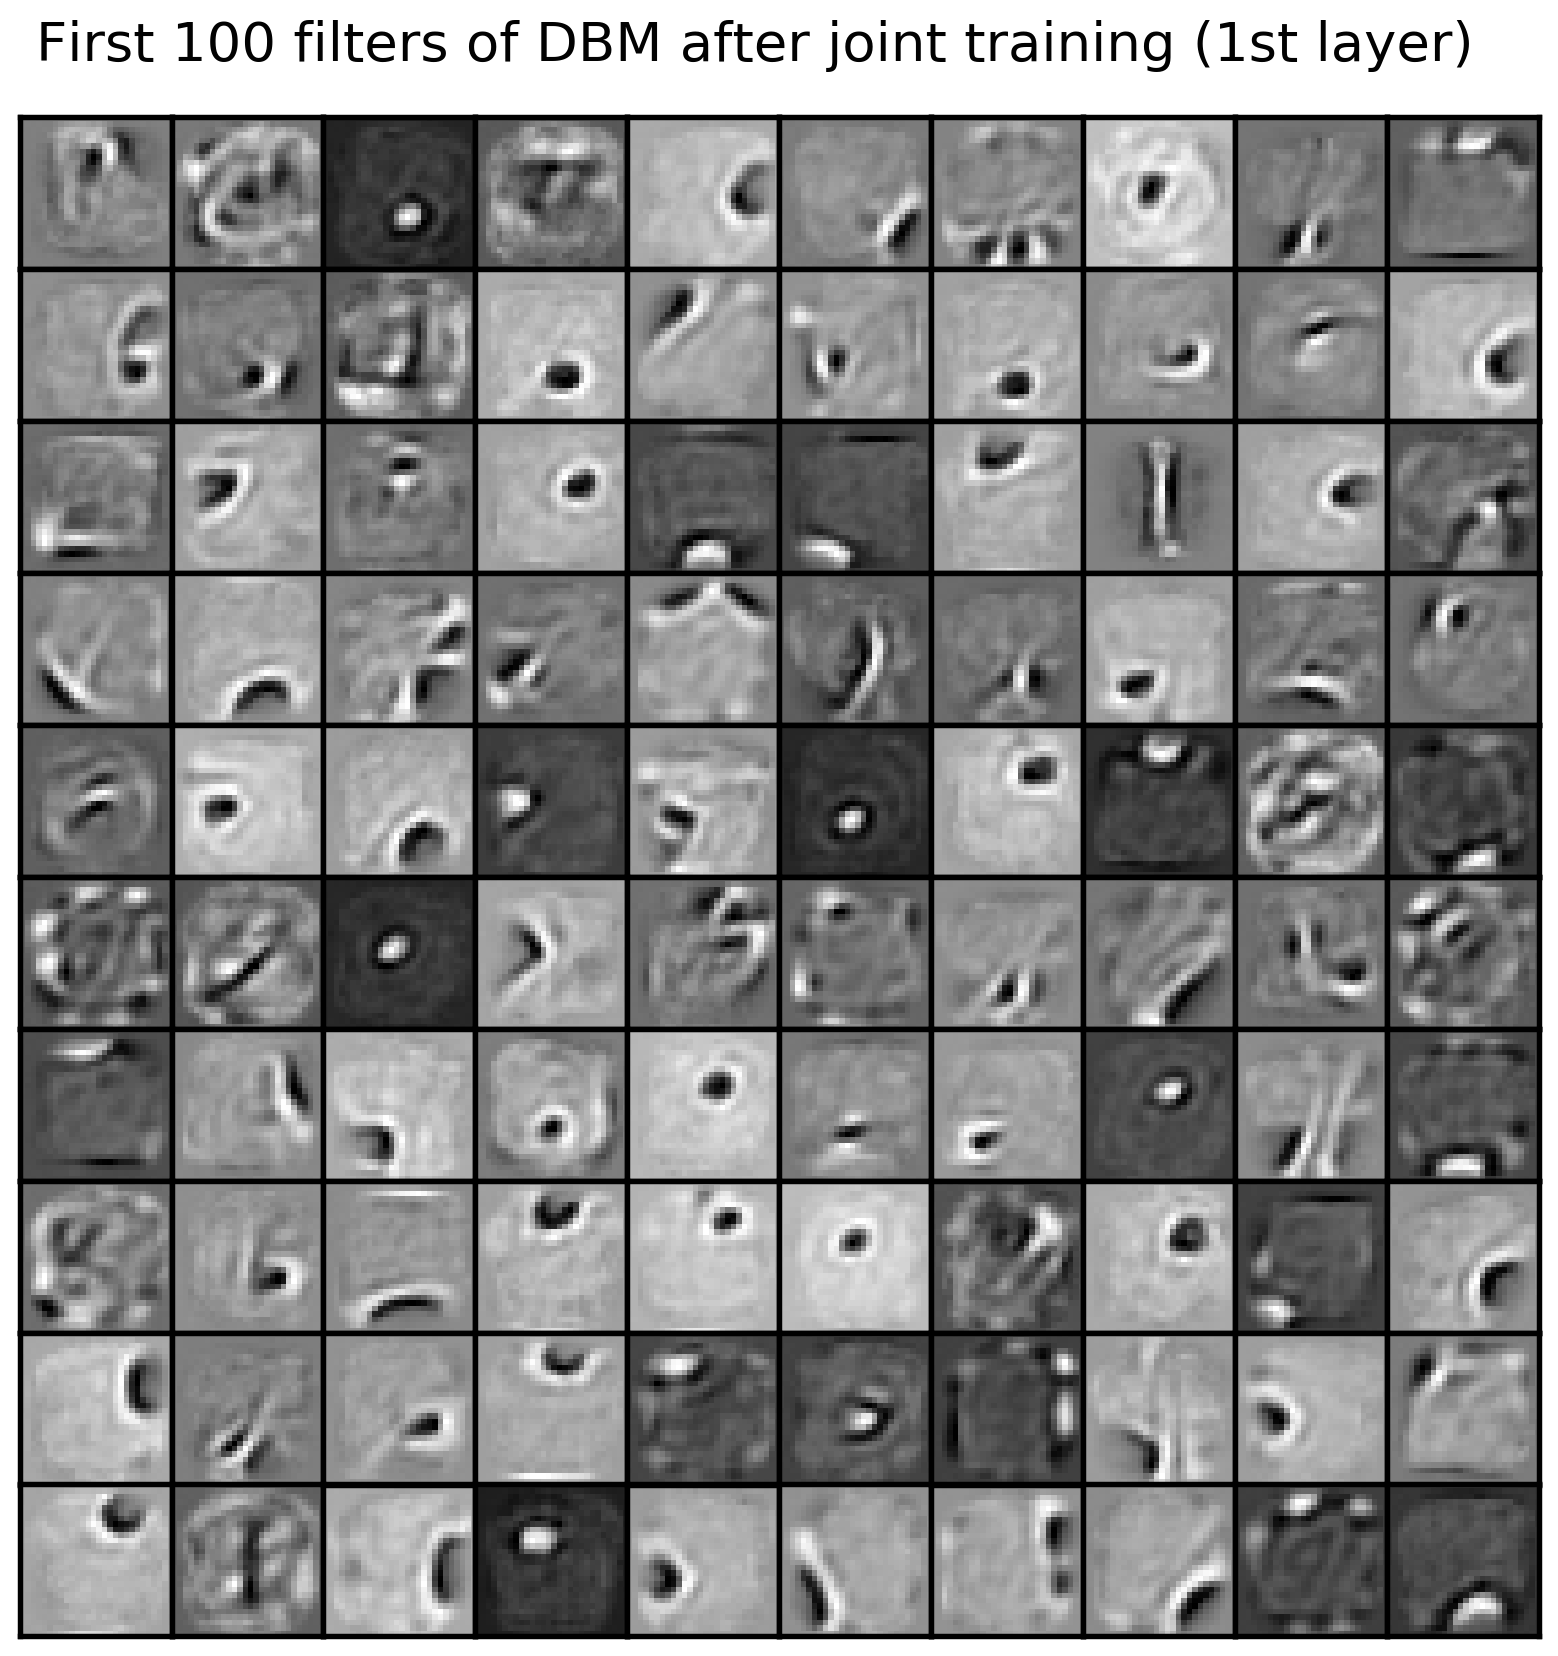
\includegraphics[width=2.5in]{dbm-mnist-latest/W1_joint.png}
\quad
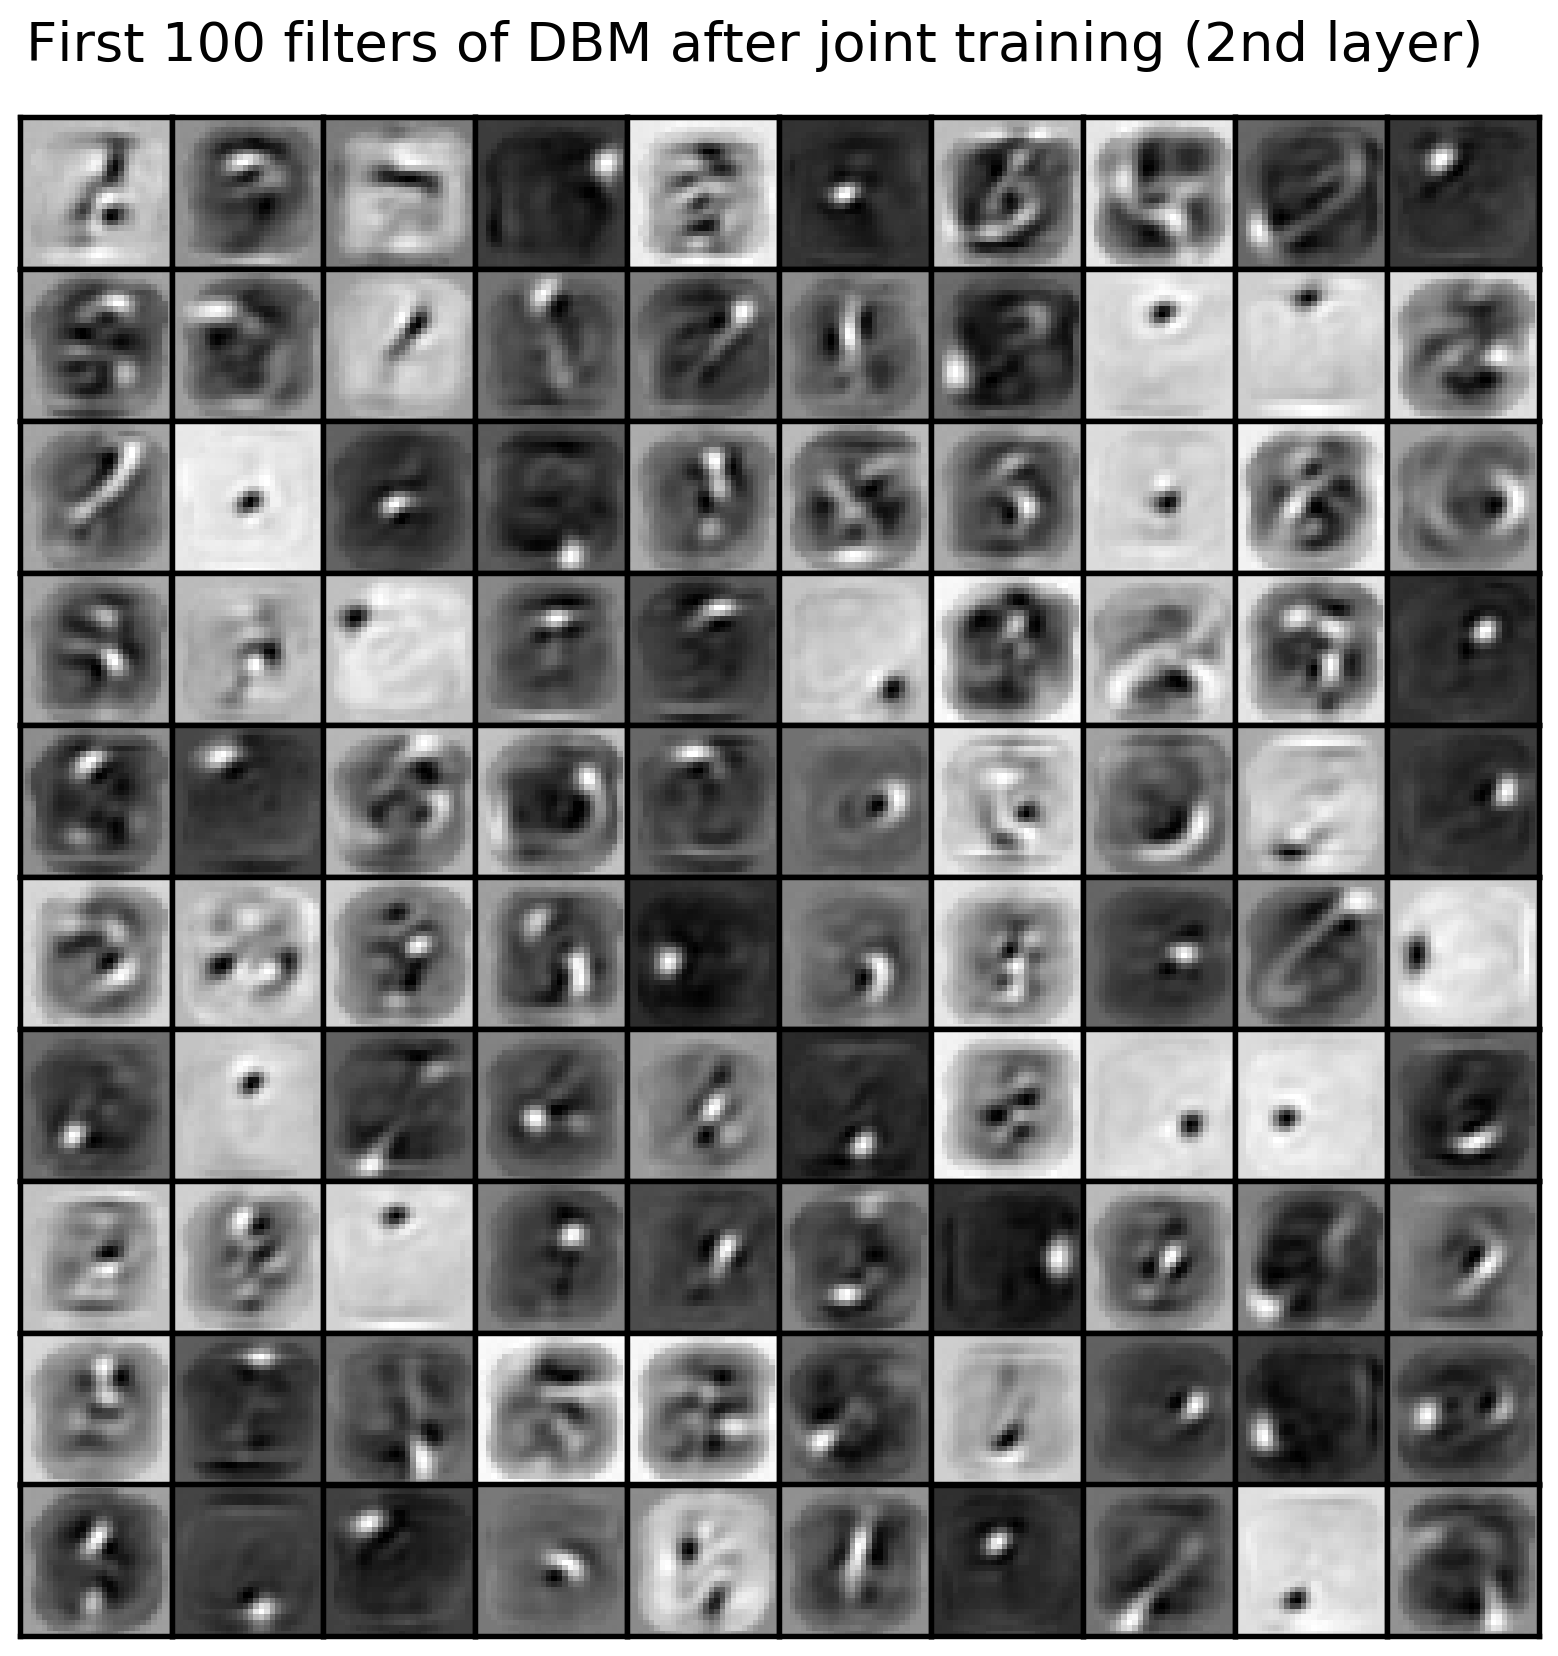
\includegraphics[width=2.5in]{dbm-mnist-latest/W2_joint.png}
\caption{Weight filters}.
\end{mdframed}
\end{figure}

\clearpage
\begin{figure}[h]
\begin{mdframed}
\centering
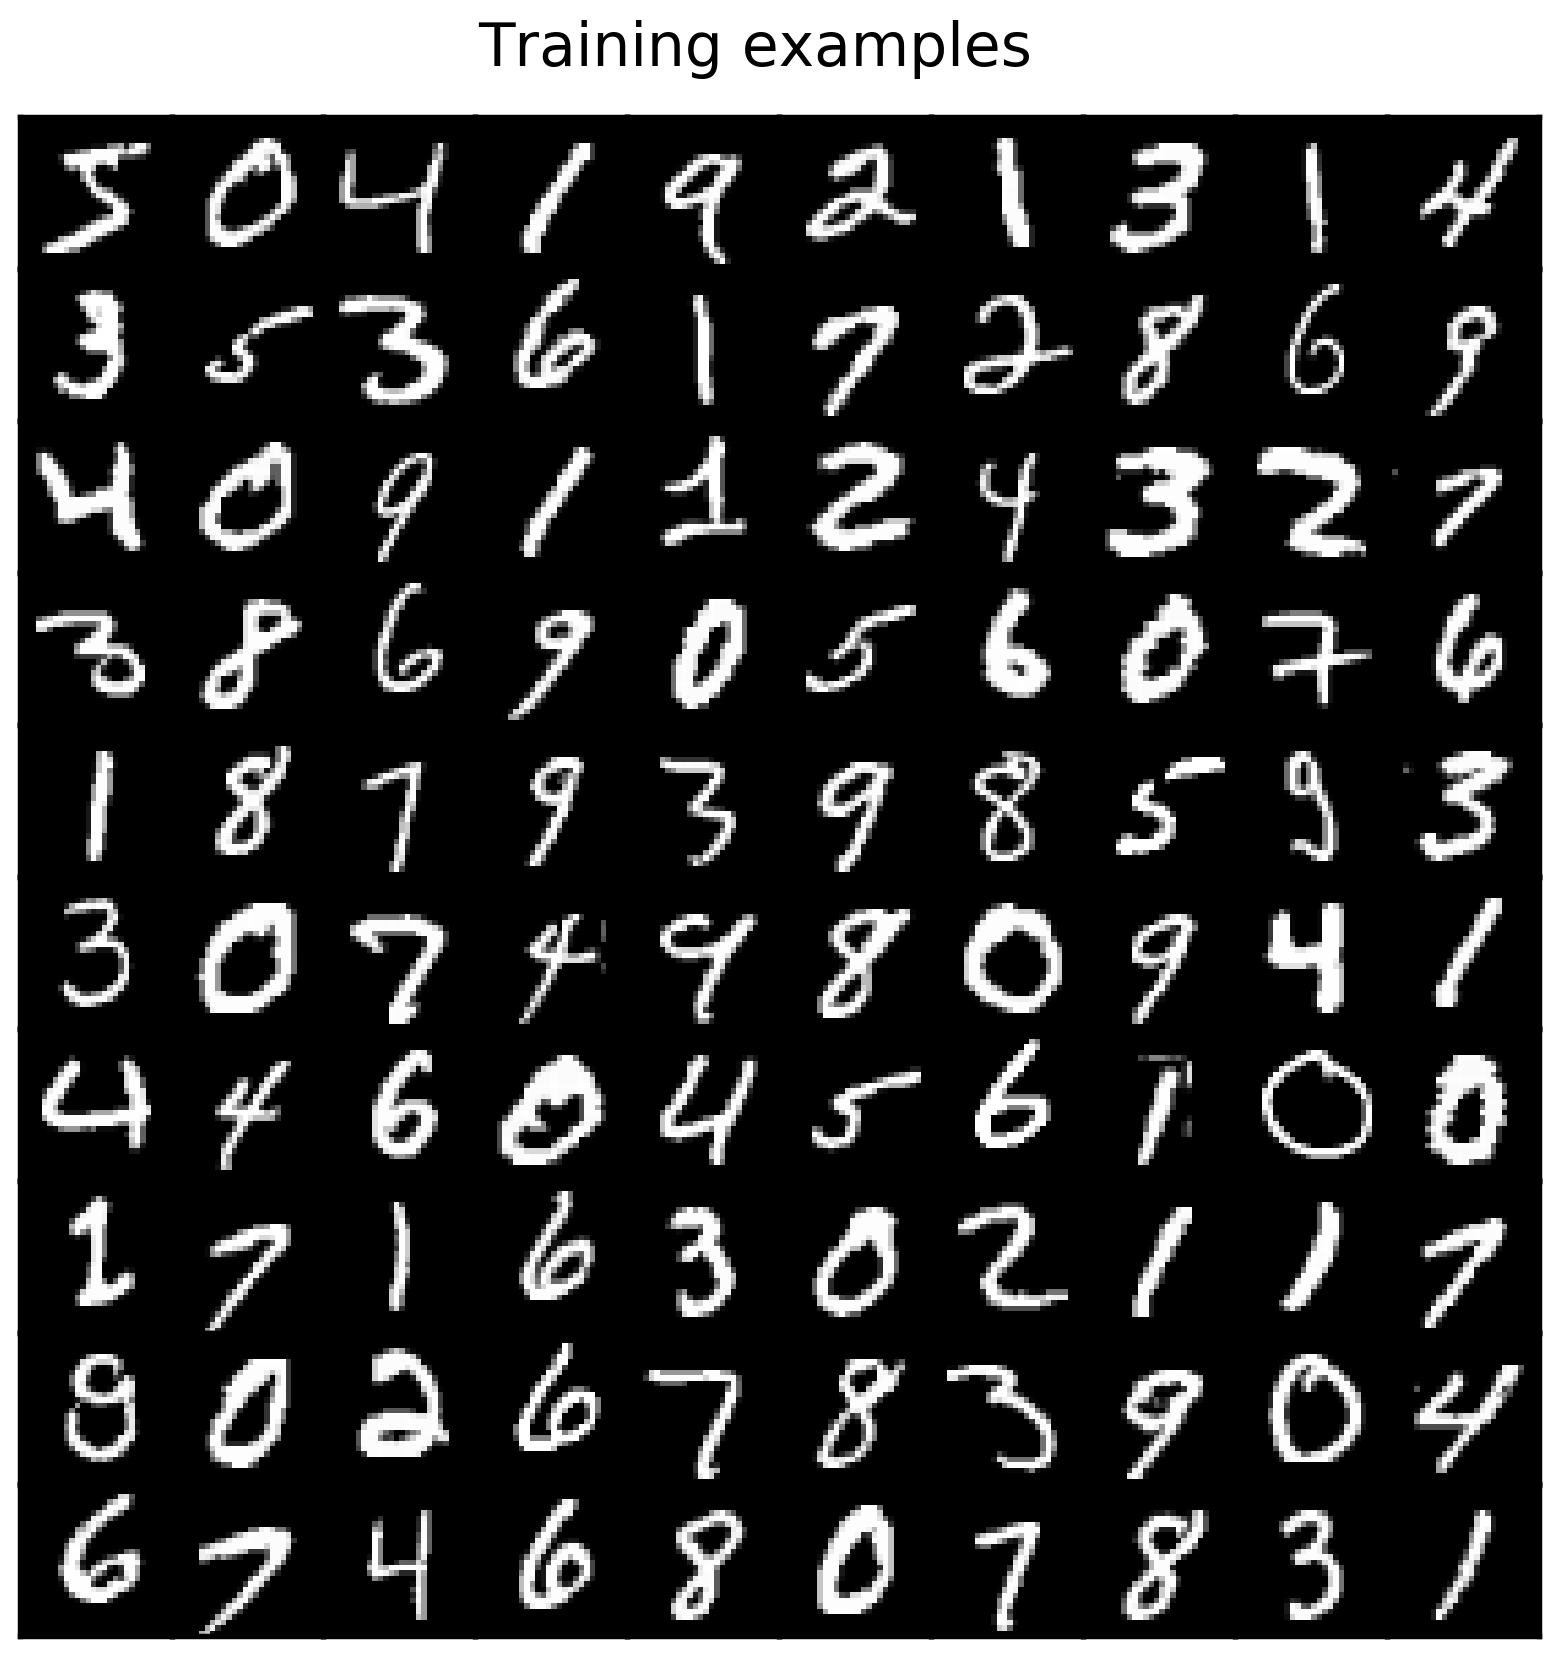
\includegraphics[width=2.8in]{dbm-mnist-latest/mnist.png}
\quad
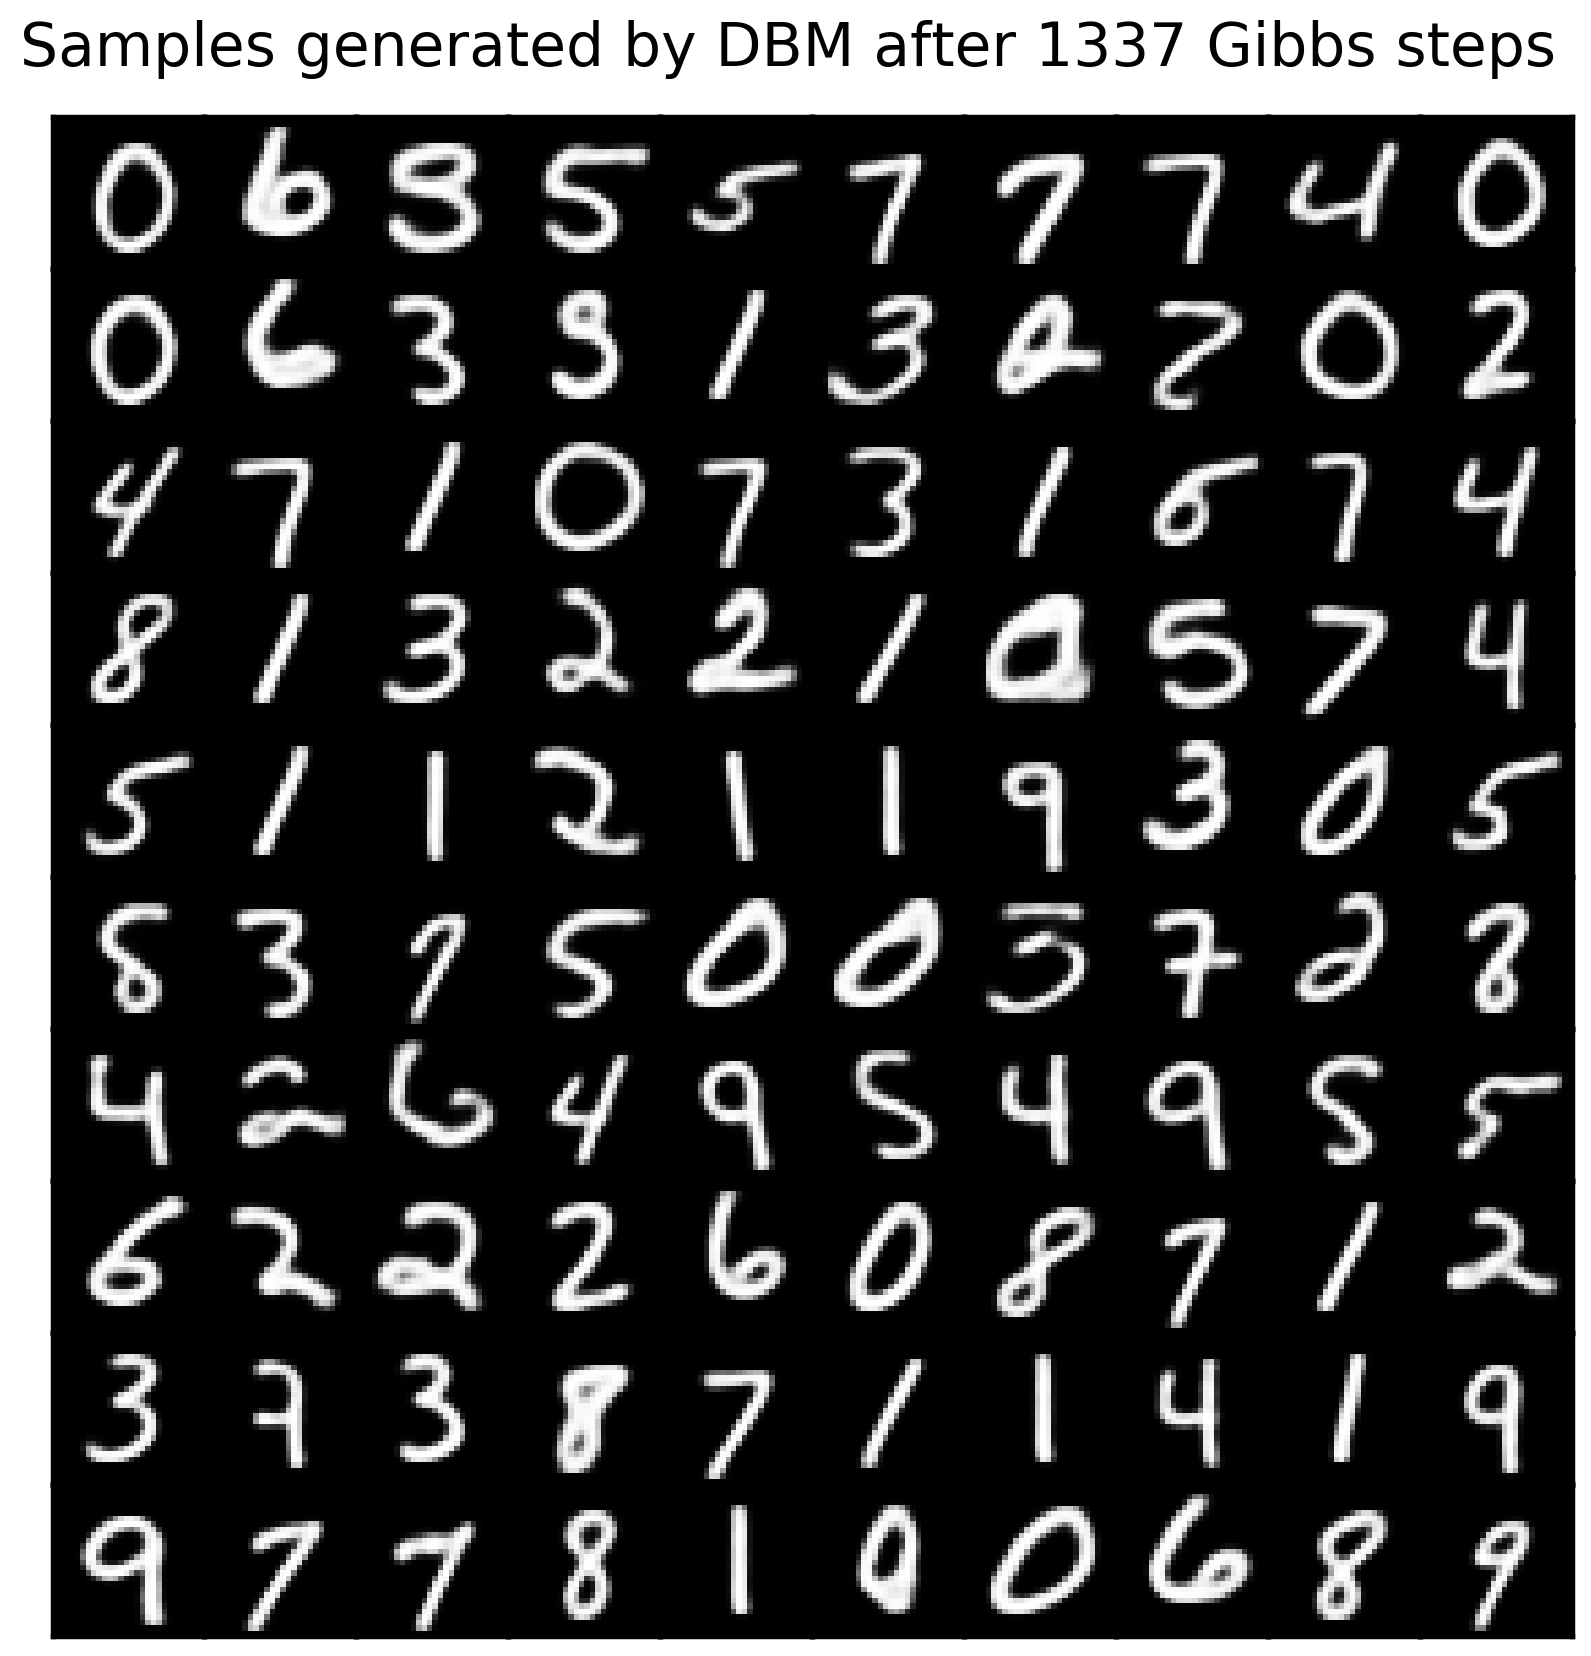
\includegraphics[width=2.8in]{dbm-mnist-latest/samples.png}
\\[2em]
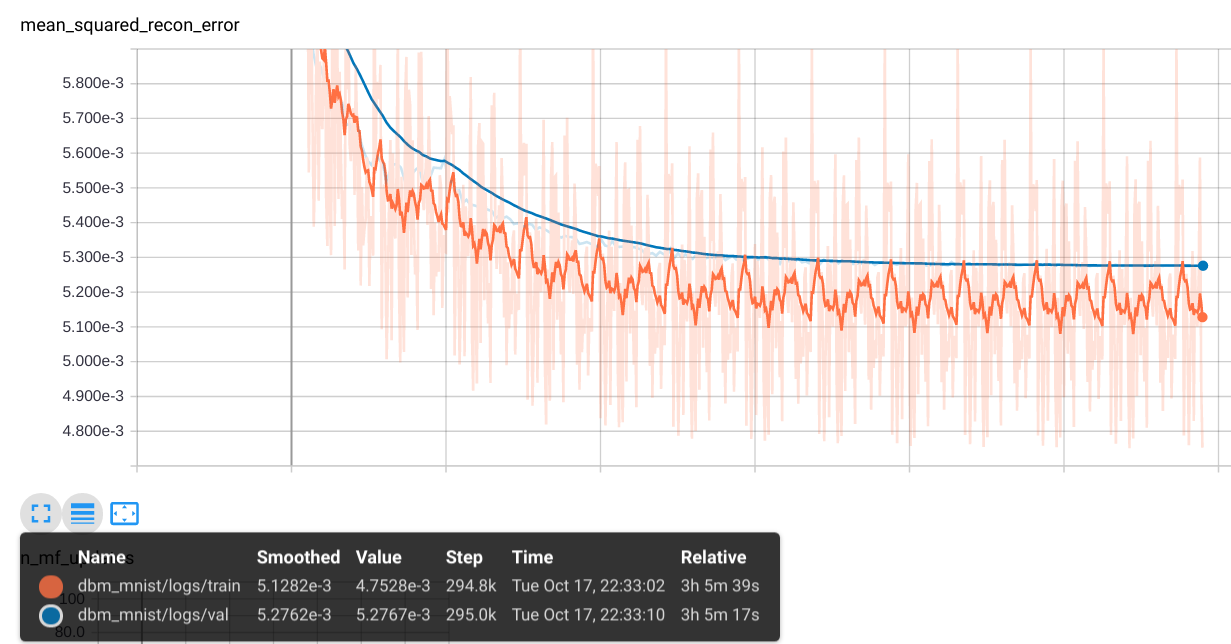
\includegraphics[width=5.6in]{dbm-mnist-latest/msre.png}
\caption{\emph{Top}: random subset of training data and generated samples by DBM. \emph{Bottom}: MSRE of DBM}.
\end{mdframed}
\end{figure}

\clearpage
\newpage
\subsection{Experiments on CIFAR-10}
\subsubsection{Before sparsity targets, AIS; naive training of Gaussian RBM}
\u{Architecture}: 3072-5000-1000 Gaussian-Bernoulli-Multinomial DBM.
\\[0.5em]
\u{Preprocessing}: Zeroing 1000 least significant variance directions as in \cite{krizhevsky2009learning}.
\clearpage

\begin{figure}[h]
\begin{mdframed}
\centering
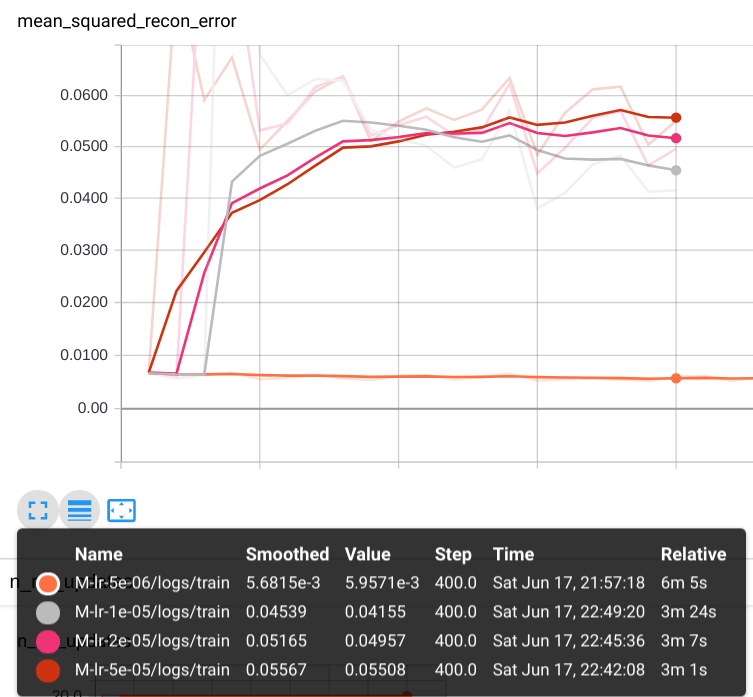
\includegraphics[width=5in]{dbm-cifar/instab.png}
\\[2em]
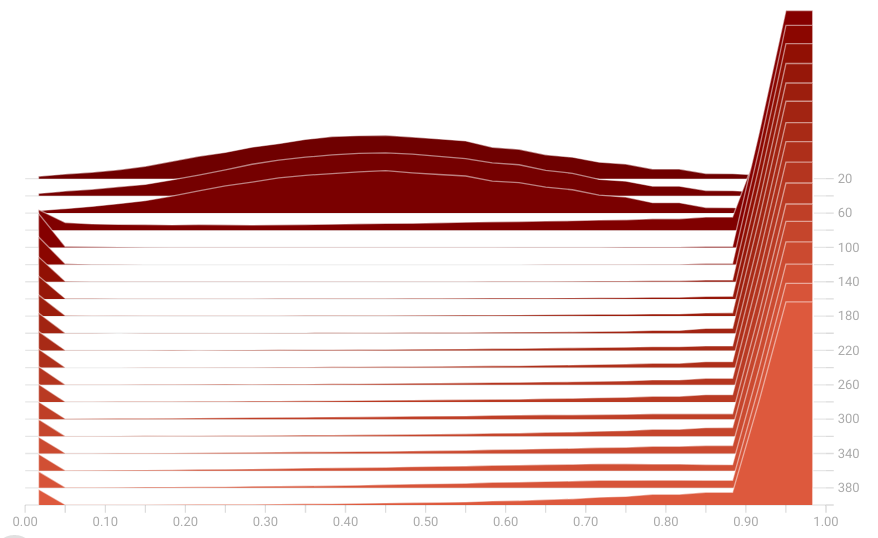
\includegraphics[height=2in]{dbm-cifar/mu_before.png}
\quad
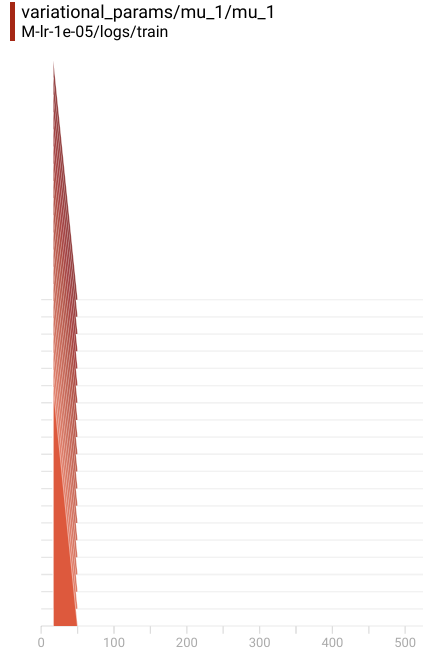
\includegraphics[height=2in]{dbm-cifar/mu_1_before.png}
\caption{After pre-training during the joint training severe instabilities occured unless an extremely small learning rate was used. After inspection of distribution of variational parameters (in first and second hidden layers), \u{the reason became clear}: the total input to first layer hidden units was too large $\Rightarrow$ "overshoot" of sigmoid units. For training 5k random images were used.}
\end{mdframed}
\end{figure}

\clearpage

\begin{figure}[h]
\begin{mdframed}
\centering
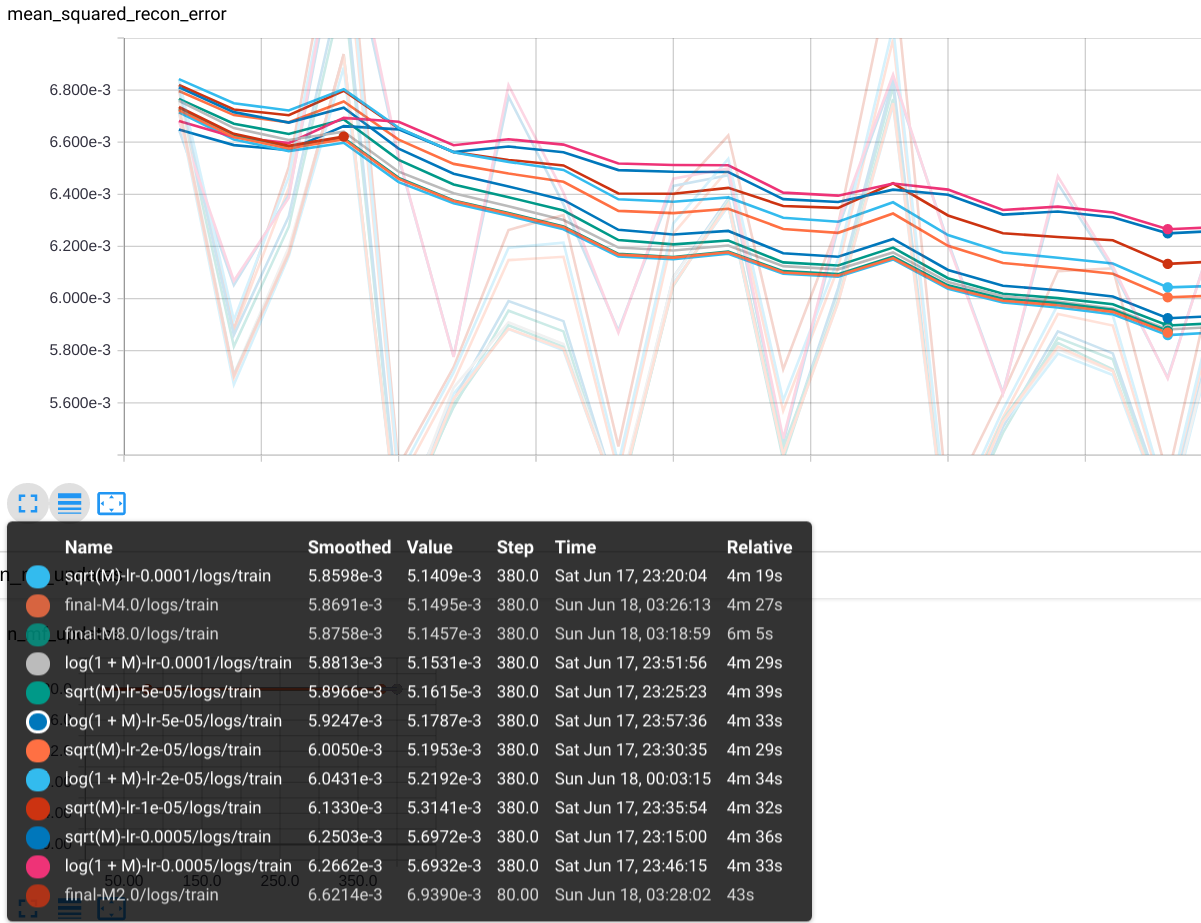
\includegraphics[width=5in]{dbm-cifar/instab_resolved.png}
\\[2em]
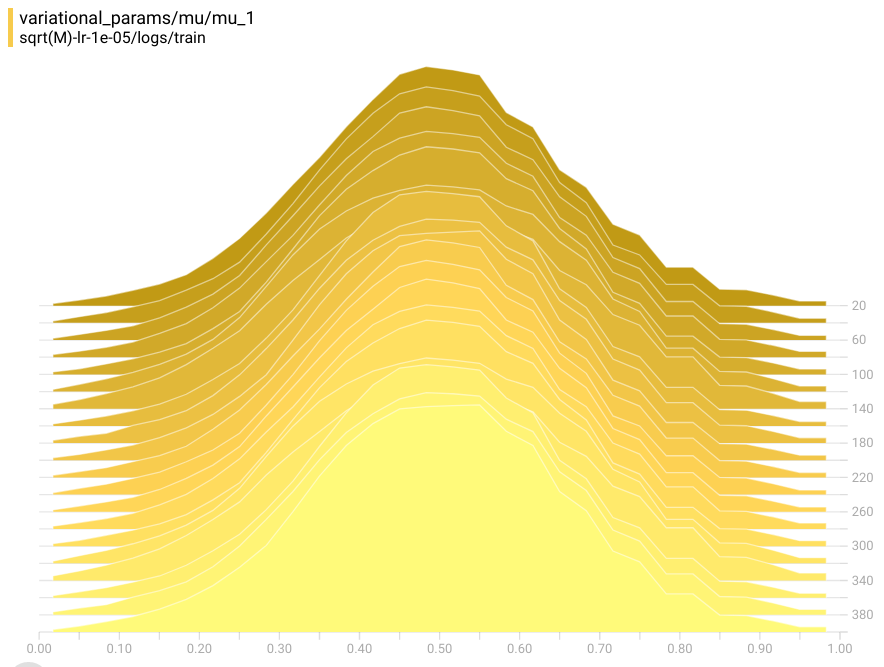
\includegraphics[height=2in]{dbm-cifar/mu_after.png}
\quad
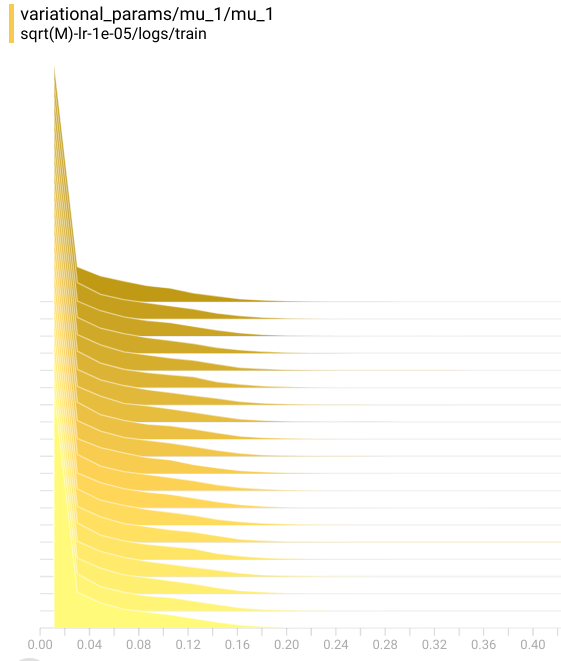
\includegraphics[height=2in]{dbm-cifar/mu_1_after.png}
\caption{\emph{Top}: reconstruction error when the total input from Multinomial layer were multiplied by $\frac{1}{\sqrt{M}}$ and $\frac{\log(1+M)}{M}$ from previous experiment. \emph{Bottom}: distribution of variational parameters in first and second hidden layers after $\frac{1}{\sqrt{M}}$ scaling were applied.}
\end{mdframed}
\end{figure}

\clearpage

\begin{figure}[h]
\begin{mdframed}
\centering
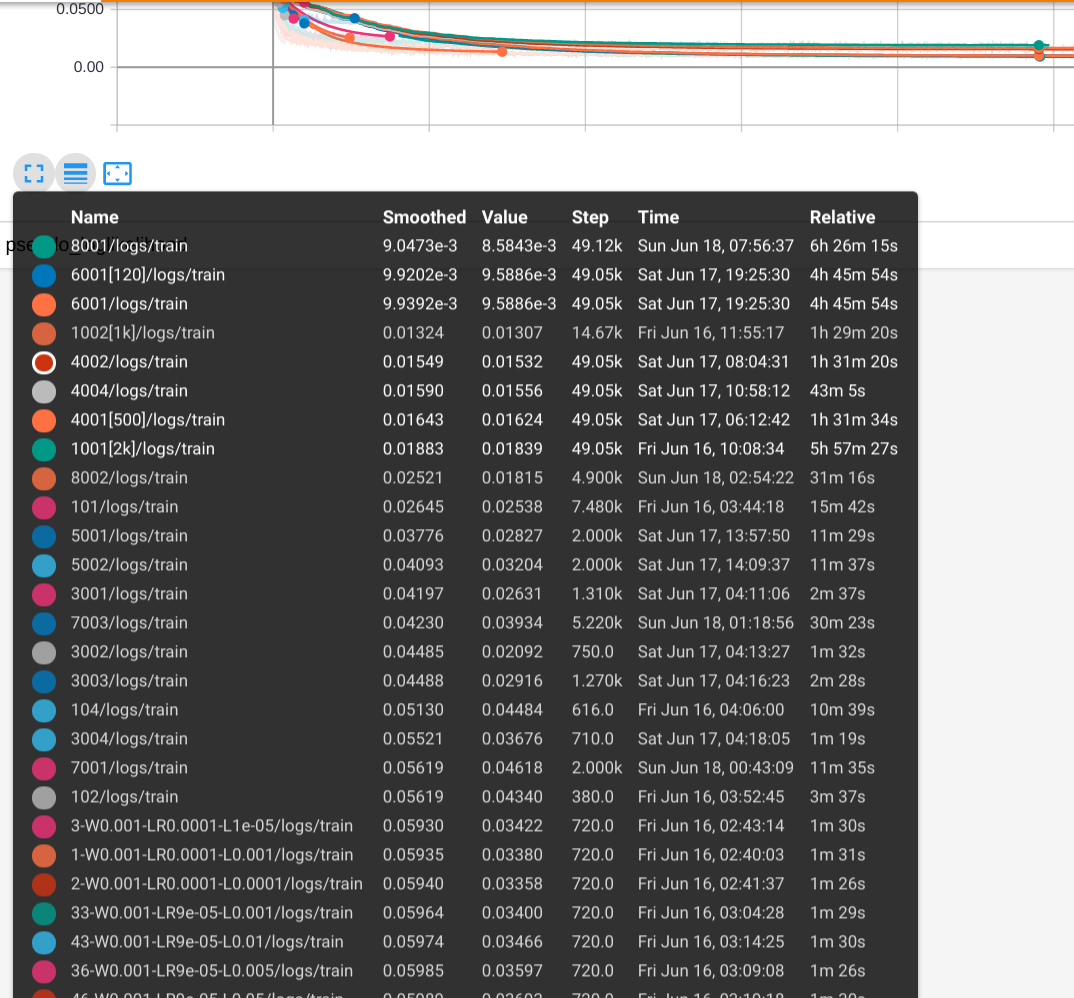
\includegraphics[width=6in]{dbm-cifar/mrbm.png}
\caption{Reconstruction error of Multinomial RBM trained on extracted features $\mb{q}_i=p(\mb{h}|\mb{v}=\mb{x}_i; \bs{\psi})$ of Gaussian RBM on full dataset.}
\end{mdframed}
\end{figure}

\clearpage

\begin{figure}[h]
\begin{mdframed}
\centering
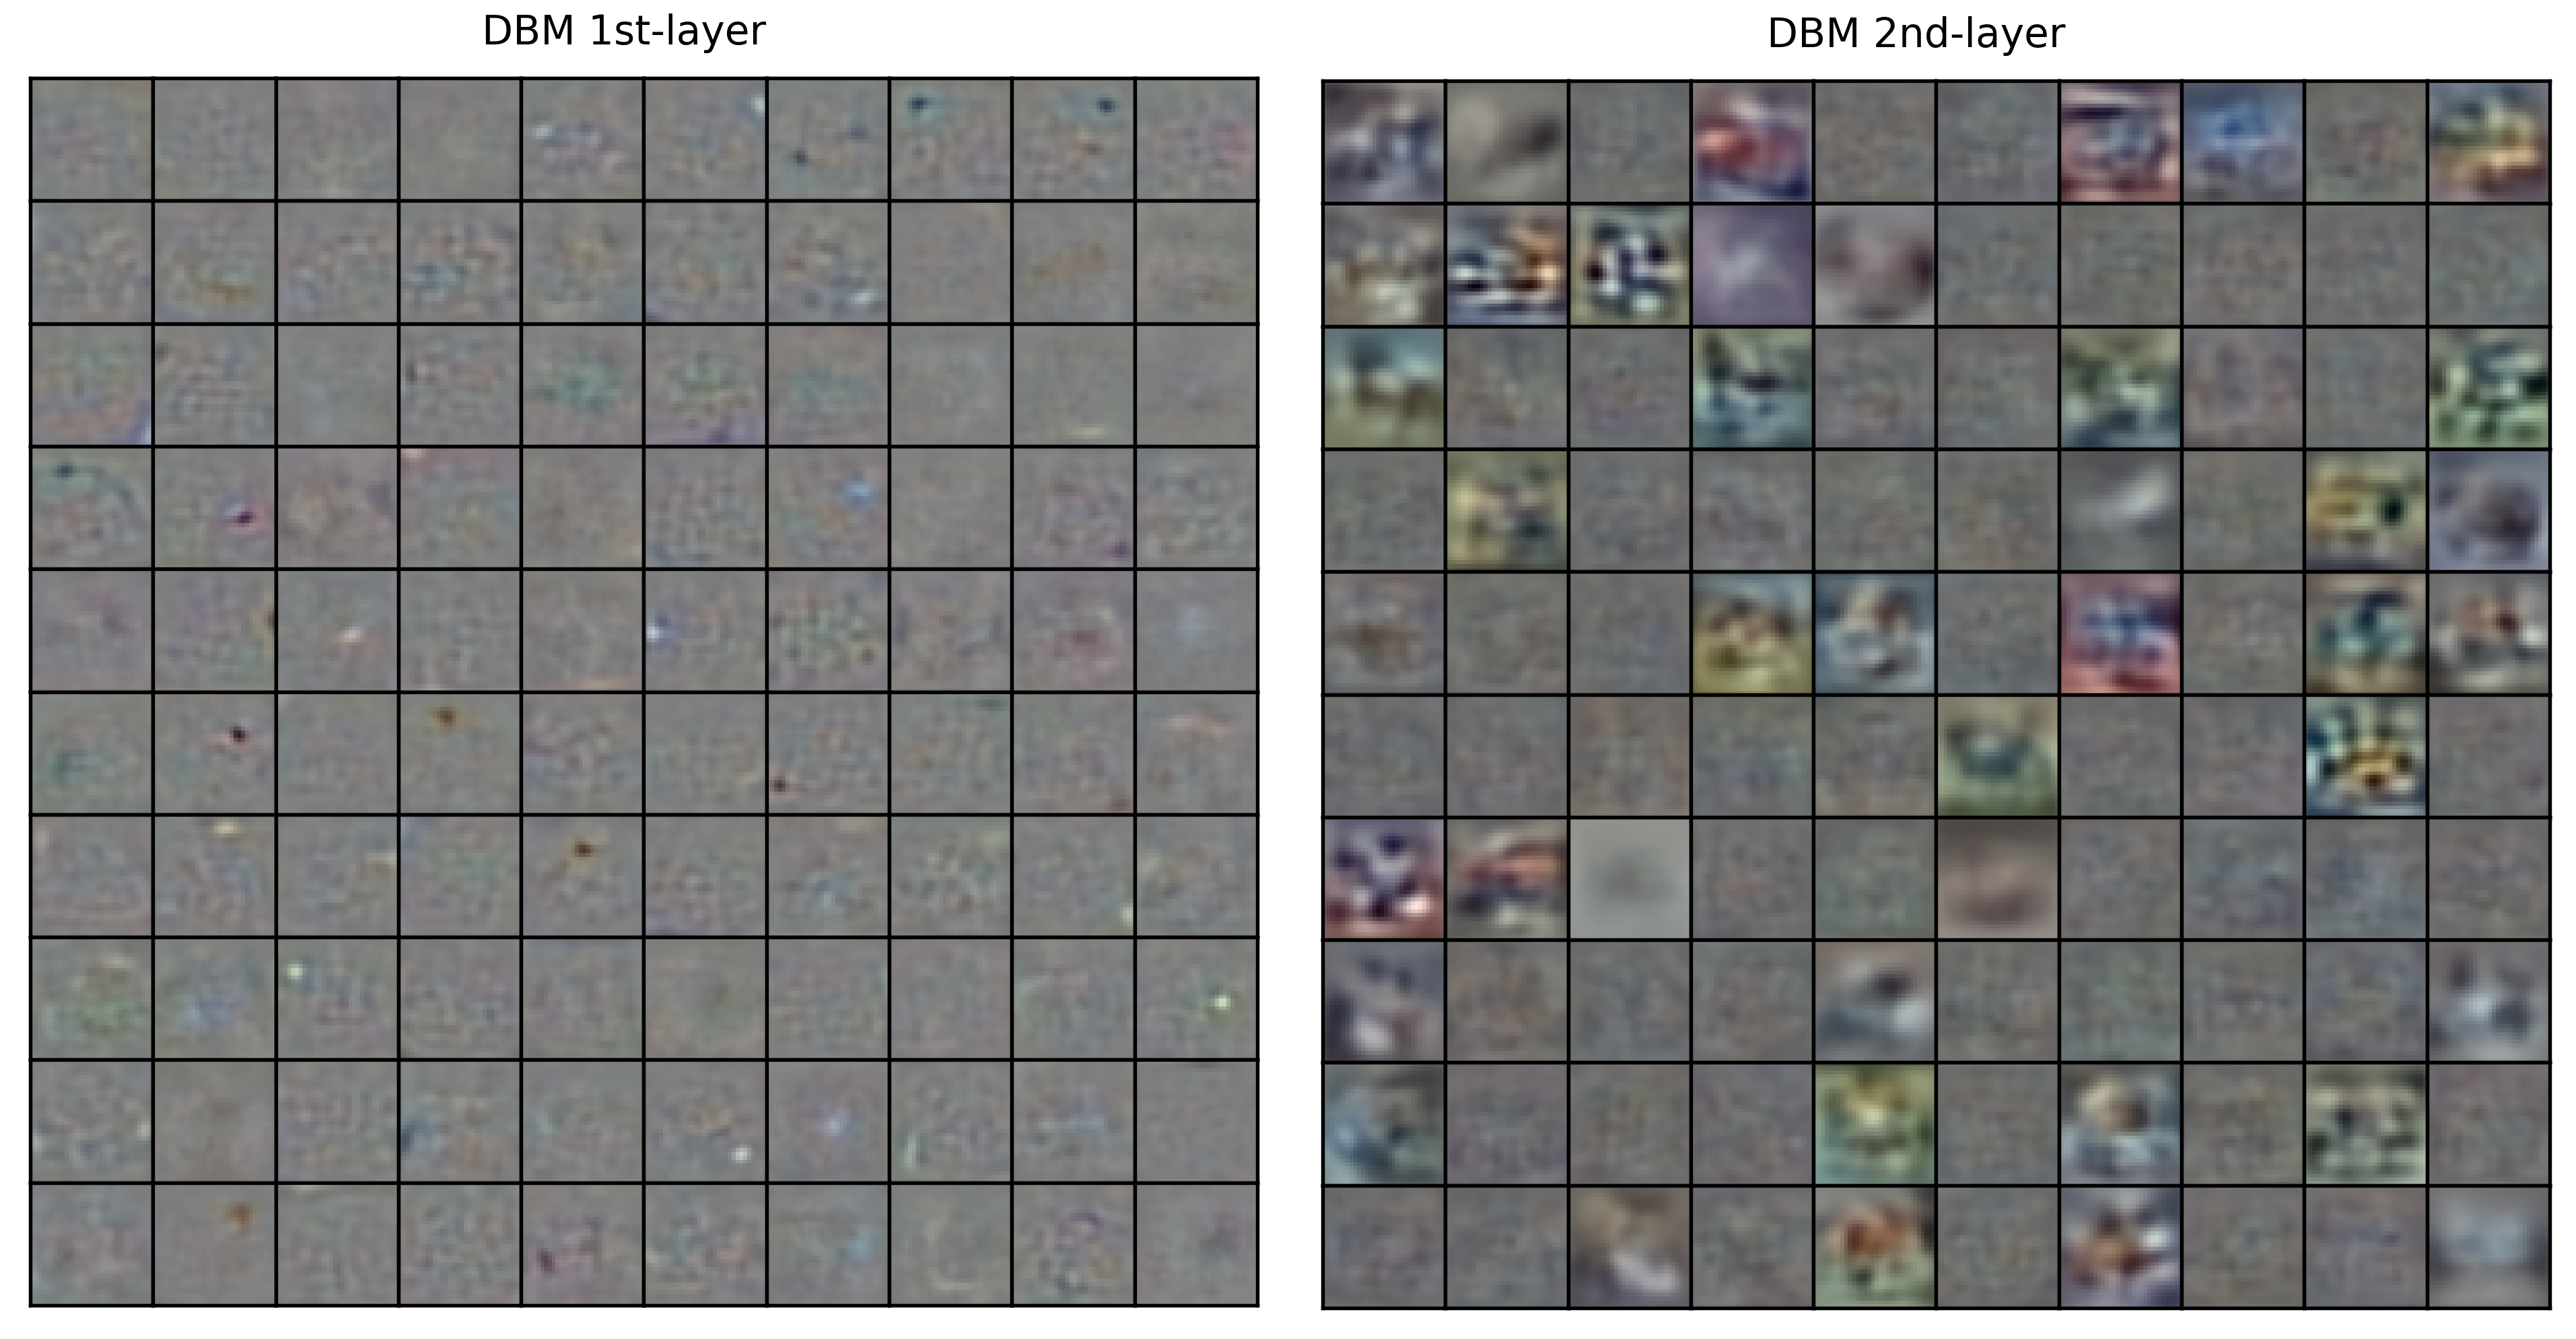
\includegraphics[width=5.2in]{dbm-cifar/filters.png}
\\[2em]
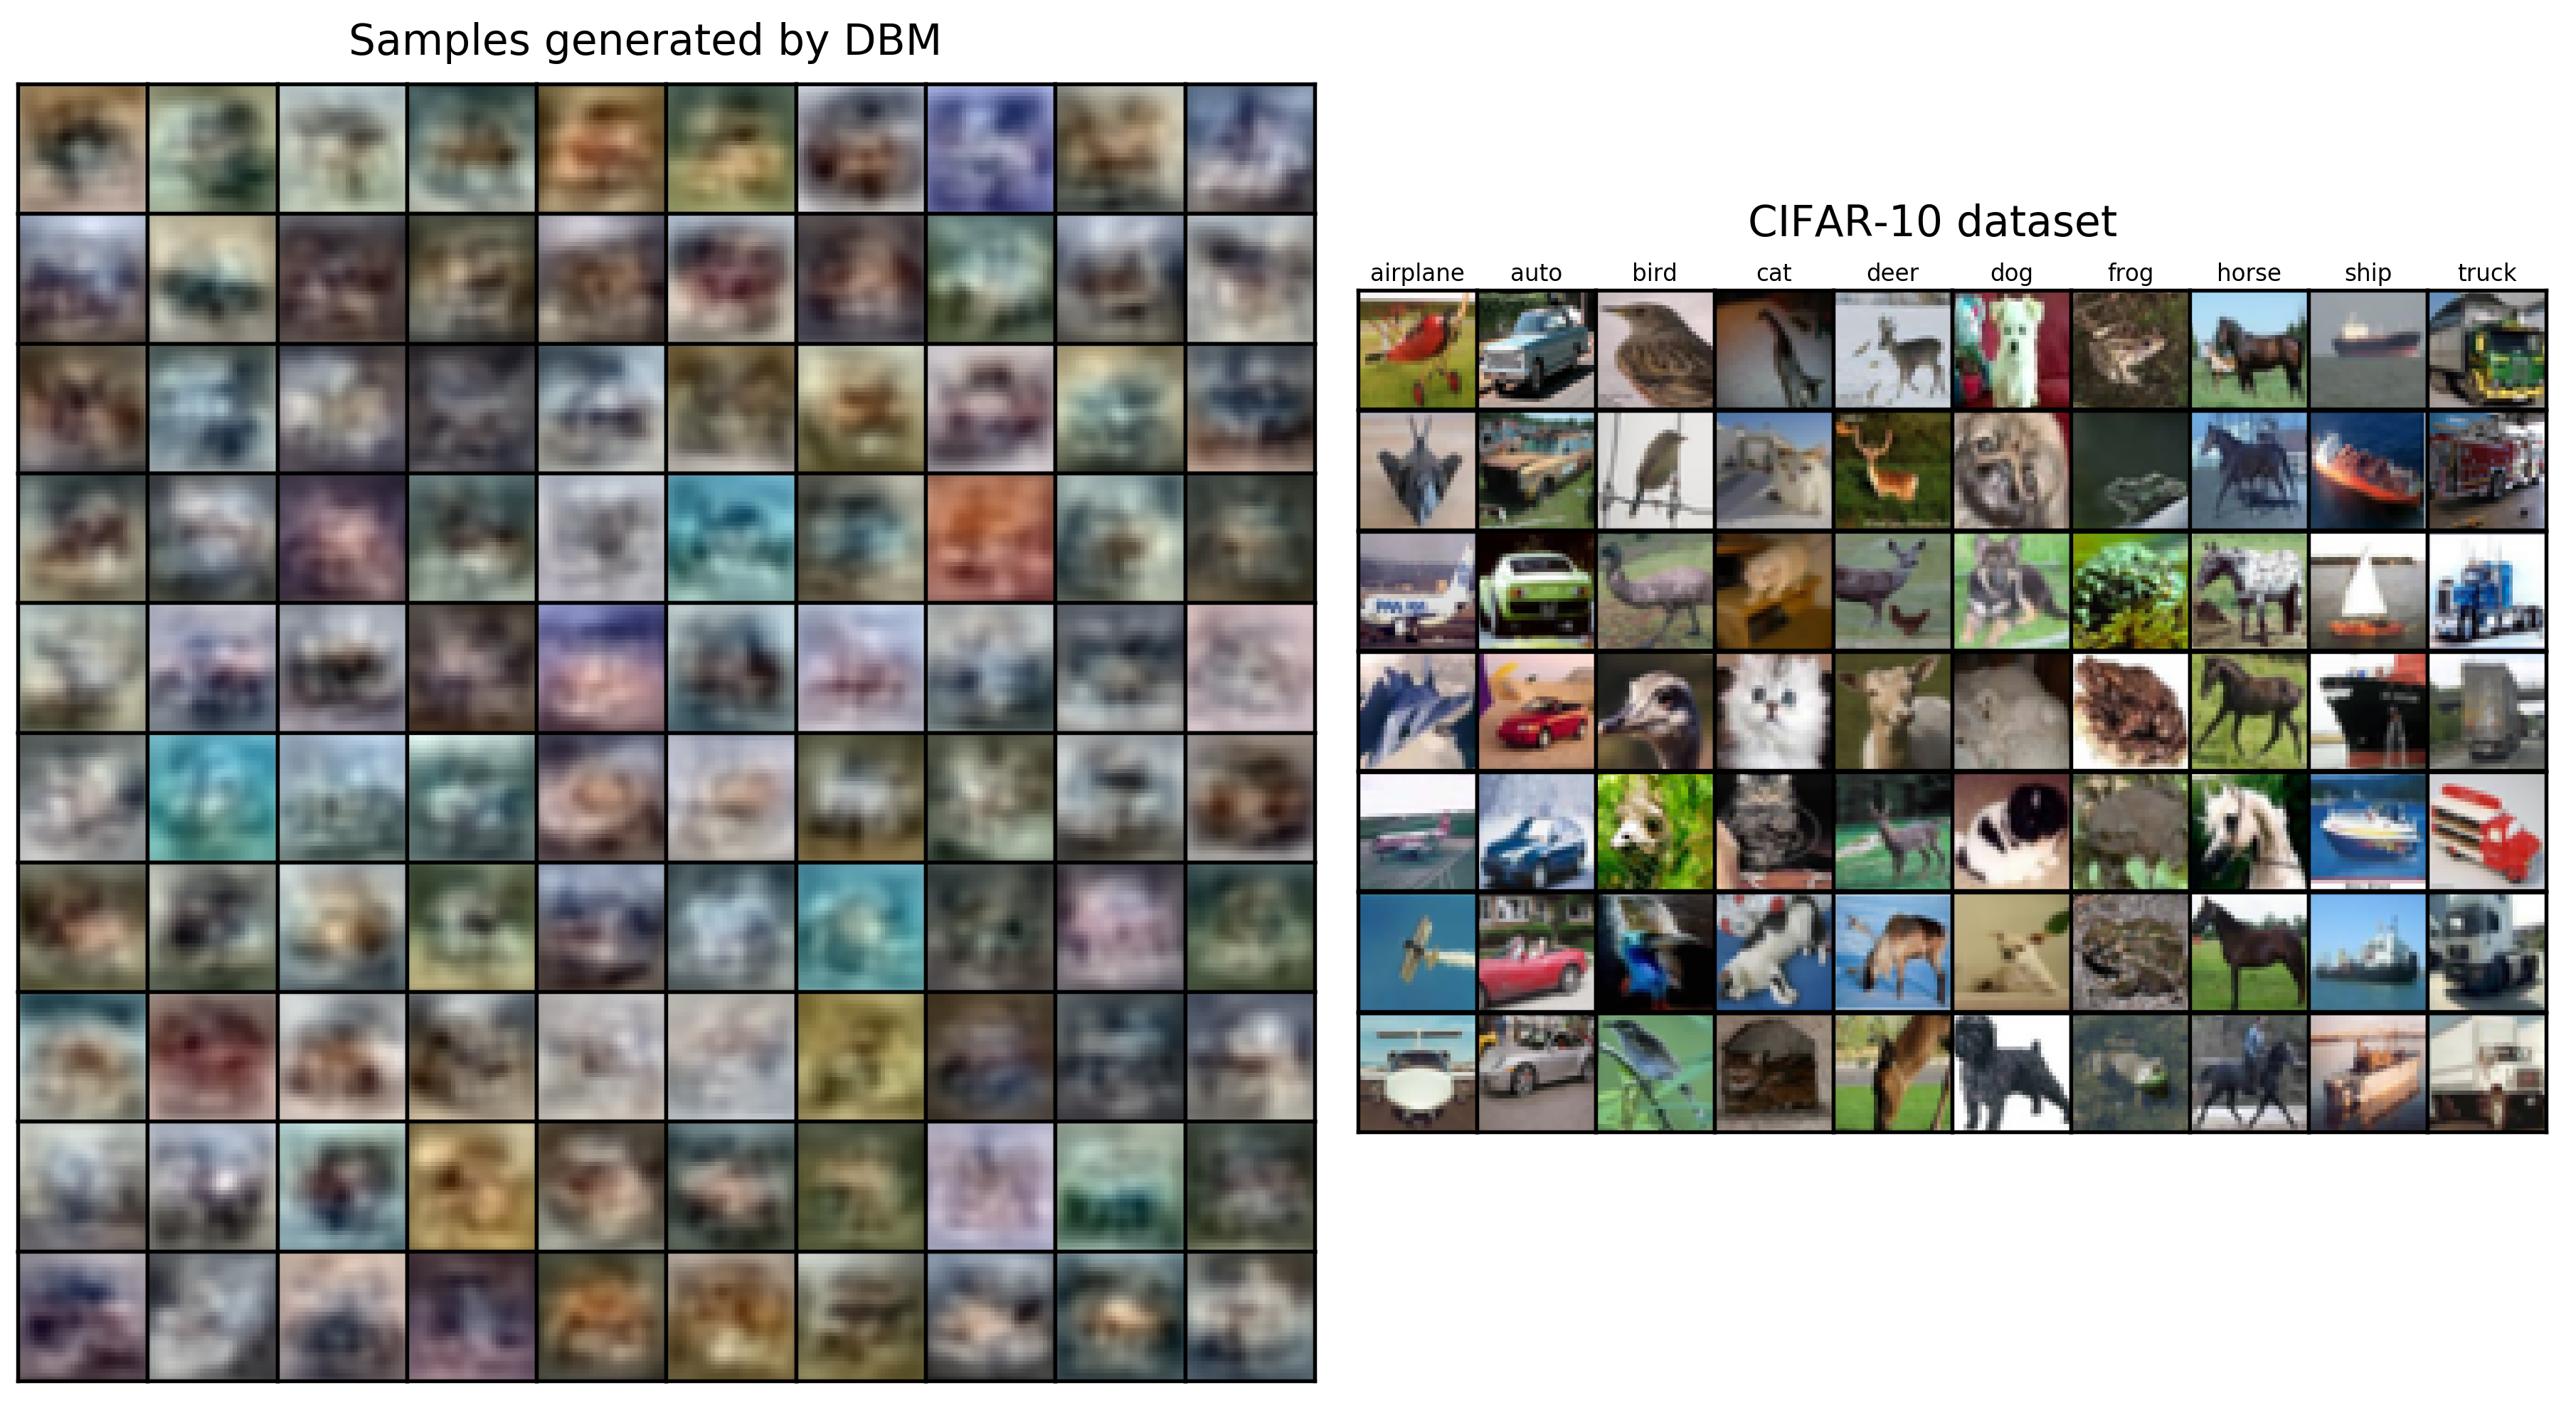
\includegraphics[width=5.2in]{dbm-cifar/samples.png}
\caption{Best model trained on full CIFAR-10 dataset in this phase. 2nd layer filters are visualized using method of \emph{weighted linear combinations} \cite{erhan2009visualizing}. \tb{\emph{G-RBM Hyperparams}}: L2 0.001, batch size 100, 99 epochs, lr 0.0005, momentum $0.5\rightarrow 0.9$, 1 Gibbs step, w\_std 0.0008, biases to 0, $\bs{\sigma}$ from data; sample both visible and hidden states. \tb{\emph{M-RBM Hyperparams}}: L2 0.05, batch size 100, 118 epochs, learning rate 0.0001, momentum $0.5\rightarrow 0.9$, 1 Gibbs step, number of samples $M=K=1000$, w\_std 0.01, biases to zero; sample only hidden states (for visible use probabilities w/o sampling); no scaling of total input. \tb{\emph{DBM Hyperparams}}: 100 particles, initialize from data for all layers, 1 Gibbs step, 25 mean-field updates ($10^{-13}$ tolerance), momentum $0.5\rightarrow 0.9$, learning rate $9\cdot10^{-5}\rightarrow 10^{-5}$ by dividing by $(1.000015)^{600}$ each epoch, 200 epochs, batch size 50, L2 $=0$, max norm $=2$; sample all visible and hidden states.}
\end{mdframed}
\end{figure}

\clearpage
\newpage
\subsubsection{"naive" training of Gaussian RBM}
\begin{figure}[h]
\begin{mdframed}
\centering
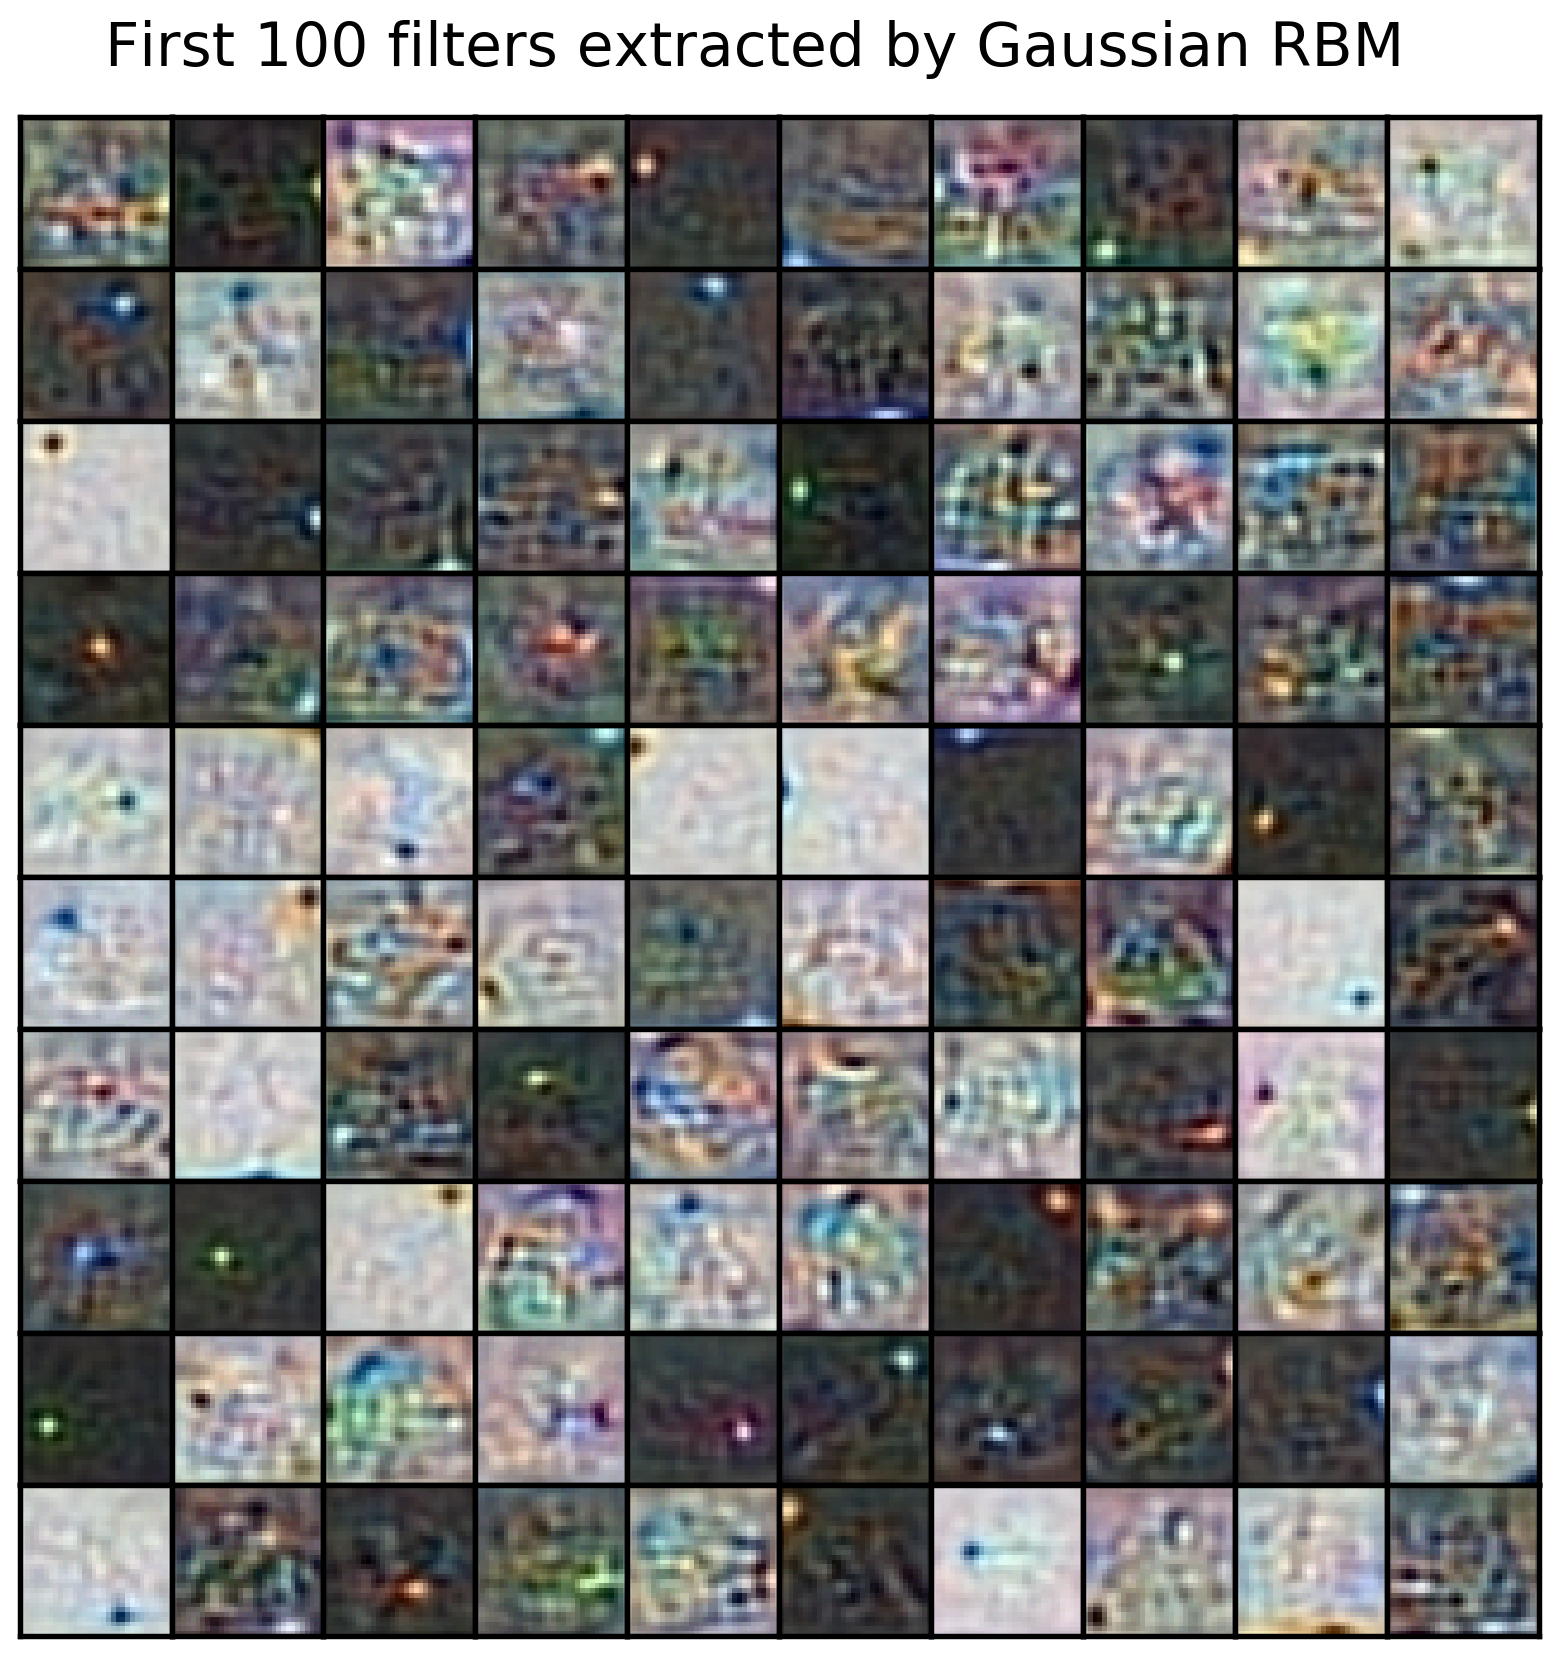
\includegraphics[width=2.5in]{dbm-cifar-naive/grbm.png}
\quad
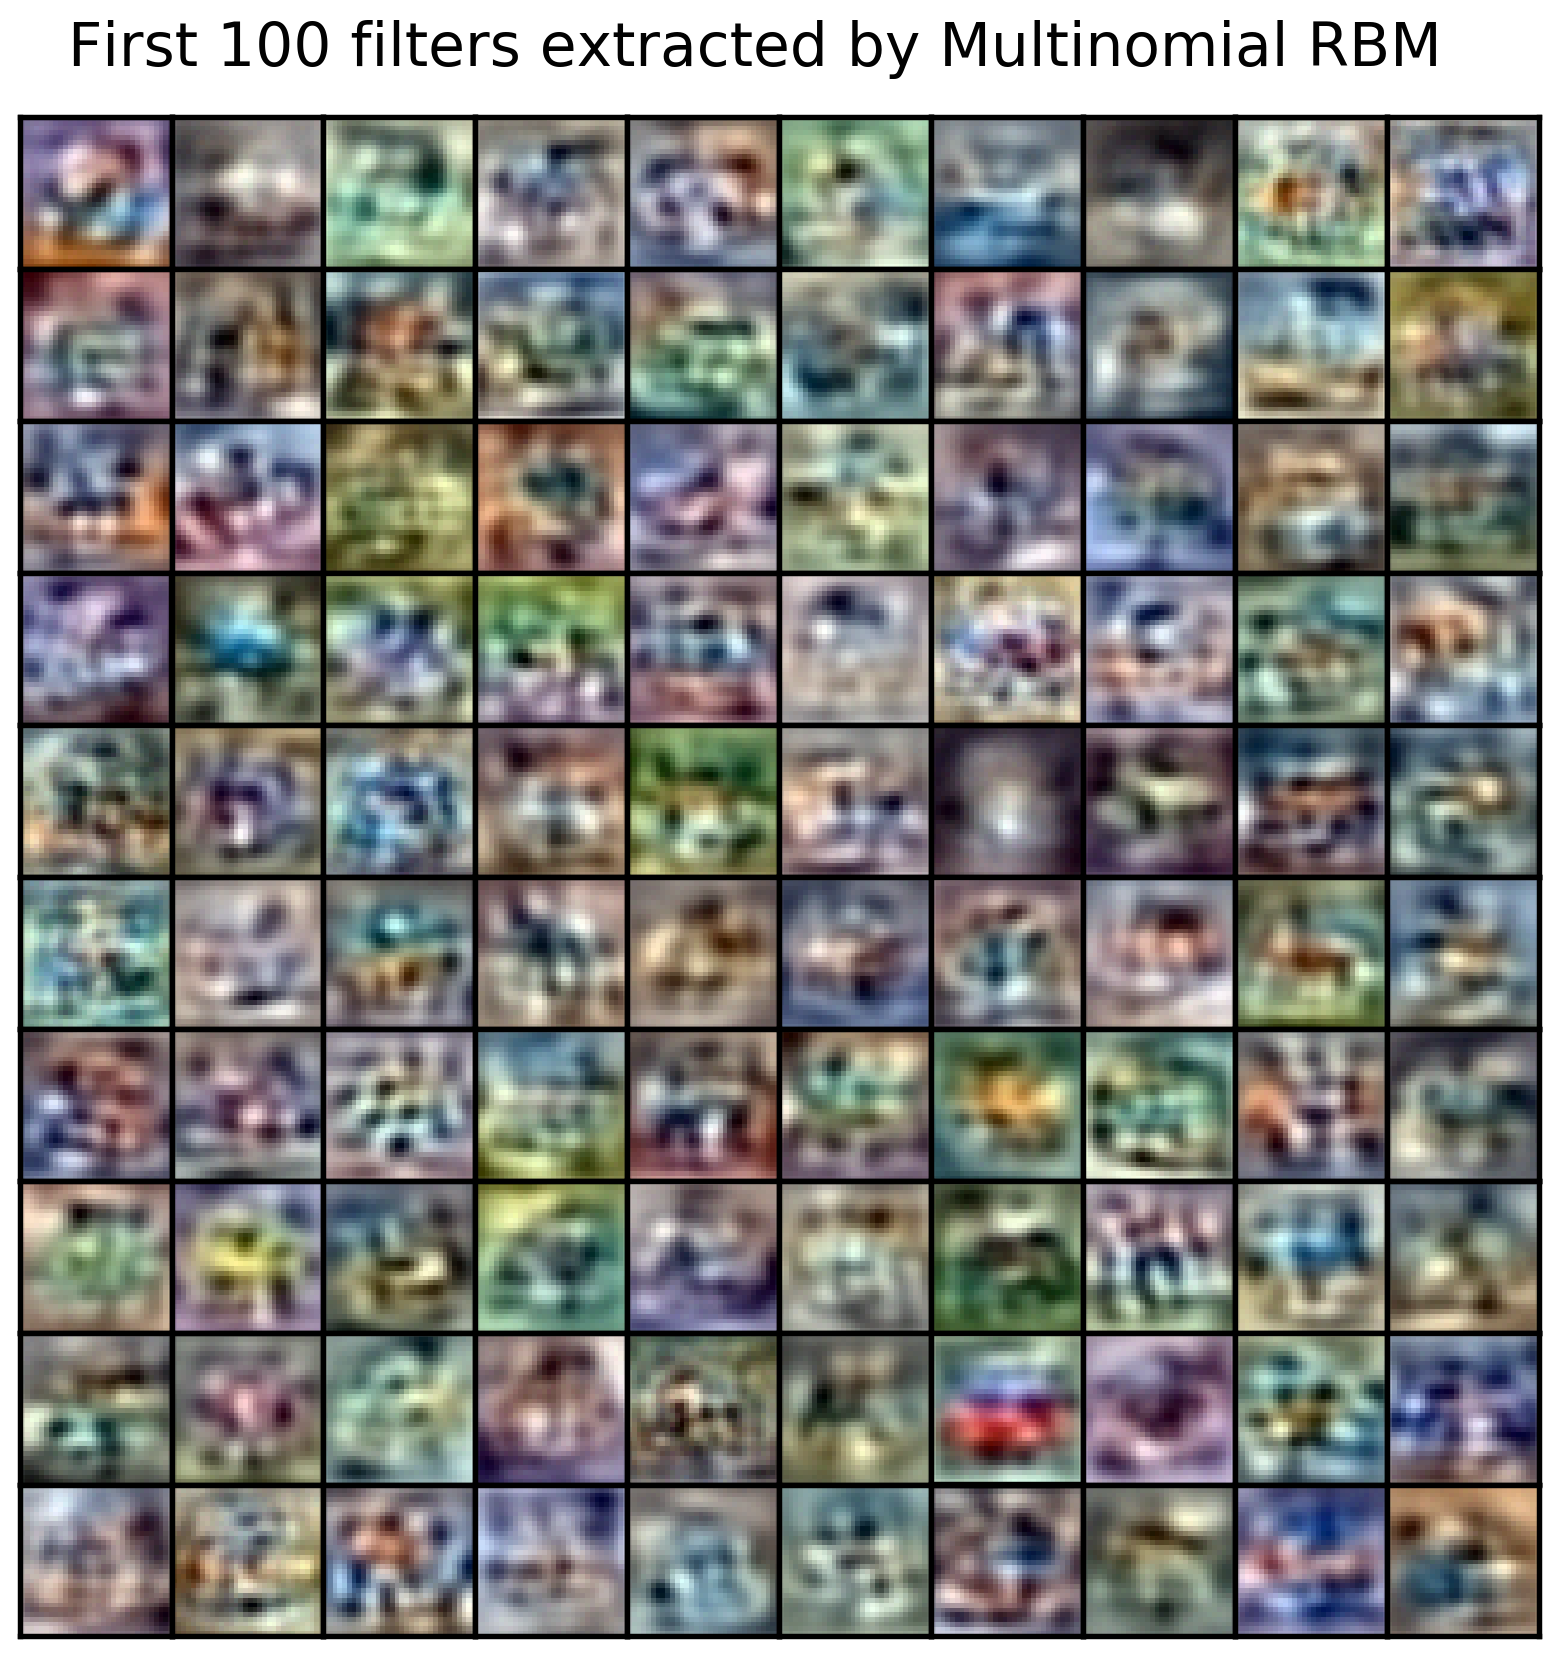
\includegraphics[width=2.5in]{dbm-cifar-naive/mrbm.png}
\\[2em]
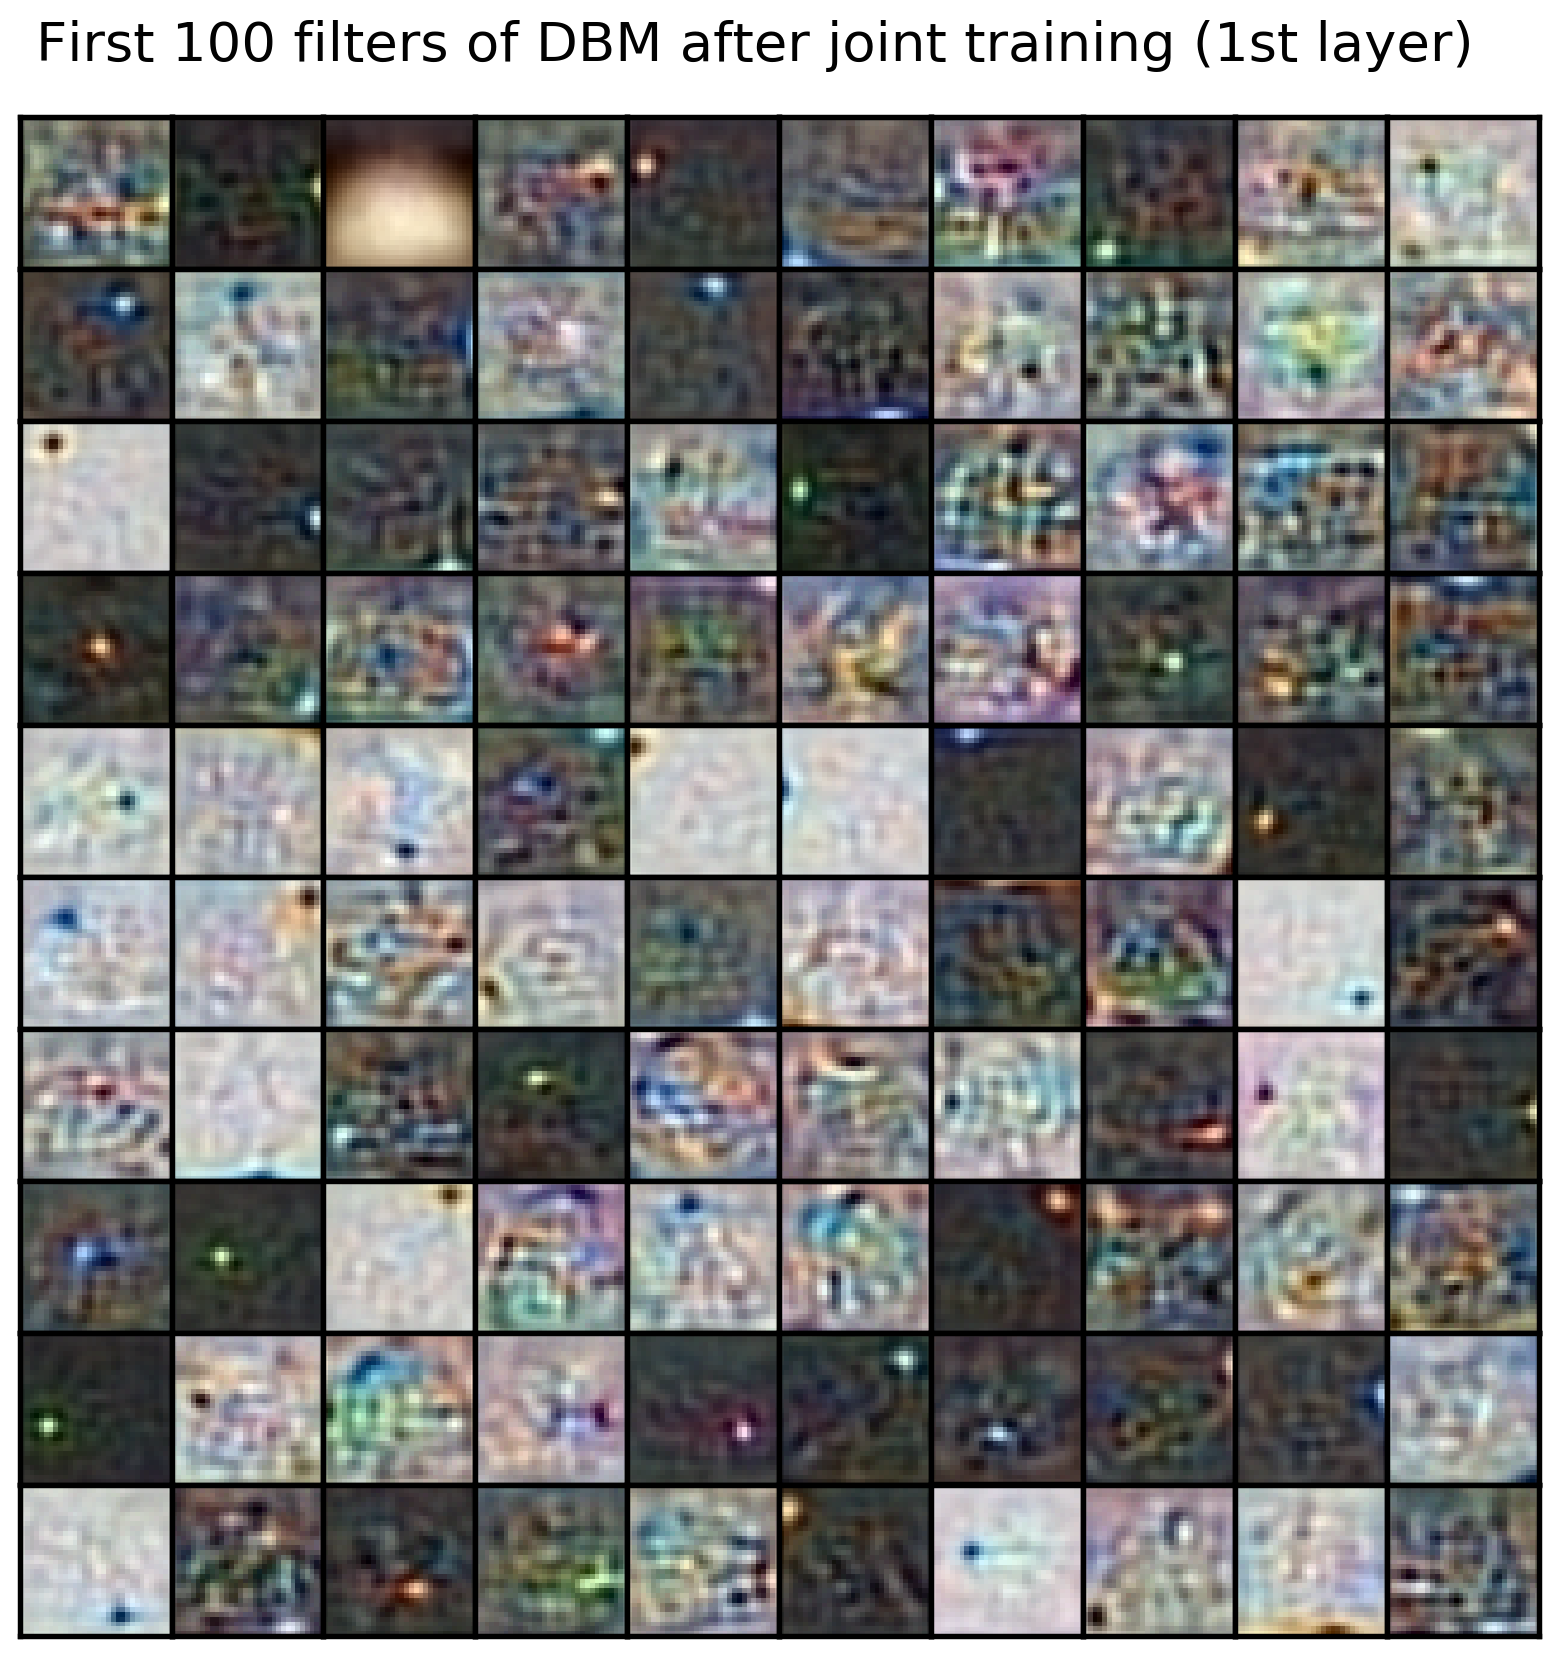
\includegraphics[width=2.5in]{dbm-cifar-naive/W1_joint.png}
\quad
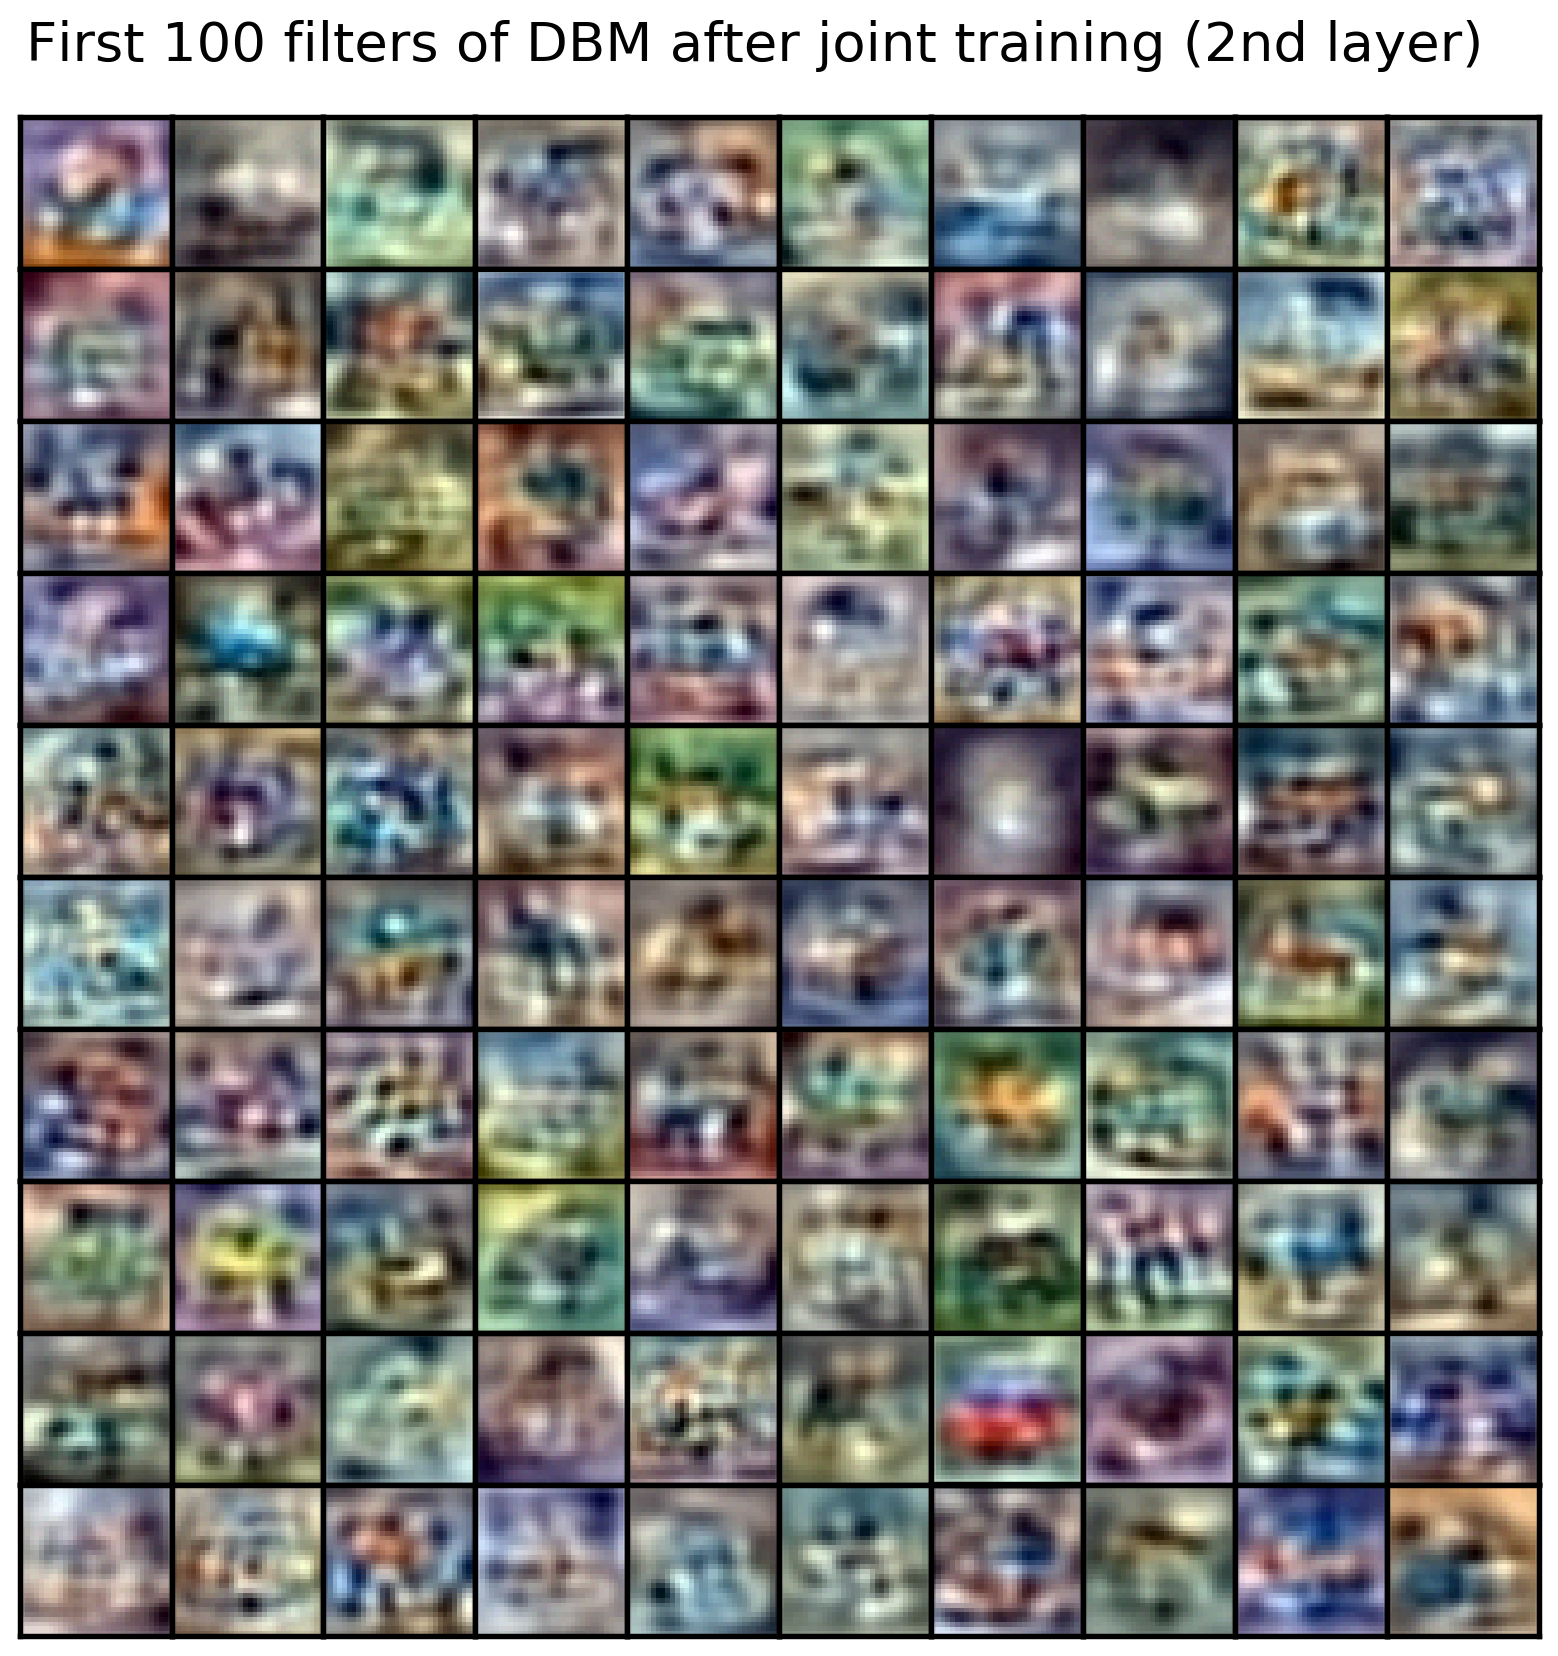
\includegraphics[width=2.5in]{dbm-cifar-naive/W2_joint.png}
\caption{Weight filters}.
\end{mdframed}
\end{figure}

\clearpage
\subsubsection{"naive" training of Gaussian RBM}
\begin{figure}[h]
\begin{mdframed}
\centering
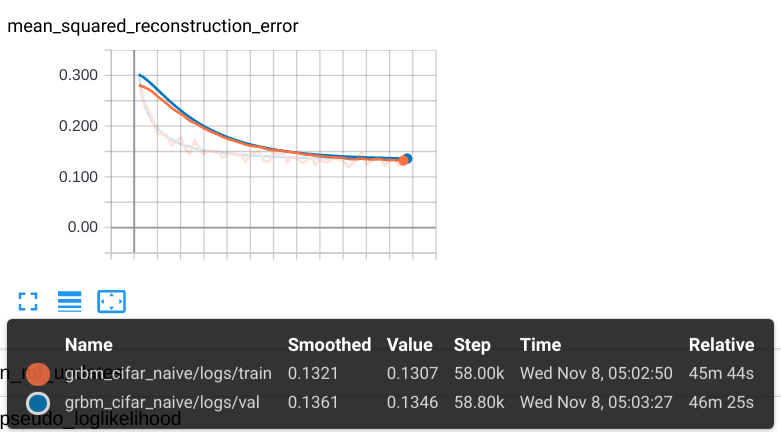
\includegraphics[width=3.5in]{dbm-cifar-naive/grbm_msre.png}
\quad
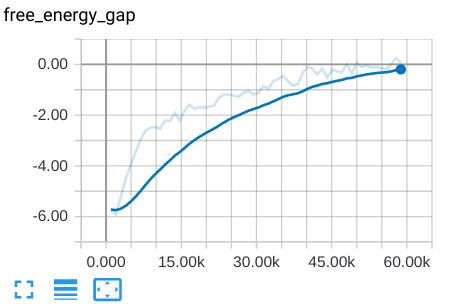
\includegraphics[width=2.4in]{dbm-cifar-naive/grbm_feg.png}
\\[4em]
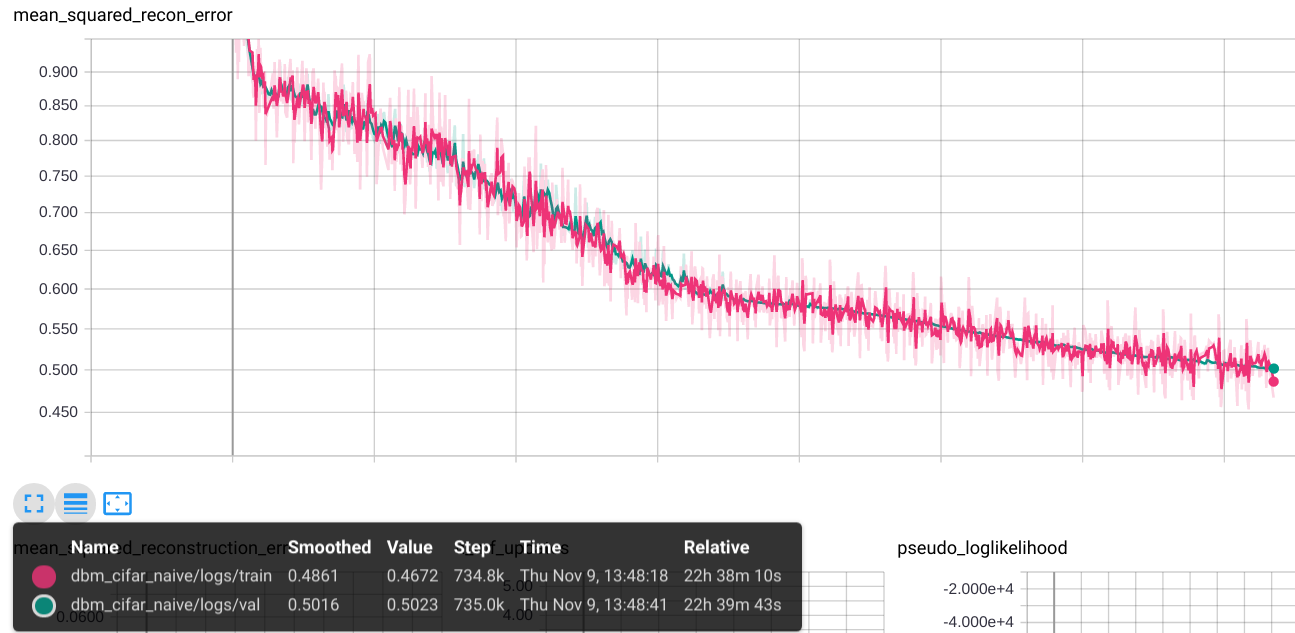
\includegraphics[width=5.4in]{dbm-cifar-naive/dbm_msre.png}
\caption{\emph{Top}: reconstruction error and free nergy gap of Gaussian RBM. \emph{Bottom}: reconstruction error of DBM after joint training.}.
\end{mdframed}
\end{figure}

\clearpage
\newpage
\subsubsection{advanced training of Gaussian RBM}
In this experiment DBM was pretrained and trained on augmented (10 times) CIFAR-10 dataset with shifts by 1 pixel in all directions and mirroring. Also, Gaussian RBM was initialized from 26 small RBMs trained on patches of images, as in \cite{krizhevsky2009learning}, see Fig. \ref{fig:small_rbms}.
\\
\tb{Observation}: in \cite{krizhevsky2009learning} when they initialize large weight matrix, they leave zeros in places where there were no connections in small RBMs during pre-training. I found that using instead random values with small standard deviation (around $10^{-5}$) yield slightly better performance with filters of large RBM smoothed in the neighborhood of corresponding filter from small RBM.
\begin{figure}[h]
\begin{mdframed}
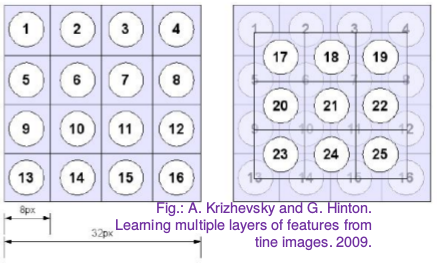
\includegraphics[scale=0.75]{img/small_rbms.png}
\centering
\caption{Pre-training 26 RBMs on patches of images. 26-th RBM was trained on subsampled versions of images.}
\label{fig:small_rbms}
\end{mdframed}
\end{figure}

\clearpage
\begin{figure}[h]
\begin{mdframed}
\centering
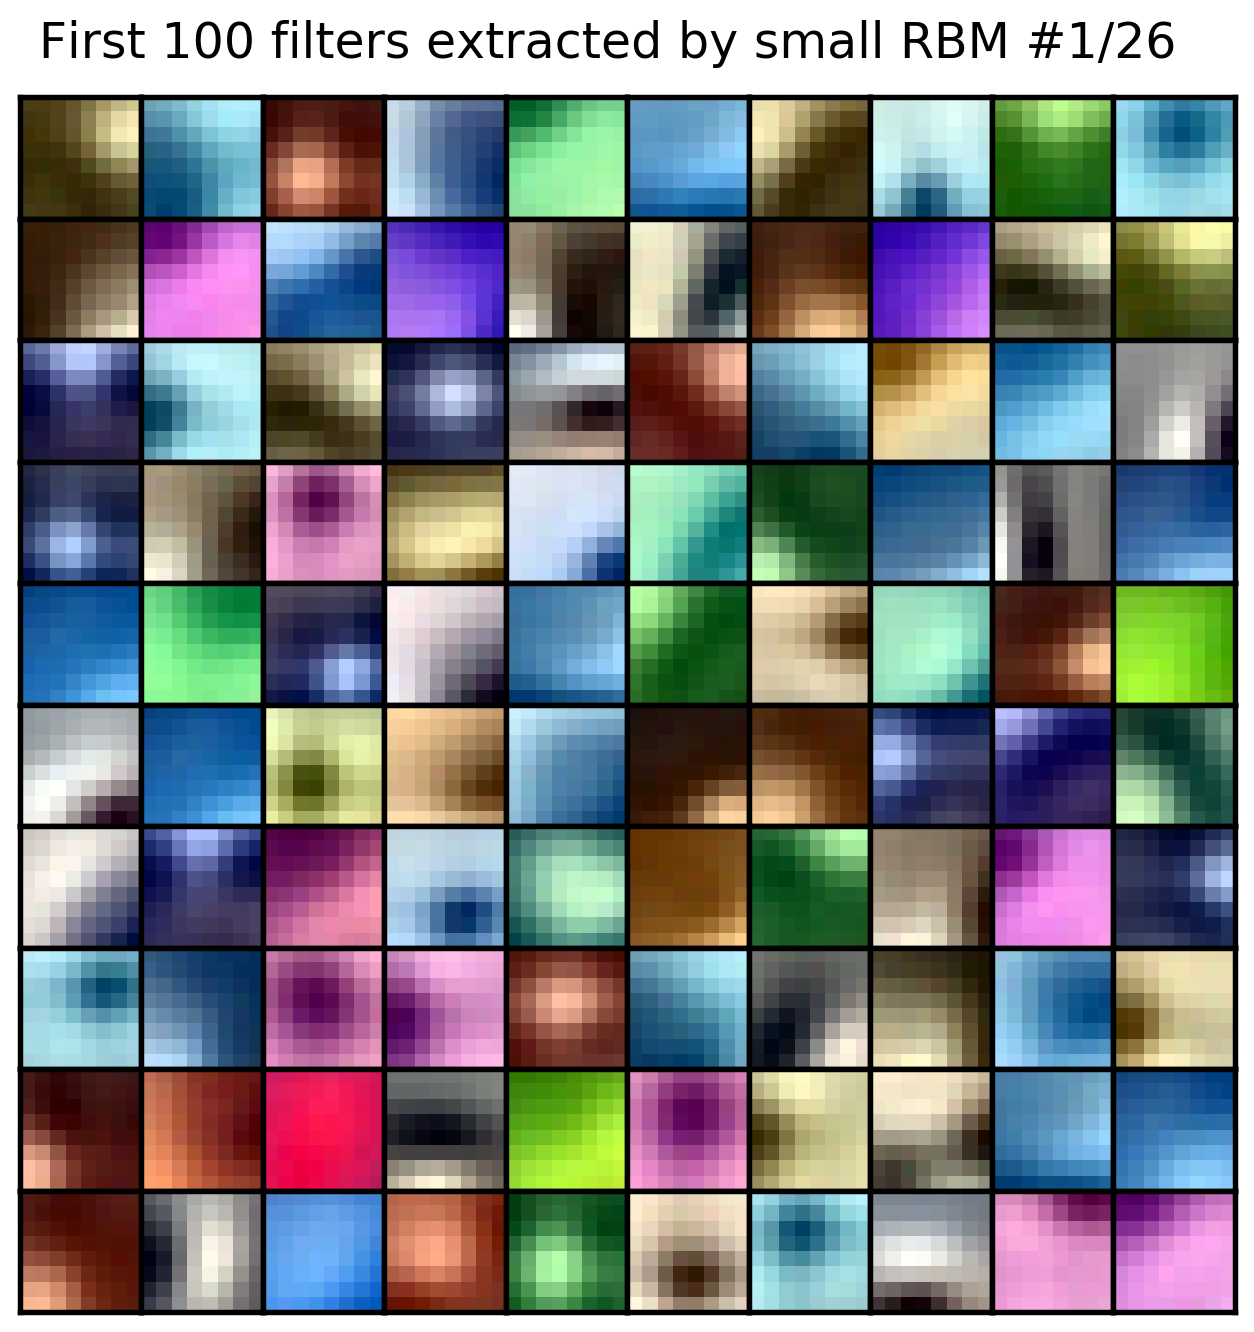
\includegraphics[width=1.6in]{dbm-cifar-latest/rbm_small_0.png}
\quad
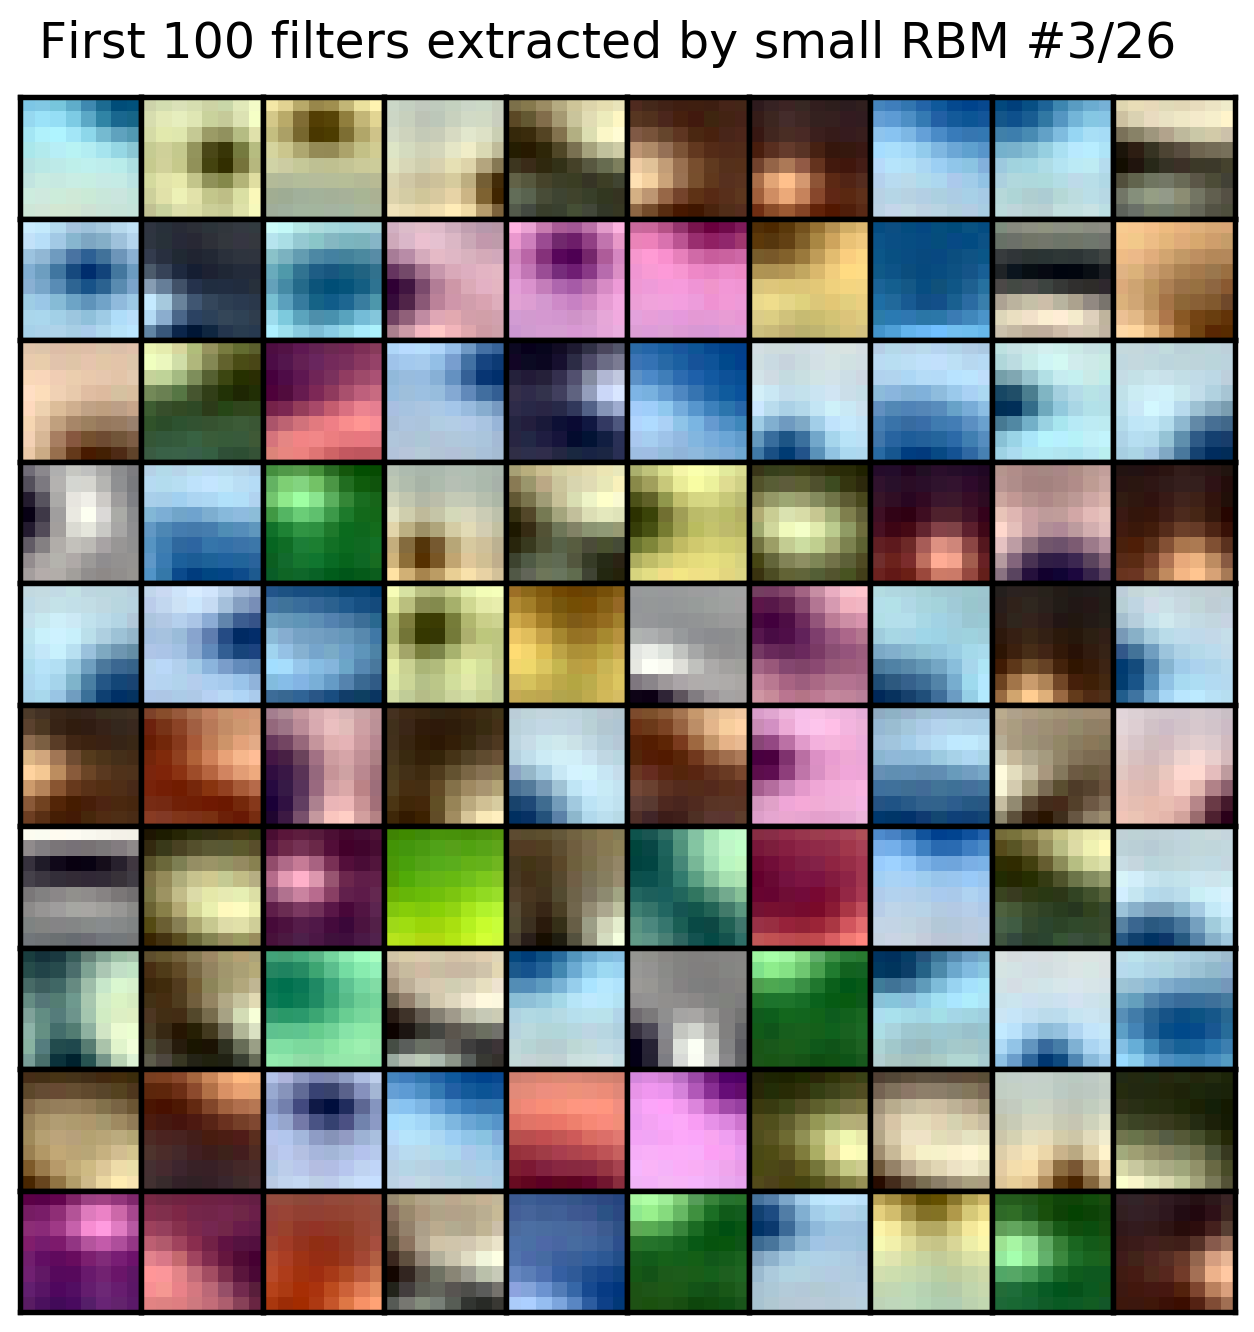
\includegraphics[width=1.6in]{dbm-cifar-latest/rbm_small_2.png}
\\[1em]
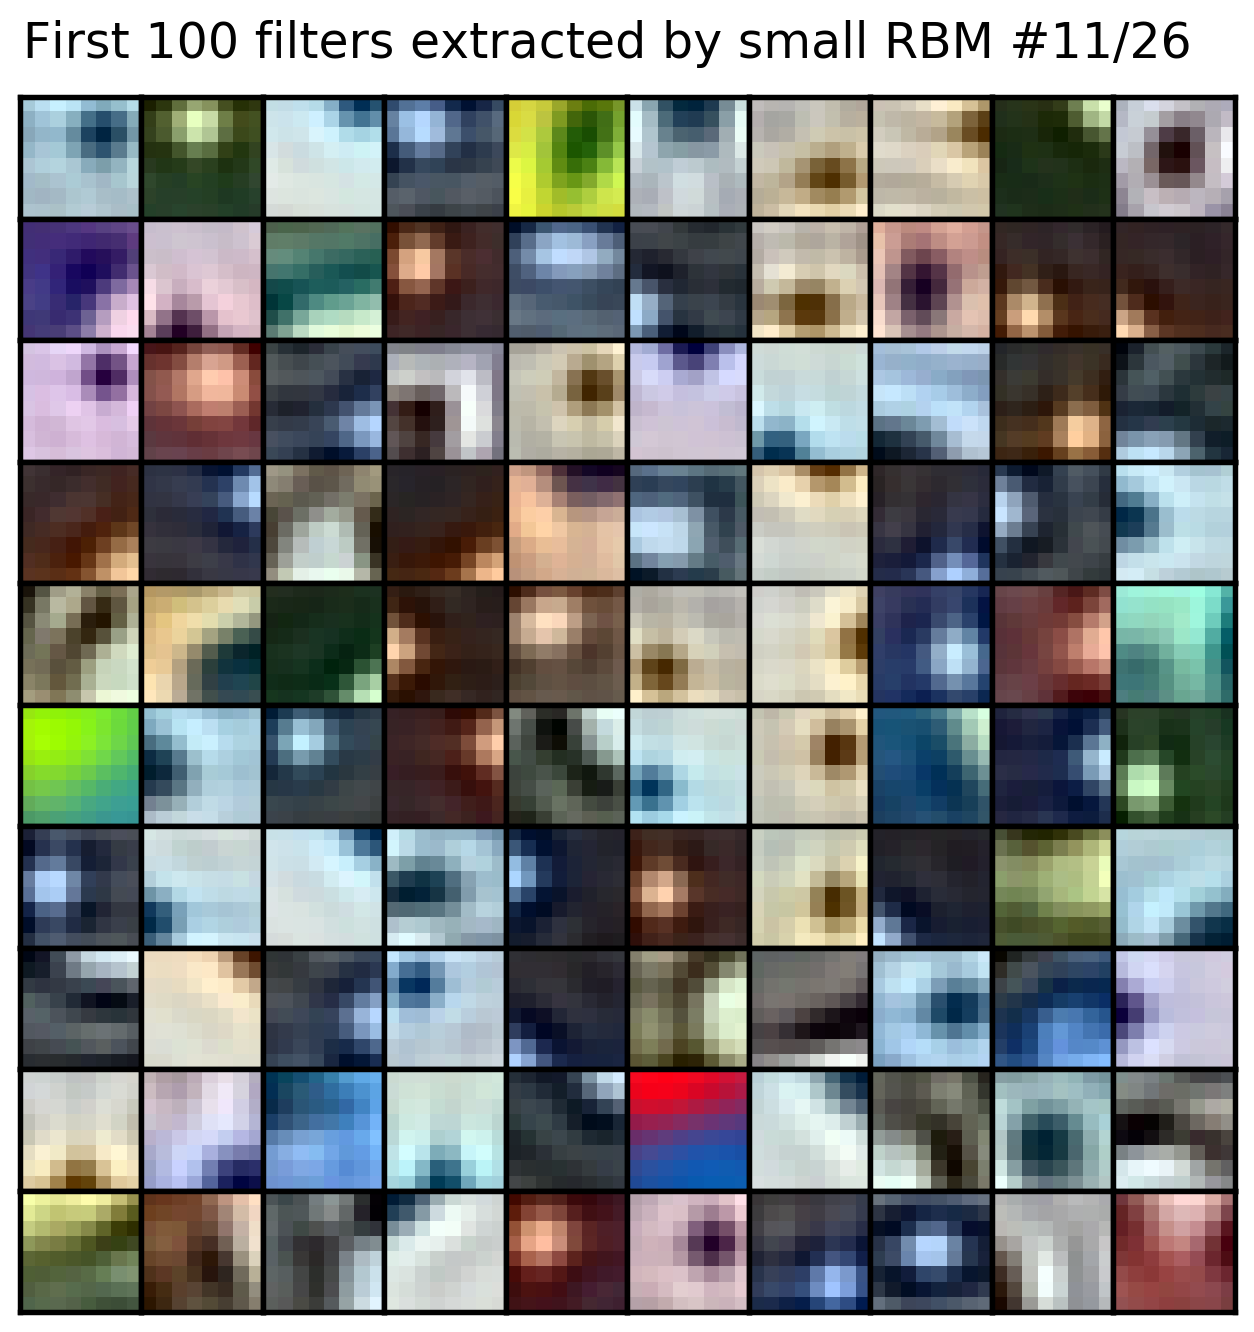
\includegraphics[width=1.6in]{dbm-cifar-latest/rbm_small_10.png}
\quad
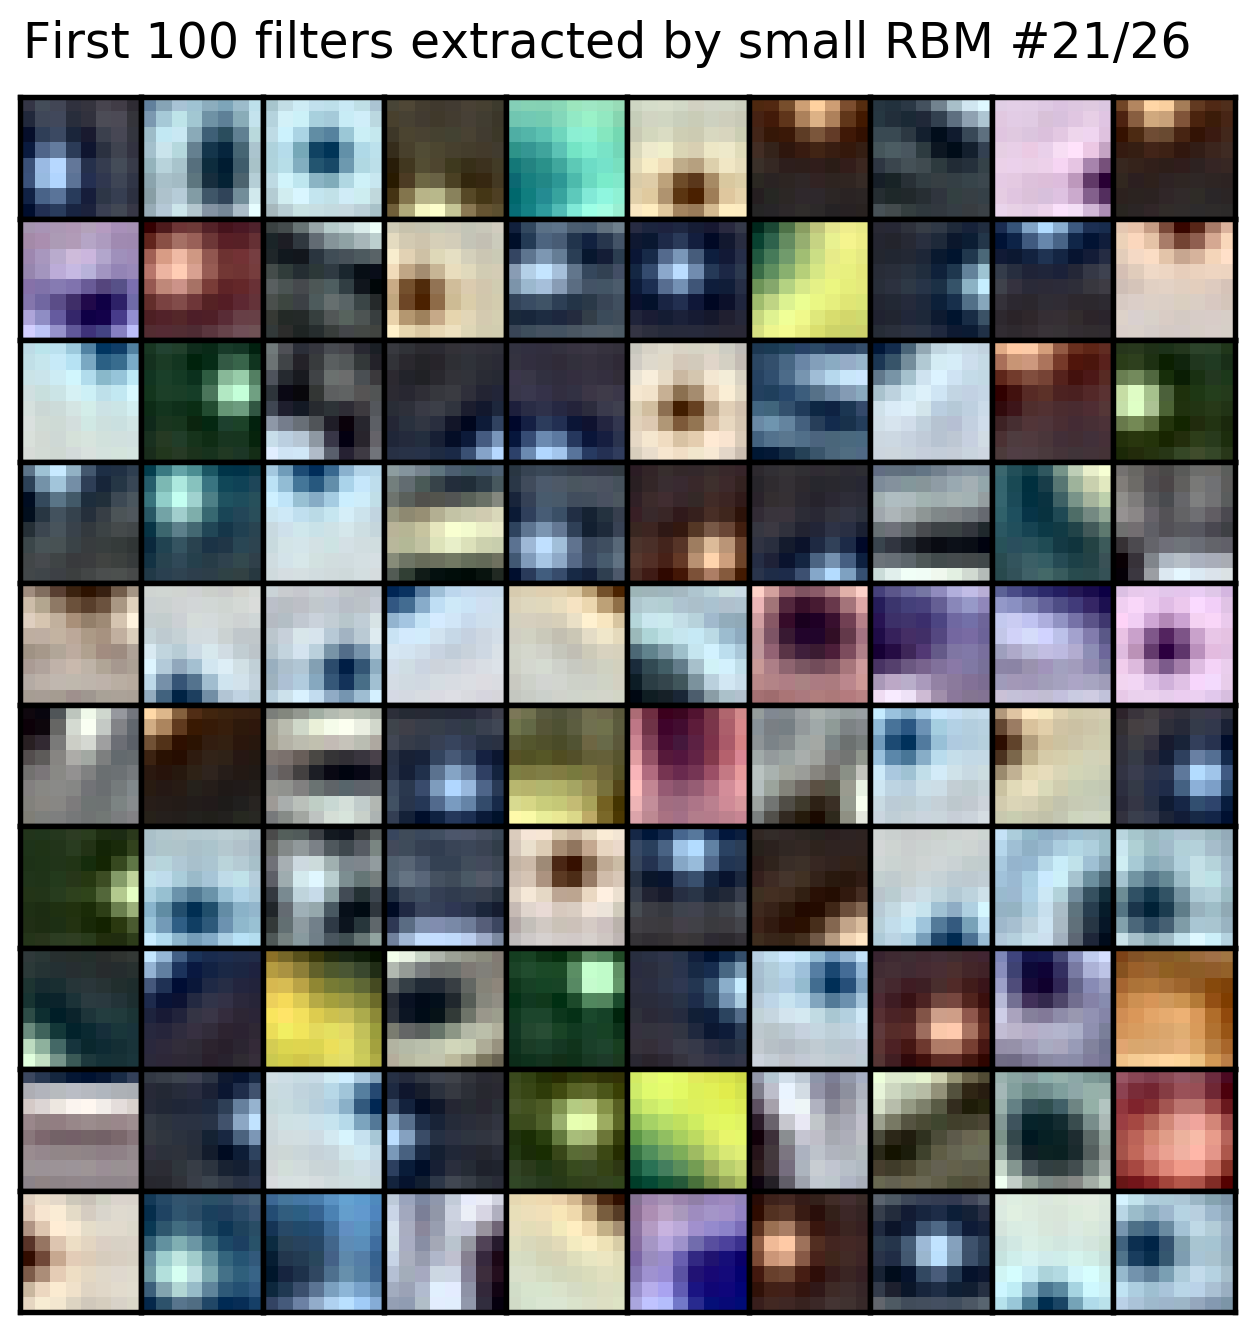
\includegraphics[width=1.6in]{dbm-cifar-latest/rbm_small_20.png}
\\[1em]
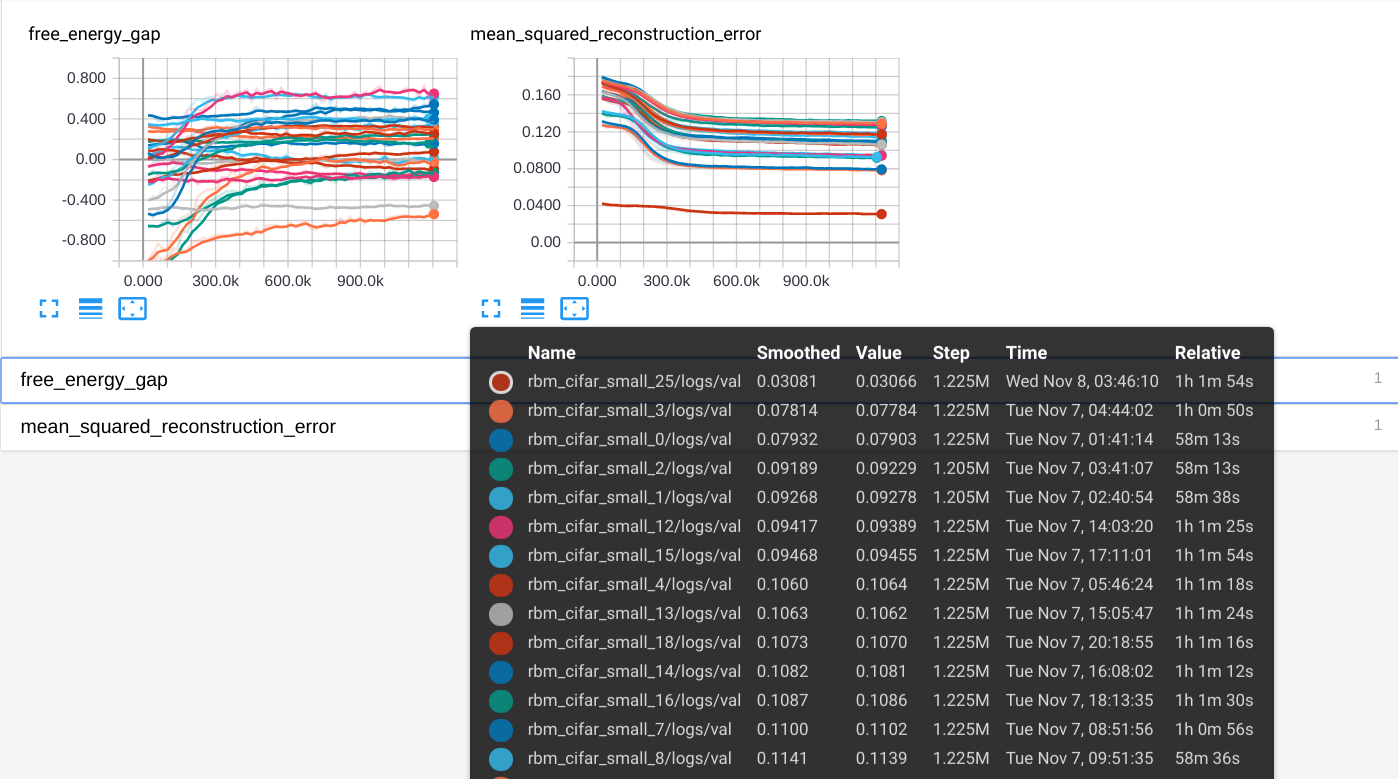
\includegraphics[width=6.4in]{dbm-cifar-latest/small_rbms.png}
\caption{\emph{Top}: Weight filters. \emph{Bottom}: reconstruction error and free energy gap of small RBMs. Notice different groups of RBMs based on their reconstruction errors. The lowest ($\approx$0.03) one has RBM which was trained on subsampled images. Next two ($\approx$0.078) were trained on top left and right corners of the images, which are the smoothest among all patches. Next 4 ($\approx$0.092) RBMs were trained on patches which are direct neighbors to top left and right, and after that come all the others.}.
\end{mdframed}
\end{figure}

\clearpage
\begin{figure}[h]
\begin{mdframed}
\centering
\includegraphics[width=2.2in]{dbm-cifar-latest/grbm.png}
\quad
\includegraphics[width=2.2in]{dbm-cifar-latest/mrbm.png}
\\[2em]
\includegraphics[width=2.2in]{dbm-cifar-latest/W1_joint.png}
\quad
\includegraphics[width=2.2in]{dbm-cifar-latest/W2_joint.png}
\\[2em]
\includegraphics[width=2.2in]{dbm-cifar-latest/cifar10.png}
\quad
\includegraphics[width=2.2in]{dbm-cifar-latest/samples.png}
\caption{\emph{Top}: Weight filters. \emph{Bottom}: random subset of training data and generated samples by DBM.}.
\end{mdframed}
\end{figure}

\clearpage
\begin{figure}[h]
\begin{mdframed}
\centering
\includegraphics[width=6.4in]{dbm-cifar-latest/grbm_metrics.png}
\\[6em]
\includegraphics[width=6in]{dbm-cifar-latest/dbm_msre.png}
\caption{\emph{Top}: reconstruction error and free energy gap of Gaussian RBM \emph{Bottom}: reconstruction error of DBM.}.
\end{mdframed}
\end{figure}
